% book example for classicthesis.sty
\documentclass[
  % Replace twoside with oneside if you are printing your thesis on a single side
  % of the paper, or for viewing on screen.
  oneside,
  twoside,
  12pt, letterpaper,
  footinclude=true,
  headinclude=true,
  cleardoublepage=empty
  spanish
]{scrbook}
%\usepackage[spanish]{babel}
\usepackage[linedheaders,parts,pdfspacing]{classicthesis}
\usepackage[utf8]{inputenc}%ñ y acentos
%\usepackage{mathptmx}% http://ctan.org/pkg/mathptmx   similar a times new roman
\usepackage{titletoc}
\usepackage{graphicx}
\usepackage{subfig}
\usepackage{tabularx}
\usepackage{listings}
\usepackage{float}%H figures place
\usepackage{longtable}
\usepackage{appendix}
\usepackage{datagidx}%para crear índices y glosarios
%\usepackage{showframe}  %Muestra los margenes de las paginas
%\usepackage{lipsum}
%\usepackage{amsmath}
%\usepackage{acronym}
%\usepackage{amsthm}
\usepackage{amssymb}
\usepackage[linesnumbered,vlined,ruled,algochapter,spanish]{algorithm2e}
%\usepackage[section]{placeins}
%\usepackage{titlesec}
%\usepackage{subcaption}
%\usepackage{xcolor}
\usepackage{color}
%\usepackage{easylist }
%\usepackage{enumerate}
%\usepackage{enumitem }
\usepackage{tocbibind}
\usepackage{letltxmacro}
\usepackage{epstopdf}    
\usepackage{gensymb}
\usepackage{stmaryrd}
\usepackage{siunitx}
\usepackage{placeins}
\usepackage{geometry}
\geometry{
	letterpaper,
	total={140mm,257mm},
	left=40mm,
	top=20mm,
	bottom=20mm,
	right=20mm,
	footskip=10mm,
}

% margenes
%\setlength{\textwidth}{140mm}
%\setlength{\oddsidemargin}{1mm}

%\areaset[current]{412pt}{761pt} % 686 (factor 2.2) + 33 head + 42 head \the\footskip

% este codigo da formato a los codigos
\lstset{
    frame=tb, % draw a frame at the top and bottom of the code block
    tabsize=4, % tab space width
    showstringspaces=false, % don't mark spaces in strings
    numbers=left, % display line numbers on the left
    commentstyle=\color{green}, % comment color
    keywordstyle=\color{blue}, % keyword color
    stringstyle=\color{red} % string color
}

\title{DESARROLLO DE UN SISTEMA QUE REPRESENTA OBJETOS
	CON GEOMETRÍAS SIMPLES USANDO ÁLGEBRA GEOMÉTRICA CONFORME}
\author{Villaseñor Altamirano Carlos Francisco}


\titlecontents{chapter}[1.5em]{}
{\contentslabel{2.3em}}
{\hspace*{-2.3em}}
{\titlerule*[1pc]{.}\contentspage}

\titlecontents{section}[2.3em]{}
{\contentslabel{2.3em}}
{\hspace*{-2.3em}}
{\titlerule*[1pc]{.}\contentspage}

\titlecontents{subsection}[3.8em]{} % note that 3.8 = 1.5 + 2.3
{\contentslabel{3.2em}}
{\hspace*{-3.2em}}
{\titlerule*[1pc]{.}\contentspage}

\titlecontents{figure}
[0em]{}
{\thecontentslabel\hspace*{1.5em}}
{}{\ \titlerule*[1pc]{.}\contentspage}

\titlecontents{table}
[0em]{}
{\thecontentslabel\hspace*{1.5em}}
{}{\ \titlerule*[1pc]{.}\contentspage}



\let\oldeqref\eqref
\RenewDocumentCommand\eqref{oom}{%
	\IfNoValueTF{#2}{\def\eqafter{}}{\def\eqafter{#2}}%
	\IfNoValueTF{#1}
	{\oldeqref{#3}}
	{(#1 \textup{\ref{#3}}\eqafter)}%
}



% se agrega el archivo del glosario

\newgidx{glosario}{Glosario}
\DTLgidxSetDefaultDB{glosario}
%centroide
%\newterm[description={}]{}
\newterm[description={Conexión funcional entre dos sistemas, programas, dispositivos o componentes de cualquier tipo},plural={interfaces}]{interfaz}
\newterm[description={Entorno de escenas u objetos de apariencia real, generado mediante tecnología informática}]{realidad virtual}
\newterm[description={Objeto complejo cuyos componentes se relacionan con al menos algún otro componente.}]{sistema}
\newterm[description={Hace referencia a las transformaciones conformes, en los cuales se mantienen los ángulos.}]{conforme}


\newterm[description={Del inglés "picture element" es la unidad básica de una imagen}, plural={pixeles}]{pixel}

\newterm[description={Es una figura geométrica que define una ubicación especifica del espacio.},plural={puntos}]{punto}

\newterm[description={Conjunto de puntos, habitualmente describen superficies. }, plural={nubes de puntos}]{nube de puntos}


\newterm[description={Elemento geométrico de dos dimensiones, que contiene infinitos puntos y rectas.},plural={planos}]{plano}
\newterm[description={elemento geométrico descrito por una superficie curva cuyos puntos equidistan al centro de esta.},plural={esferas}]{esfera}
\newterm[description={Elemento geométrico descrito por la revolución de un rectángulo.},plural={cilindros}]{cilindro}

\newterm[description={Representación visual de algún objeto}]{imagen}

%\newterm[description={}]{vector}

%\newterm[description={espacio vectorial}]{álgebra}

\newterm[description={Dispositivo eléctrico con la capacidad de manifestar magnitudes en variables eléctricas},plural={sensores}]{sensor}

\newterm[description={Subrutina perteneciente a la clase de algún programa para realizar una acción}, ]{método}

\newterm[description={Conjunto de instrucciones ordenadas y finitas para realizar alguna actividad}]{algoritmo}
\newterm[description={Programa que permite al sistema operativo interaccionar con un periférico}]{controlador} 
\newterm[description={Programa que remueve parte de la información dada. }]{filtro} 


%ToF
%AG
%agc
%ae
%RANSAC
%PCL




\renewcommand\tablename{Tabla}
\renewcommand\figurename{Figura}



\begin{document}
    % portada y todo lo que va antes del índice
    \frontmatter
    \begin{titlepage}
%\begin{addmargin}[-1cm]{-3cm}
\centering
\vfill
        \centering
        \begin{tabular}{lll}
        	
        	\begin{minipage}[c][40mm][l]{0.15\textwidth}
            {\includegraphics[height = 35mm]{00FrontBackMatter/imagenes/ipn.jpg}}
        \end{minipage}
             &  
             \begin{minipage}[c][40mm][c]{0.59\textwidth}
                \centering
                {\scshape\large\bfseries INSTITUTO POLITÉCNICO NACIONAL}\\
                \vspace{0.5cm}
                {\scshape  CENTRO DE INNOVACIÓN Y DESARROLLO TECNOLÓGICO EN CÓMPUTO\par}
            \end{minipage}
             &
             \begin{minipage}[c][40mm][l]{0.2\textwidth}
            \includegraphics[height = 3.1cm]{00FrontBackMatter/imagenes/cidetec.png}\\
        \end{minipage}
             \\
        \end{tabular}
      \\
	\vspace{2.5cm}
	{ \large \bfseries DESARROLLO DE UN SISTEMA QUE REPRESENTA OBJETOS
	CON GEOMETRÍAS SIMPLES USANDO ÁLGEBRA GEOMÉTRICA CONFORME\par}
	\vspace{1.5cm}
	{ \large \bfseries T E S I S\par}
	\vspace{1.5cm}
	{ \large Que para obtener el grado de:\par}
	{ \large \bfseries Maestriá en Tecnología de Cómputo\par}
	\vspace{2cm}
	{ \large  Presenta:\par}
	{ \large \bfseries \textsc{ Carlos Francisco Villaseñor Altamirano}\par}
	\vspace{2cm}
	{\large Directores de la tesis:\par}
	{\large \bfseries \textsc{M. en C. Marco Antonio Valencia Reyes}}\\
	{\large \bfseries \textsc{Dr. Gabriel Sepúlveda Cervantes}}
	\vfill

    % Bottom of the page
	{Ciudad de México \hfill Noviembre de 2018\par}
%\end{addmargin}
\end{titlepage}







%
    
    %\begin{addmargin}[-1cm]{-3cm}
        %	\includegraphics[width=1.5\textwidth]{FrontBackMatter/Captura2.JPG}
        %	\includegraphics[width=1.5\textwidth]{FrontBackMatter/Captura1.JPG}
    %\end{addmargin}
    
    %\clearpage
    %%*******************************************************
% Declaration
%*******************************************************
\pdfbookmark[0]{Declaration}{declaration}
\chapter*{Advertencia}
\thispagestyle{empty}

“Este documento contiene información desarrollada por la Escuela
Superior de Cómputo del Instituto Politécnico Nacional, a partir de datos y
documentos con derecho de propiedad y por lo tanto, su uso quedará
restringido a las aplicaciones que explícitamente se convengan.”\\
\\
La aplicación no convenida exime a la escuela su responsabilidad técnica y
da lugar a las consecuencias legales que para tal efecto se determinen.\\
\\
Información adicional sobre este reporte técnico podrá obtenerse en:\\
 \\
La Subdirección Académica de la Escuela Superior de Cómputo del Instituto
Politécnico Nacional, situada en Av. Juan de Dios Bátiz s/n Teléfono:
57296000, extensión 52000. 

    
\chapter{Resumen}
En este trabajo se presenta una propuesta para el desarrollo de una interfaz que permita la interacción de objetos reales con un mundo virtual, usando un clasificador objetos son representados por geometrías simples. Modificando el proceso de clasificación usando álgebra geométrica conforme (AGC) se plantea mejorar el proceso.


Con el sensor Kinect se obtienen las nubes de puntos de los objetos, se realiza la estimación de parámetros para los modelos de la esfera, el plano y el cilindro, usando el método RANSAC, y posteriormente seleccionar el modelo que mejor represente al objeto.

El sistema se compara contra el mismo pero en lugar de usar AGC utiliza métodos RANSAC de la biblioteca Point Cloud Library (PCL). Los resultados muestran valores similares entre los sistemas así como algunas ventajas individuales para cada sistema.
 

\chapter{Abstract}
It is presented the development of an interface between real objects and virtual reality, with the help of an object classifier the objects are represented by simple geometric forms.  By modifying the method using conformal geometric algebra (CGA) is expected to improve the classifier.

A parameter estimation is made for the sphere, plane, and cylinder using the RANSAC estimator and the Kinect to get the point clouds.

The system is compared with a modified version of itself which use the RANSAC methods from the Point Cloud Library (PCL) instead of the CGS methods, the results show some similarity between systems and some benefits for each system.


    %%*******************************************************
% Dedication
%*******************************************************
%\thispagestyle{empty}
\pdfbookmark[1]{Dedication}{Dedication}
\chapter{Dedicatoria}
\vspace*{3cm}

\begin{center}
to someone special
\end{center}

    %%*******************************************************
% Acknowledgments
%*******************************************************
\pdfbookmark[1]{Acknowledgements}{acknowledgements}
\chapter*{Agradecimientos}
 Primero, me gustaría agradecer sinceramente a mis directores de tesis Mtr. Marco Antonio Dorantes Gonzáles y Dr. Gabriel Sepúlveda Cervantes por su esfuerzo y dedicación.
\\
 Al profesor Mtr. Marco Antonio Dorantes y a su esposa Mtr. Martha Rosa  Cordero por ser los que me permitieron expandir mis ideas y conocimientos así como enseñarme a disfrutar del trabajo. 
 \\
 Y al  Dr. Gabriel Sepúlveda Cervantes y a todo el equipo de EDISSA por el gran apoyo que me brindaron para poder elegir el camino que quiero seguir.
 \\
También quiero dedicar este trabajo a mis padres, Juan Carlos Villaseñor Rios y Silvia Beatriz Altamirano Morales, que gracias a ellos hoy estoy aquí, y que sin su amor, cariño, esfuerzo o dedicación nada de esto hubiera sido posible, también quiero agradecer a mis hermanas Ana Beatriz y Silvia Leticia que me apoyaron y ayudaron en todo momento, al igual que toda mi familia. 
\\
Sin olvidar agradecer a todos los profesores que me enseñaron a como superar obstáculos en la vida y con especial cariño al Lic. Juan Vera Romero un gran profesor dentro y fuera del aula y un gran amigo, así también debo agradecer el tiempo y ayuda de una muy querida amiga la ingeniera Aura Jesid que me estuvo ayudando durante todo el desarrolló del proyecto.
\\
Por ultimo quisiera agradecer a todos y cada uno de mis amigos que me acompañaron en esta etapa de mi vida, ya que llegue a pasar mas tiempo con ellos que con mi propia familia, convirtiéndose así en la familia que yo elegí.
    %*******************************************************
% Table of Contents
%*******************************************************
%\pdfbookmark[1]{\contentsname}{Contenido}
\setcounter{tocdepth}{1} % <-- 2 includes up to subsections in the ToC
\renewcommand{\thesection}{\arabic{chapter}.\arabic{section}}


\renewcommand{\thefigure}{\arabic{chapter}.\arabic{figure}}
\renewcommand{\thetable}{\arabic{chapter}.\arabic{table}}

\renewcommand{\bibname}{Referencias} %%no name

\renewcommand{\contentsname}{Contenido}
\tableofcontents 

%*******************************************************
% List of Figures and of the Tables
%*******************************************************

%*******************************************************
% List of Figures
%*******************************************************   
\pdfbookmark[1]{\listfigurename}{lof}

\renewcommand{\listfigurename}{Índice de Figuras}
\listoffigures

%*******************************************************
% List of Tables
%*******************************************************
\pdfbookmark[1]{\listtablename}{lot}
\renewcommand{\listtablename}{Índice de Tablas}
\listoftables
  
%*******************************************************
% List of Listings
%******************************************************* 
\pdfbookmark[1]{lstlistingname}{loc}
\renewcommand{\lstlistlistingname}{Índice de Códigos}
\renewcommand*{\lstlistingname}{Código}
\lstlistoflistings 
   
   \newcommand{\listofalgorithmes}{\tocfile{\listalgorithmcfname}{loa}}
   \listofalgorithmes
%----------------------------------------------------------------------------------------
%	ABBREVIATIONS
%----------------------------------------------------------------------------------------

\printterms[columns=1,style=align]

    
    % inicio del documento
    \mainmatter
    
    \chapter{Introducción}
        %\section{Motivación}
Actualmente los sistemas de \gls{realidad virtual} se encuentran en auge tanto en el ámbito comercial como en el desarrollo tecnológico, esto gracias al incremento en la capacidad de cómputo y la reducción del tamaño de algunos dispositivos electrónicos. Tecnologías como Google Cardboard, HTV VR Headset, Microsoft HoloLens, etc. han sido tecnologías pioneras permitiendo al usuario experimentar la realidad virtual de forma más personal e intuitiva.\\

De manera similar a cuando la tecnología de las pantallas táctiles llegó a los celulares y forzaron la creación de nuevas interfaces para la interacción entre el usuario y la computadora, las nuevas tecnologías de realidad virtual se enfrentan al desarrollo de nuevas \glspl{interfaz}.\\

Estas nuevas interfaces son particularmente complicadas ya que se busca una interacción natural e intuitiva para el usuario, y que no solo se busca la interacción entre usuario y el mundo virtual, algunas empresas como Mircosoft con el proyecto de HoloLens apuntan a la intersección entre la realidad virtual y la realidad aumentada (realidad mixta), esto conlleva una interacción entre elementos reales, elementos virtuales y el usuario o usuarios.\\

El problema con la interacción entre el usuario y el mundo virtual se ha tratado usando sistemas de captura de movimiento como los de la empresa VICON \cite{vicon}, que usando cámaras infrarrojas son capaces de obtener la pocición de un objeto que cuenta con reflectores de luz infrarroja. El problema es que estos sistemas son delicados y costosos, otra propuesta es presentada por Microsoft en los HoloLens y el Kinect que usan un sitema de mapeo del entorno usando luz infraroja y la tecnologia ToF (del ingles Time of figth) la cual calcula la distancia entre el dispocitivo y el entorno usando el tiempo que tarda la luz en rebotar en un objeto, como desventaja este metodo no disingue entre difeentes objetos. Esto deja un area de desarrollo para nuevas interfaces.\\
%el cual puede ser desglosado en investigaciones más simples.\\




        \section{Marco teórico}

Para el desarrollo de este trabajo se abordan temas como la obtención de datos (visión por computadora), clasificación (RANSAC) y la implementación de AGC.  Por lo cual, a continuación, se describen los conceptos necesarios para el desarrollo.

\subsection{Representación Digital}

Una imagen digital es guardada según el formato de imagen (TIFF, BMP, JPEG, etc.), pero todas las imágenes luego de su interpretación son representadas en una computadora por un arreglo bidimensional de \glspl{pixel}.\\

El arreglo de píxeles se puede ver como un conjunto de matrices numéricas, dependiendo la representación del píxel (RGB, CMY, RGBA, CMYA, etc.) son los canales necesarios para representarlo por completo. Así una imagen en RGB (rojo, verde, azul por sus siglas en inglés) cuenta con tres canales, cada canal define la intensidad de cada color, así para mostrar una imagen $MxN$ en RGB es necesario tres matrices de $M$ filas y $N$ columnas.\\

De esta manera es posible generar una imagen nueva a partir de otras realizando operaciones sobre imágenes como la suma, resta y multiplicación, aplicando una transformación como se muestra en la ecuación \eqref[ec.]{eq:transfimg}.\\

\begin{equation}
\label{eq:transfimg}
q(x,y)=f(p_1(x,y),p_2(x,y))
\end{equation}
Donde $p_1$ es un píxel de la imagen 1 y $p_2$ un píxel de la imagen 2 y $q(x,y)$ el píxel resultante de la nueva imagen \cite{martinsanz2007ejercicios}.\\

Una \gls{nube de puntos} se describe como el conjunto de puntos en un espacio dado o una estructura de datos usada para representar una colección de puntos \cite{weinmann2016reconstruction}. Al trabajar con nubes de puntos se pueden pensar en ellas como una imagen de tres dimensiones y en lugar de un píxel se trabajan sobre \glspl{punto}. Al igual que las imágenes.\\

A diferencia de una \gls{imagen} una nube de puntos puede o no estar organizada en filas y columnas, sensores como el Kinect en los que se obtiene una imagen de profundidad se obtiene una nube de puntos de $MxN$ puntos, mientras que otras nubes de puntos tienden a ser solo una lista $Mx1$ de puntos en el espacio \cite{Rusu_ICRA2011_PCL}.\\


\subsection{Sensor Kinect}

En el desarrollo de vídeo juegos, la competencia entre grandes empresas ha dado como resultado en una variedad de dispositivos que le permiten al usuario una interacción más natural con entornos virtuales. Estos dispositivos son variados tanto en sus componentes físicos como en la forma de interacción. unos de los dispositivos más conocidos son el Wii Mote, PS/Move y el Kinect.\\

Para la consola Wii de Nintendo se usa un Wii Mote, mostrado en la figura \ref{fig:WiiMote}, que, con el uso de una barra de leds infrarrojos y sensores de posición y aceleración, es capaz de obtener su posición respecto la barra de leds \cite{UsodelKi56:online}.\\
\begin{figure}[!htb]
	\centering
	\includegraphics[width=0.4\textwidth]{01Introduccion/imagenes/wiiMote.JPG}
	\caption{Control Wii Mote de Nintendo} 
	\label{fig:WiiMote}
\end{figure}


En el caso del PlayStation de Sony, que usa un PS/Move, mostrado en la figura \ref{fig:psMove}, se usa una cámara de vídeo que, junto con sensores de posición y aceleración, se realiza esta interacción.\\

\begin{figure}[!htb]
	\centering
	\includegraphics[width=0.2\textwidth]{01Introduccion/imagenes/PsMOve.JPG}
	\caption{Control PS/Move de Sony} 
	\label{fig:psMove}
\end{figure}

Mientras que Xbox de Microsoft optó por un dispositivo realizado por la empresa PrimeSense llamado Kinect, el cual integra micrófonos, un motor, un emisor infrarrojo, una cámara de vídeo a color y otra infrarroja \cite{UsodelKi56:online}, el dispositivo se muestra en la figura \ref{fig:kinect1} \cite{Microsof29:online}. Usando la cámara infrarroja el Kinect detecta la profundidad de objetos usando una técnica llamada tiempo de vuelo (Time of Flight ToF), en la cual se obtiene el tiempo que tarda un rayo de luz en rebotar en un objeto, sabiendo la velocidad del rayo de luz y el tiempo desde su emisión hasta que es captado por la cámara, se calcula la distancia del objeto al sensor\cite{Lachat2015}.\\

\begin{figure}[!htb]
	\centering
	\includegraphics[width=0.7\textwidth]{01Introduccion/imagenes/xbox360kinect.JPG}
	\caption{Sensor Kinect 1} 
	\label{fig:kinect1}
\end{figure}

El dispositivo Kinect cuenta con dos versiones el primero se anunció con la consola Xbox 360 en el 2010 y el Kinect 2.0, mostrado en la figura \ref{fig:kinect}, se anunció junto a la Xbox One en 2013 los cuales cuentan con las características mostradas en la tabla \ref{tab:Kinect} \cite{UsodelKi56:online}.\\

% Please add the following required packages to your document preamble:
% \usepackage{graphicx}
\begin{table}[!htb]
	\centering
	\caption{Tabla comparativa de los modelos del Kinect}
	\label{tab:Kinect}
	\begin{tabular}{lll}
		\hline
		Característica                    & Kinect 1          & Kinect 2            \\ \hline
		Cámara de color                   & 640 x 480 @30 fps & 1920 x 1080 @30 fps \\
		Cámara de profundidad             & 320 x 240         & 512 x 424           \\
		Profundidad Máxima                & $\sim$4.5 m       & $\sim$4.5 m         \\
		Distancia de profundidad mínima   & 40 cm             & 50 cm               \\
		Visión de campo horizontal        & 57 grados         & 70 grados           \\
		Visión de campo vertical          & 43 grados         & 60 grados           \\
		Motor de inclinación              & si                & no                  \\
		Uniones definidas para esqueletos & 20 uniones        & 26 uniones          \\
		Esqueletos rastreados             & 2                 & 6                   \\
		Estándar USB                      & 2.0               & 3.0                 \\ \hline
	\end{tabular}%
\end{table}

\begin{figure}[!htb]
	\centering
	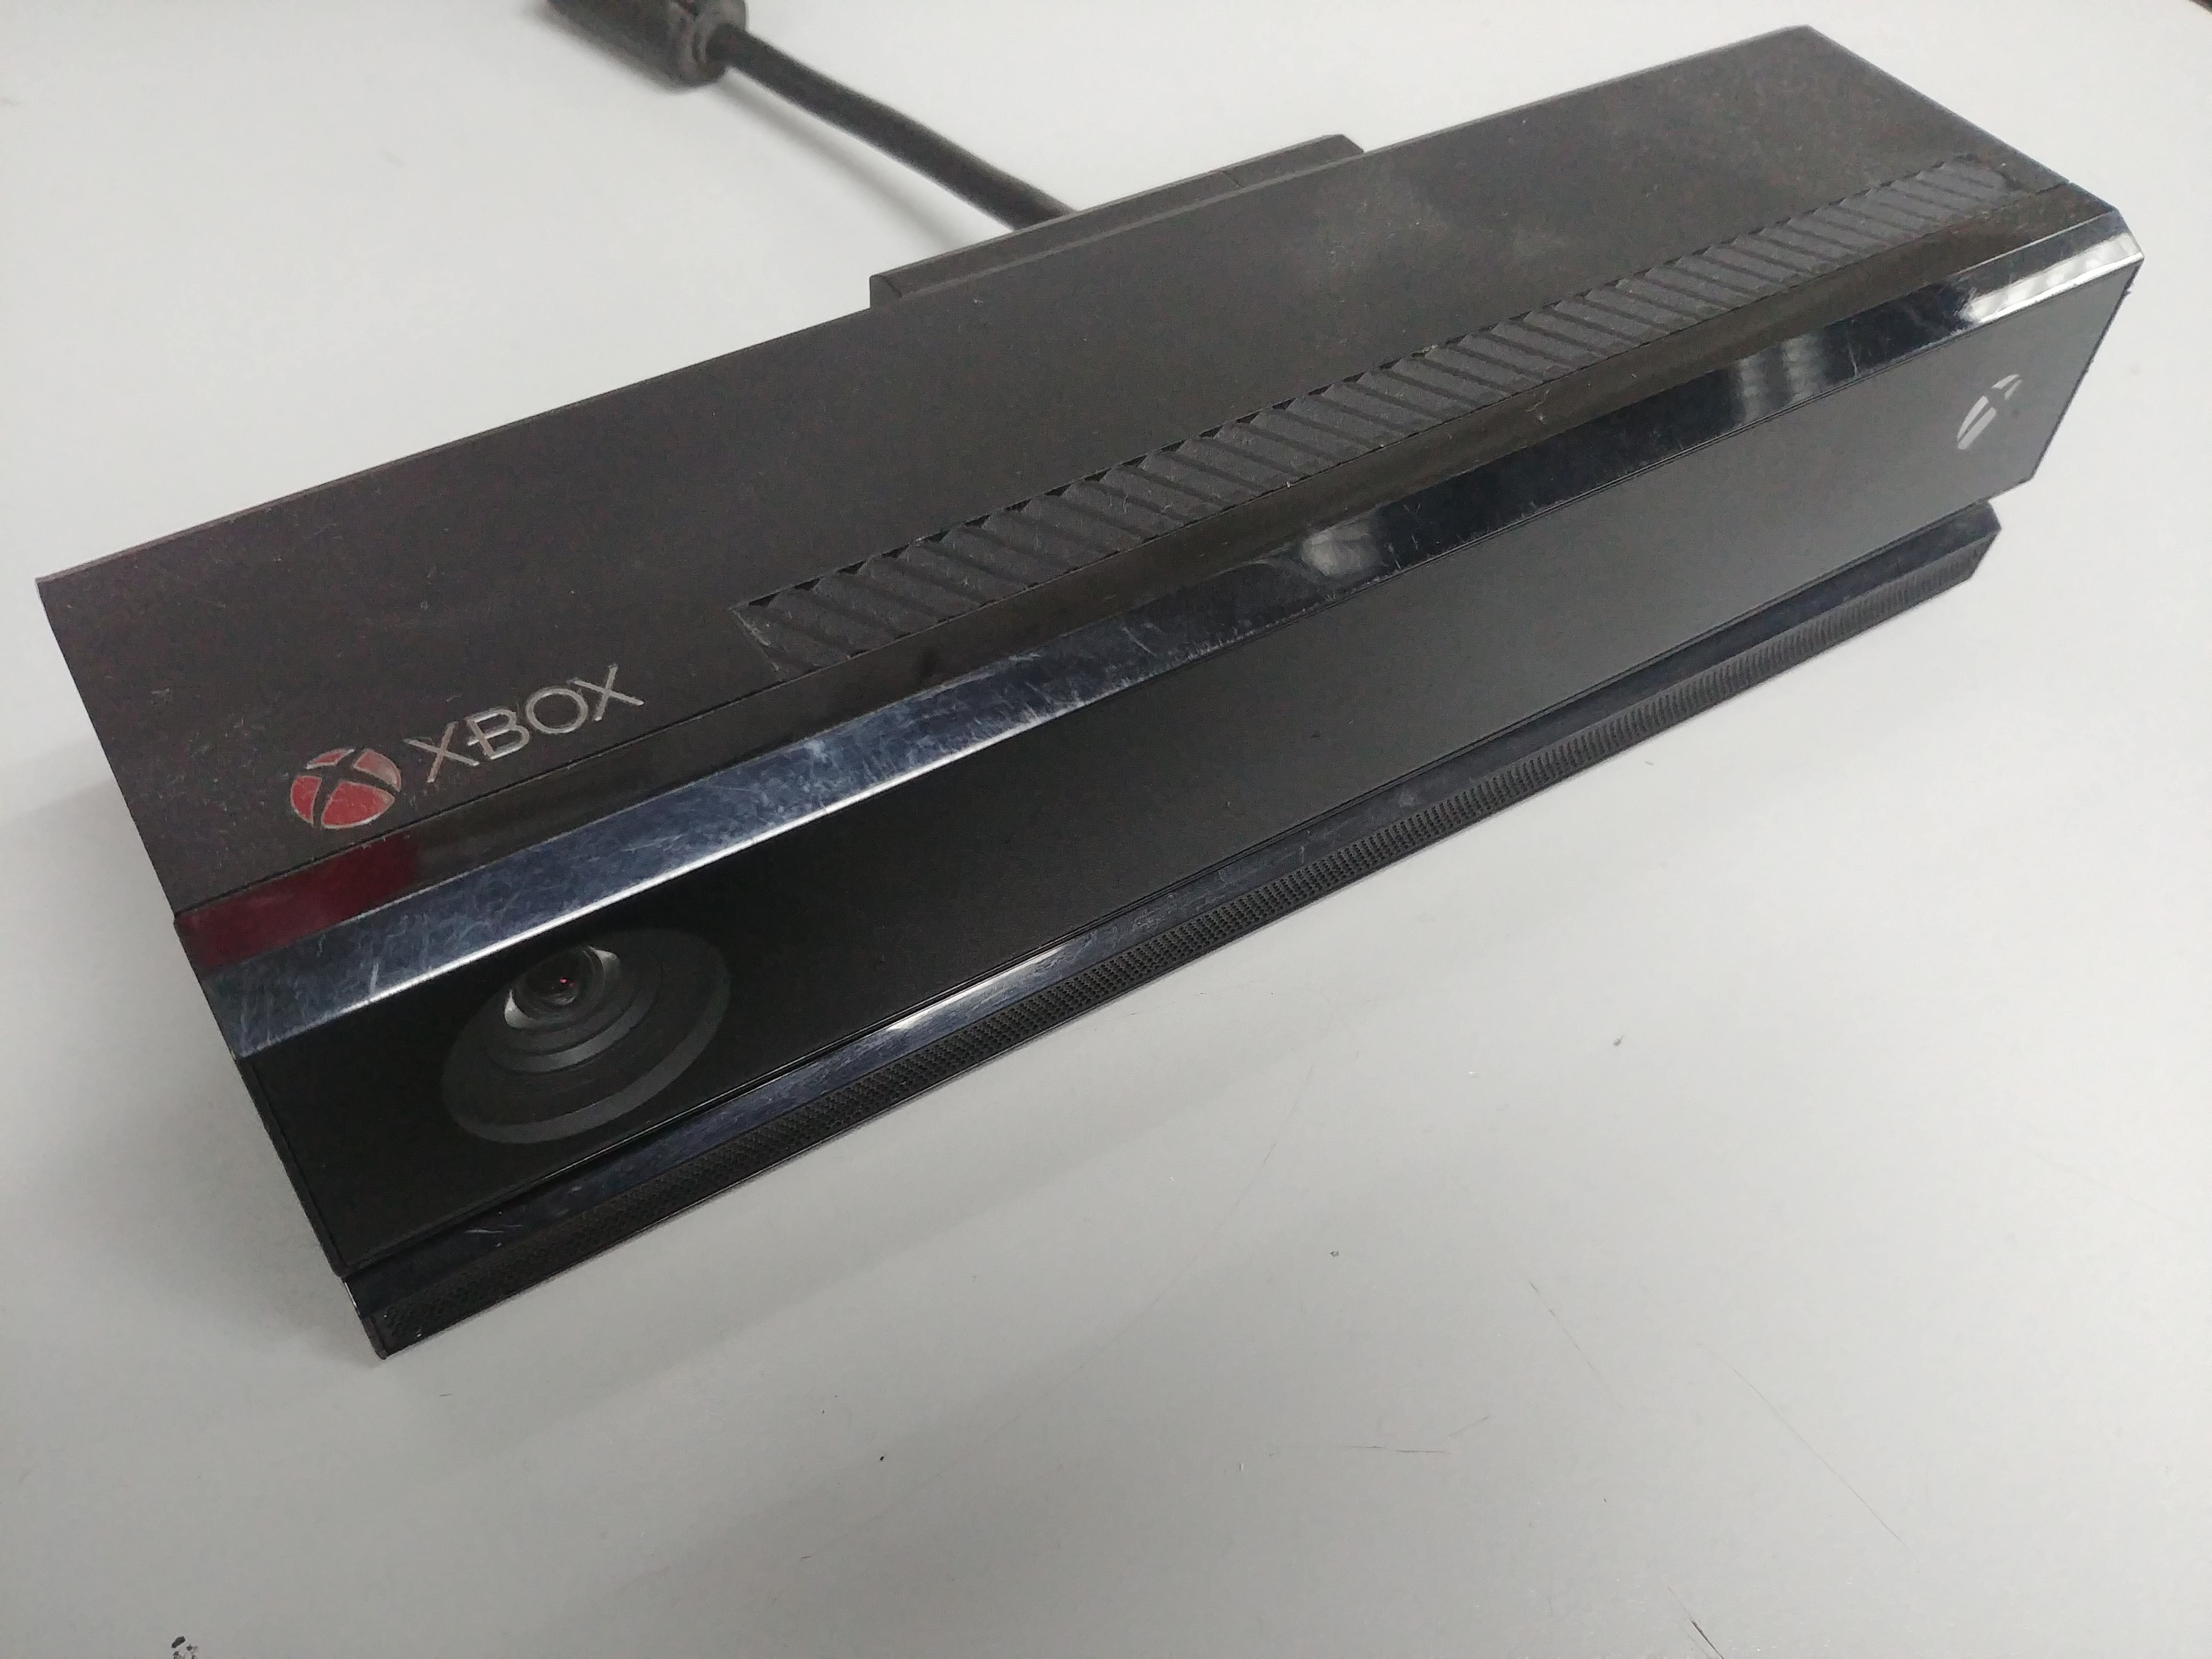
\includegraphics[width=0.6\textwidth]{02Desarrollo/Preprocesamiento/imagenes/20181017_182538[1].jpg}
	\caption{Sensor Kinect 2.0} 
	\label{fig:kinect}
\end{figure}



\subsection{Visión Por Computadora}

La visión por computadora trata de describir el mundo que vemos a partir de una o varias imágenes y reconstruir sus propiedades, como forma, color e intensidad de luz, tratando de imitar la visión de una persona. Es usada en gran cantidad de aplicaciones como: reconocimiento óptico de letras, inspección de productos en fábricas, modelado 3D, reconocimiento facial, etc. \cite{CompVisionSpringer}.\\

Se llevan a cabo varios procesos antes de someter una imagen a reconocimiento, esto sirve para resaltar puntos importantes, facilitar la detección de características, eliminar ruido, etc. Estos procesos son diferentes según el problema a tratar, pero ayudan en gran medida mejorar el reconocimiento de objetos por la computadora, y en conjunto se les conoce como preprocesamiento de imagen.\\

Para que la computadora sea capaz de reconocer su entorno existen diferentes técnicas como la selección de puntos característicos o de marcadores en un objeto visto por dos o más cámaras y el cálculo de su posición usando las imágenes obtenidas; también el análisis de la perspectiva de una imagen (buscando rectas o círculos) o algoritmos de búsqueda como los usados en sistemas con inteligencia artificial (redes neuronales o K vecinos más próximos). \\

\subsubsection{Transformada de Hough}

El algoritmo usado para la transformada de Hough (TH) fue patentado en 1962 por P. Hough como un método para reconocer líneas rectas y más tarde se extendió para detectar figuras complejas, como círculos, polígonos o elipses, y se le llamó la transformada de Hough generalizada, esta técnica permite la detección de los parámetros de un modelo usando un sistema de votación en el cual cada dato favorece al conjunto de parámetros que satisfacen al modelo para dicho dato,  aunque la TH se ha visto que tiene dificultad para trabajar con modelos con gran cantidad de incógnitas\cite{CompVisionKinecthough}. \\

Por ejemplo, si quisiéramos detectar una línea recta, lo primero que se necesita es saber la definición de una línea recta, esta está definida como la sucesión de puntos que se extienden en una misma dirección. y su representación matemática está dada por la ecuación \eqref[ec.]{eq:linea}\\

\begin{equation}
\label{eq:linea}
y=mx+b
\end{equation}

Donde $x$ y $y$ son las variables, $m$ la pendiente de la línea y $b$ la intersección de la línea sobre el eje $y$ respecto del origen. En este ejemplo $m$ y $b$ son los parámetros de una línea recta, los cuales describen la línea que está buscando.\\

Luego de conocer el modelo de la línea que se está buscando se necesitan los posibles candidatos, es decir de una imagen cuales son los posibles puntos que pertenecen a una línea, una forma de obtenerlos es el resaltar los bordes de una imagen, recordando que un borde se entiende como un cambio súbito de un valor, para esto se pueden realizar varios filtros, como el filtro de Sobel, Roberts, Prewitt, etc. , de los cuales se obtiene una imagen binaria, con un valor de uno indicando la presencia de un borde y cero en el caso contrario. \\

Ya obtenidos los posibles puntos, lo siguiente es aplicar la TH a cada punto, lo que realiza la TH es describir el modelos usando los parámetros, en lugar de tener los ejes $(x,y)$ se usan los ejes $(m,b)$, de esta forma un punto en $(x,y)$ representa una línea en el espacio de parámetros $(m,b)$, y una línea en $(x,y)$ se representa como un punto. Estas consideraciones son importantes ya que encontrando la intersección de líneas en el espacio de parámetros $(m,b)$ se consigue una línea en $(x,y)$, ya que  no se conoce la intersección de estas líneas pueden estar en el infinito, se utilizan las coordenadas polares de esta manera las líneas se forman por funciones periódicas y le es más fácil encontrar estas intersecciones a la computadora, la representación de la línea en coordenadas polares queda descrita como en la ecuación \eqref[ec.]{eq:polar}, donde $p$ es la distancia que e existe del origen al punto $(x,y)$, y $\theta$ es el ángulo del vector perpendicular a la recata y que pasa por el origen.  \\
\begin{equation}
\label{eq:polar}
y=(-\frac{cos\theta}{sin\theta})*x+(\frac{p}{sin\theta})
\end{equation}           
Escribiendo la ecuación en función de $\theta$  y despejando $p$ se obtiene la ecuación \eqref[ec.]{eq:polarLine}, que para cada punto $(x,y)$ se obtiene una sinusoide en el espacio de parámetros $(p,\theta)$ donde $\theta \in [0,\pi)$ y $p \in \mathbb{ R}$ o $\theta \in [0,2\pi)$ y $p \geq 0$, de esta manera un punto vota por toda una familia de rectas, cada que una sinusoide interseca con otra votan por la recta que corresponde al punto $p,\theta)$, y los más votados son los que más probabilidad tienen de ser una de las líneas que se buscan.          

\begin{equation}
\label{eq:polarLine}
p=x*cos\theta +y*sin\theta
\end{equation}  

\subsection{RANSAC}

Del inglés RANdom SAmple Consensus (RANSAC) es un \gls{metodo} iterativo para estimar parámetros de algún modelo matemático, es decir, encuentra el conjunto de parámetros para un modelo matemático que mejor describe a un conjunto de datos \cite{Fischler1981}. \\

Este método es no determinista ya que realiza el muestreo de forma aleatoria y dependiendo de la distribución de los datos es la precisión que se puede obtener. Entre más repeticiones se realicen mayor precisión se tendrá ya que se habrán usado un mayor número de combinaciones.\\

En la figura \ref{fig:RANSAC} se muestra el diagrama de flujo que se sigue para implementar el \gls{algoritmo} RANSAC.\\

\begin{figure}[!htb]
	\centering
	\includegraphics[width=1\textwidth]{01Introduccion/imagenes/RANSAC.jpeg}
	\caption{Diagrama de flujo del método RANSAC}
	\label{fig:RANSAC}
\end{figure}

\subsection{Álgebra Geométrica (AG)}

En matemáticas es común el uso de álgebras de Clifford y Grassmann, aunque por cuestiones prácticas para la ingeniería se prefiere trabajar con el álgebra vectorial para espacios euclidianos (AE) propuesta por Josiah Willard Gibbs en el siglo XIX, la cual se enfoca a la manipulación de tres dimensiones y los números escalares,  aunque últimamente el uso de AG ha sido necesario por la demanda de los físicos para trabajar en más dimensiones \cite{FoundOfAGC}.\\

Al hablar de álgebras nos referimos a un con junto de operaciones con estructura algebraica. Para tener una estructura algebraica de deben cumplir las siguientes reglas. Dado el conjunto $A(S)$ de todas las aplicaciones inyectivas de $S$ sobre sí mismo, siendo $A(s)$ un conjunto no vacío \cite{herstein1988algebra}:

\begin{enumerate}
	\item Cerradura, a saber, si $f$, $g \in A(S)$, entonces $fg \in A(S)$. Se dice que $A(S)$ es cerrado respecto a este producto.
	\item Asociatividad, esto es, dadas $f$, $g$, $h \in A(S)$, entonces $f(gh) = (fg)h$.
	\item Existencia de un elemento unidad, a saber, existe un elemento	particular $i \in A(S)$ (la aplicación identidad) tal que $fi = if = f$ para toda $f \in A (S)$.
	\item Existencia de inversas, esto es, dada $f \in A(S)$ existe un elemento en $A(S)$, denotado por $f^{-1}$, tal que $ff^{-1} = f^{-1}f = i$. 
\end{enumerate}


El álgebra vectorial $V$ está definido por el espacio vectorial conformado por el conjunto de objetos denominados vectores, junto con dos operaciones binarias llamadas suma y multiplicación por un escalar que satisface los axiomas \cite{grossman2008algebra}:

\begin{enumerate}
	\item Si $x \in V$ y $y \in V$, entonces $x+y \in V$ (cerradura bajo suma)
	\item Para todo $x$,$y$,$z \in V$, $(x+y)+z=x+(y+z)$ (ley asociativa de la suma de vectores)
	\item Existe un vector $0 \in V$ tal que para todo $x \in V$, $x+0=0+x=x$ (el $0$ se llama vector cero o idéntico aditivo)
	\item Si $x \in V$, existe un vector $-x \in V$ tal que $x+(-x)=0$ ($-x$ se llama inverso aditivo de $x$)
	\item Si $x$ y $y \in V$, entonces $x+y=y+x$ (ley conmutativa de suma de vectores)
	\item Si $x \in V$ y $\alpha$ es un escalar, entonces $\alpha x \in V$ (cerradura bajo multiplicación por un escalar)
	\item Si $x$ y $y \in V$ y $\alpha$ es un escalar, entonces $\alpha(x+y) =\alpha x+ \alpha y$ (primera ley distributiva)
	\item Si $x \in V$ y $\alpha$ y $\beta$ son escalares, entonces $(\alpha+\beta)x= \alpha x+ \beta x$ (segunda ley distributiva)
	\item Si $x \in V$ y $\alpha$ y $\beta$ son escalares, entonces $\alpha(\beta x)=(\alpha \beta)x$
	(ley asociativa de la multiplicación por escalares)
	\item Para cada vector $x \in V$, $1x=x$
\end{enumerate}


El AG es un marco de trabajo matemático que permite desarrollar algoritmos de forma rápida e intuitiva. Las ventajas del uso del AG radican en la unificación de varios sistemas matemáticos (álgebra vectorial, números complejos, cuaterniones, etc.), así como el manejo intuitivo de objetos y operaciones geométricas\cite{FoundOfAGC}.\\

El álgebra abstracta desempeña una función: la de vínculo unificador entre ramas dispares de la matemática y la de
área de investigación. \\





El desarrollo del AG se remonta a 300 B.C. con Elucides y la geometría sintética u ha ido evolucionando hasta el presente. La geometría analítica de Descartes (1637), el álgebra compleja de Wessel y Gauss (1798), el álgebra de Hamilton (1843), el álgebra exterior de Grassmann (1844), el álgebra matricial de Cayley (1854), el álgebra de Clifford (1878), el álgebra tensorial de Ricci (1890), las formas diferenciales de Cartan (1923), y el álgebra de giros (spin) de Pauli y Dirac (1928) contribuyeron al desarrollo del AG. El AG representa geometrías como entidades y a estas se les denominan multivectores, también se presenta el producto geométrico como la operación para el cálculo de multivectores\cite{BayroCorrochano2010}\\


A mitad del siglo XIX J. Liuville probo para el caso de tres dimensiones que cualquier transformación conforme en todo $\mathbb{ R}^n$ puede expresarse como una composición de inversiones en esferas (inversions in spheres) y reflexiones en hiperplanos (reflections in hyperplanes). En particular la transformación de rotación, traslación, dilatación e inversión se obtienen de las transformaciones anteriores. en el Álgebra Geométrica Conforme (AGC) estos conceptos se simplifican por el isomorfismo entre el grupo \gls{conforme} en $\mathbb{R}^n$ y el grupo de Lorentz en $\mathbb{R}^{n+1}$, se puede expresar con una transformación lineal de Lorentz, una transformación conforme no lineal, y la representación usando versores para simplificar la composición de transformaciones  con la multiplicación de versores, lo cual, a diferencia del álgebra matricial, resulta en una forma simple y eficiente de interpretar la geometría de transformaciones conformes\cite{BayroCorrochano2010}. \\

%        Se basa en el trabajo de Hermann Grassmann y su visión de un lenguaje matemático general para la geometría (Álgebra Exterior). Fue William Clifford quien combinó el trabajo de Grassmann y los quaterniones de Hamilton para dar paso a David Hestenes quien fue el primero en aplicar el AG en problemas de mecánica y física, para luego desarrollar el Álgebra Geométrica Conforme (AGC) \cite{FoundOfAGC}.\\


% \subsubsection{Álgebras de Clifford}
Las álgebras de Clifford o Álgebra Geométrica(AG) creadas y clasificadas por William Kingdon Clifford. Incorpora una regla de multiplicación para vectores usados en el álgebra exterior de Hermann Grassmann ($\Lambda \mathbb{R} $). En el caso especial de los cuaterniones de Hamilton se incorpora al álgebra de Clifford.\\


Un AG de Clifford $Cl(\mathbb{R}^{n})$ representa un álgebra real asociativa de $n$ dimensiones. Se define esta álgebra usando un conjunto de vectores base $\{e_1,\ldots,e_n\}$, donde $e_i^2=1$, $i=1,2,\ldots,n$, y los elementos $e_i$ son anti conmutativos entre ellos. Donde el álgebra comprende a todos los escalares ($\Lambda^0$), vectores $e_i$ ($\Lambda^1$), bivectores $e_i e_j$ ($\Lambda^2$), trivectores $e_i e_j e_k$ ($\Lambda^3$), etc. formados por los vectores base de orden $0$ a $n$, respectivamente. \\

Un vector $v = v_1 e_1 + v_2 e_2 + \cdots + v_n e_n $, donde $v_1,v_2, \ldots, v_n$ son escalares que cumplen con las reglas del álgebra y asumimos la asociatividad de la multiplicación antes que la de la suma, obtenemos $v^2 = v_1^2 + v_2^2 + \cdots + v_n^2$.\\

Para dos vectores se define el producto geométrico como:
\begin{equation}
vw = \frac{1}{2}(vw + wv) + \frac{1}{2}(vw -wv) = v \cdot w + v \wedge w
\label{prodGeo}
\end{equation}

Donde podemos ver que el producto geométrico \eqref[ec.]{prodGeo} se define como la suma del producto punto \eqref[ec.]{prodPunto} y el producto externo \eqref[ec.]{prodExterno}. El producto externo es anti conmutativo $v \wedge w = -w \wedge v$ y es una combinación de bivectores $e_i e_j$. En el caso de tres dimensiones el producto externo corresponde con el producto cruz ($a \times b$).\\



\begin{equation}
v \cdot w = \frac{1}{2}(vw + wv)
\label{prodPunto}
\end{equation}

\begin{equation}
v \wedge w = \frac{1}{2}(vw - wv)
\label{prodExterno}
\end{equation}

Se define al multivector $r$-vector como el producto externo de $r$ vectores independientes. Normalmente el producto externo $v \wedge w$ entre dos vectores define un plano orientado en $n$ dimensiones donde $v$ y $w$ pertenecen a este plano.\\

\subsubsection{Álgebra Geométrica Conforme (AGC)}

El álgebra geométrica \gls{conforme} es la combinación del AG de Clifford y una geometría euclidiana hiperbólica.  Nikolái Lobachevsky en el siglo XIX obtiene que para geometrías no-Euclidianas, en espacios con estructuras hiperbólicas existen subconjuntos isomorfos al espacio Euclidiano, para esto Lobachevsky enuncia dos restricciones para $\textbf{x}_c \in \mathbb{R}^{n+1,1} $, la primera restricción es la representación homogénea obtenida , normalizando el vector $\textbf{x}_c$ tal que $\textbf{x}_c \cdot e_\infty=-1$, y la segunda restricción es que el vector $\textbf{x}_c$ debe ser un vector nulo, $\textbf{x}_c^2=0$ \cite{BayroCorrochano2010}.\\

El AGC en el campo de Visión por Computadora es usada en la geometría proyectiva que se enfoca en cómo las imágenes son proyectadas de un mundo tridimensional a la pantalla de una cámara o una retina; por su enfoque de proyección, el AGC permite la linealización de trasformaciones que de otra forma serían no lineales y las relaciones de incidencia entre puntos, líneas y planos son expresados de una forma eficiente \cite{AGCApplications}.\\


AGC usa los versores Euclidianos $(e_1,e_2,e_3)$, mas $e_+,e_-$, los símbolos $+$ y $-$ se refieren al signo que se obtiene al sacar su cuadrado, al igual que los vectores base Euclidianos 
$e_+^2=1$
y a diferencia de los anteriores 
$e_-^2=-1$
y el producto interno entre ellos da cero 
$e_+ \cdot e_- =0$.
Estos cinco versores son los que extienden el espacio $\mathbb{ R}^{3+1,1}$, donde los primeros cuatro versores cumplen con $e_i^2=1$ y el restante $e_-^2=-1$. Estos versores se pueden escribir como se muestra en \eqref[ec.]{convBasis}\\



\begin{equation}
e_0=\frac{1}{2}(e_- -e_+ ), e_\infty=e_- + e_+
\label{convBasis}
\end{equation}

Escrito de esta manera $e_0$ representa el origen en 3D, y $e_\infty$ representa el infinito. Estas representaciones ayudan a visualizar los elementos de forma intuitiva.\\

Las propiedades estos nuevos vectores son diferentes a $e_+$ y $e_-$ algunas diferencias son que sus cuadrados dan cero $e_0^2=e\infty^2=0$ y el producto interno $e_\infty \cdot e_0 = -1$\\

En la tabla \ref{AGCEntitis} se observan las entidades geométricas y dos representaciones algebraicas IPNS y OPNS, por sus iniciales en inglés Inner Product Null Space y Outer Product Null Space respectivamente. estas representaciones tienen la cualidad de ser duales. Un elemento dual es aquel que se obtiene al hacer el producto interno con el inverso del pseudo-escalar $I=e_1\wedge e_2 \wedge e_3 \wedge e_\infty \wedge e_0$. El dual de $X$ esta dado por $X^*=X \cdot I^{-1}$

\begin{table}[!htb]
	\centering
	\caption{Entidades geométricas del AGC en su forma IPNS y OPNS}
	\label{AGCEntitis}
	\begin{tabular}{lll}
		\hline
		Entidad       & IPNS & OPNS \\ \hline
		Punto         & $P=x+\frac{1}{2}x^2e_\infty+e_0$     &      \\
		Esfera        & $S=P-\frac{1}{2}r^2 e_\infty$ & $S^*=P_1\wedge P_2\wedge P_3\wedge P_4 $ \\
		Plano         & $\pi = n+de_\infty$     & $\pi^*=P_1\wedge P_2\wedge P_3\wedge P_\infty$      \\
		Círculo       & $Z=S_1\wedge S_2$     & $S^*=P_1\wedge P_2\wedge P_3\wedge P_4 $    \\
		Línea         & $L=\pi_1 \wedge \pi_2$     & $L^*=P_1 \wedge P_2 \wedge e_\infty$      \\
		Par de puntos & $Pp=S_1 \wedge S_2 \wedge S_3$     &    $Pp=P_1 \wedge P_2$  \\ \hline
	\end{tabular}
\end{table}


Un ejemplo del uso del AGC se presenta en el libro titulado Foundations of Geometric Algebra Computing \cite{FoundOfAGC}, es el cálculo de la cinemática inversa para un robot simple mostrado en la figura \ref{fig:ejemplo} , donde se buscan los ángulos necesarios para posicionar el robot en una posición dada. usando esferas y planos para representar los movimientos del robot, se buscan las intersecciones entre estas figuras para encontrar la posición y posteriormente los ángulos necesarios para posicionar el robot.\\


\begin{figure}[!htb]
	\centering
	\includegraphics[width=0.4\textwidth]{01Introduccion/imagenes/ejemplo.jpg}
	\caption{Calculo de cinemática inversa para un robot simple} 
	\label{fig:ejemplo}
\end{figure}


        \section{Estado del Arte}

    En esta sección se describen algunos trabajos que se han realizado. Algunos para buscar mejorar la visión por computadora, otros haciendo más robustos los algoritmos y otros usando alguna alternativa a lo ya obtenido. Cada trabajo aporta nuevo conocimiento que ayudan con el desarrollo de este trabajo.\\
    
    \subsection{Visión para Robot Médico usando Álgebra Geométrica Conforme}
    
        En el artículo presentado con el título de “Medical Robot Vision using the Conformal Geometric Algebra Framework” \cite{MedicalVisionAGC}, se propone una forma de manejar la calibración mano-ojo de la visión para un robot médico diseñado para cirugías mostrado en la figura \ref{fig:04AntecedentesA}, donde se adecuó  la teoría del tornillo usando AGC, la arquitectura del sistema se muestra en la figura \ref{fig:04AntecedentesB}, se usa el sensor Kinect para generar el modelado 3D y una interfaz háptica para mejorar el manejo del robot.\\
        
        \begin{figure}[!htb]
        	\centering
        	\subfloat[
        	\label{fig:04AntecedentesA}]{%
        		\includegraphics[width=0.45\textwidth]{01Introduccion/imagenes/04AntecedentesA.jpg}
        	}
        	\subfloat[
        	\label{fig:04AntecedentesB}]{%
        		\includegraphics[width=0.45\textwidth]{01Introduccion/imagenes/04AntecedentesB.jpg}
        	}
        	\caption[Sistema de un robot medico.]{Sistema de un robot medico, (a)  Imágenes del sistema de brazos robot, (b) Diagrama del sistema médico robot. 
        	\label{fig:04Antecedentes}}
        \end{figure}
%        \begin{figure} [!htb]
%            \centering
%            \includegraphics[width=1\textwidth]{01Introduccion/imagenes/04Antecedentes.jpg}
%            \caption{(izq.) Imágenes del sistema de brazos robot, (der.) Diagrama del sistema médico robot}% \cite{MedicalVisionAGC}} 
%            \label{fig:04Antecedentes}
%        \end{figure}
    
    
    \subsection{Visión por Computadora Mejorada con el Sensor Kinect de Microsoft }
    
        En el artículo con título “Enhanced Computer Vision with Microsoft Kinect Sensor: A Review” \cite{CompVisionKinect}, se describen algunas técnicas de Visión por Computadora con imágenes RGB que fueron modificadas o mejoradas usando el sensor Kinect como la que se muestra en la figura \ref{fig:02Antecedentes}, se describe una introducción al uso del Kinect en temas como el pre-procesamiento (usando la profundidad como filtro como se muestra en la figura \ref{fig:02AntecedentesC}), el seguimiento y reconocimiento de objetos (que permite dar su rotación y posición) y el reconocimiento de objetos en una escena (solo predice si existe un objeto).\\
        
        \begin{figure}[!htb]
        	\centering
        	\subfloat[
        	\label{fig:02AntecedentesA}]{%
        		\includegraphics[width=0.33\textwidth]{01Introduccion/imagenes/02AntecedentesA.jpg}
        	}
        	\subfloat[
        	\label{fig:02AntecedentesB}]{%
        		\includegraphics[width=0.33\textwidth]{01Introduccion/imagenes/02AntecedentesB.jpg}
        	}
        	\subfloat[
		    \label{fig:02AntecedentesC}]{%
		    \includegraphics[width=0.33\textwidth]{01Introduccion/imagenes/02AntecedentesC.jpg}
			}
        	\caption[Segmentación de una imagen.]{Segmentación de una imagen, (a) Imagen RGB, (b) Máscara FG usando RGB, (c) Máscara FG usando profundidad.
        		\label{fig:02Antecedentes}}
        \end{figure}
    
%        \begin{figure}[!htb]
%            \centering
%            \includegraphics[width=1\textwidth]{01Introduccion/imagenes/02Antecedentes.jpg}
%            \caption{(izq.) imagen RGB, (cento) Mascara FG usando RGB, (der.) Mascara FG usando profundidad}%\cite{CompVisionKinect}} 
%            \label{fig:02Antecedentes}
%        \end{figure}
    
    \subsection{Mejorando la Clasificación y Detección de Objetos Basado en la Transformada de Hough y el Sensor Kinect}
    
        La transformada de Hough se usa en el procesamiento de imágenes ya que permite detectar formas simples como rectas, circunferencias o elipses. En el artículo titulado “Improving 3D Object Detection and Classification Based on Kinect Sensor and Hough Transform” \cite{CompVisionKinecthough}, se propone un algoritmo que usa puntos característicos y el espectro del color como dos procesos intercalados que cooperativamente reconocen objetos al estilo 2.5D, para automatizar el pre-procesamiento de una escena, en la figura \ref{fig:03Antecedentes} se observan las etapas del algoritmo.\\
    
        \begin{figure}[!htb]
            \centering
            \includegraphics[width=1\textwidth]{01Introduccion/imagenes/03Antecedentes.jpg}
            \caption[Técnica de pre-procesamiento]{Técnica de pre-procesamiento, (a) Imagen RGB, (b) Imagen de profundidad, (c) Imagen binaria, (d) Filtro Canny, y (e) Segmentación}% \cite{CompVisionKinecthough}} 
            \label{fig:03Antecedentes}
        \end{figure}
    
    
    \subsection{Reconocimiento de Objetos Mediante Sensor 3D Kinect}
    
        En el proyecto titulado “Reconocimiento de Objetos Mediante Sensor 3D Kinect” \cite{RecoObj3d}, se utiliza un sensor Kinect 3D para obtener una malla de puntos y reconocer un grupo de objetos usando un clasificador basado en vectores. Obteniendo una nube de puntos del sensor 3D Kinect calculan los vectores normales al plano en cada punto del objeto, así como se muestra en la figura \ref{fig:01Antecedentes}, y se determina qué tipo de objeto es si cumple con las características dadas para cada figura. \\
        
        
        \begin{figure}[!htb] 
        	\centering
        	\subfloat[
        	\label{fig:01AntecedentesA}]{%
        		\includegraphics[width=0.45\textwidth]{01Introduccion/imagenes/01AntecedentesA.jpg}
        	}
        	\subfloat[
        	\label{fig:01AntecedentesB}]{%
        		\includegraphics[width=0.45\textwidth]{01Introduccion/imagenes/01AntecedentesB.jpg}
        	}
        	\caption[Reconocimiento de objetos usando normales.]{Reconocimiento de objetos usando normales, (a)Nube de puntos obtenidos del sensor 3D Kinect, (b) Visualización de las normales calculadas. } 
        	\label{fig:01Antecedentes}
        \end{figure}
    
%        \begin{figure}[!htb] 
%            \centering
%            \includegraphics[width=.8\textwidth]{01Introduccion/imagenes/01Antecedentes.jpg}
%            \caption{(der.) Nube de puntos obtenidos del sensor 3D Kinect. (izq.) Visualización de las normales calculadas  }%\cite{RecoObj3d}}
%            \label{fig:01Antecedentes}
%        \end{figure}
    
    
    
    
    \subsection{Detección de Objetos en Nubes de Puntos Usando Álgebra Geométrica Conforme}
    
        En el trabajo “Object Detection in Point clouds Using Conformal Geometic Algebra” \cite{cilindrosAGC}, se usa el algoritmo RANSAC para detectar objetos con formas geométricas, así como también proponen varias formas de calcular cilindros usando AGC, primero usando una circunferencia extrudía sobre la normal del plano que pasa por el circulo y otra usando dos esferas como se muestra en la figura \ref{fig:05Antecedentes}.\\
        
        \begin{figure}[!htb] 
        	\centering
        	\subfloat[
        	\label{fig:05AntecedentesA}]{%
        		\includegraphics[width=0.45\textwidth]{01Introduccion/imagenes/05AntecedentesA.jpg}
        	}
        	\subfloat[
        	\label{fig:05AntecedentesB}]{%
        		\includegraphics[width=0.45\textwidth]{01Introduccion/imagenes/05AntecedentesB.jpg}
        	}
        	\caption[Modelado de un cilindro usando AGC.]{Modelado de un cilindro usando AGC, (a) Cilindro construido usando circulo y su normal, (b) Cilindro construido con dos esferas y la linea que une sus centros.} 
        	\label{fig:05Antecedentes}
        \end{figure}
        
%        \begin{figure}[!htb] 
%            \centering
%            \includegraphics[width=.8\textwidth]{01Introduccion/imagenes/05Antecedentes.jpg}
%            \caption{(izq.) Cilindro construido usando circulo y su normal, (der.) Cilindro construido con dos esferas y la linea que une sus centros.} 
%            \label{fig:05Antecedentes}
%        \end{figure}
        
    

        
\section{Planteamiento del Problema}

    En la actualidad existen diversos sistemas que permiten la interacción y el reconocimiento de objetos del mundo real, pero la mayoría de ellos se limitan a trabajar solo con el usuario, asi como, Sistemas de realidad virtual como HTC Vive \cite{VIVEDis84:online} y Oculus Rift \cite{OculusRi96:online} interactúan con objetos virtuales usando un mando especial, pero no detectan objetos reales con los cuales el usuario pudiera interactuar, En sistemas de realidad mixta como los HoloLens de Microsoft \cite{HoloLens} o en visión por computadora se puede obtener la posición de las paredes de una habitación y encontrar obstáculos, pero la interacción del usuario es limitada.\\
    
    Por lo anterior, se hace clara la falta de proyectos que permitan la interacción con objetos cotidianos, como los proyectos que usan tecnicas con puntos caracteristicos, los cuales tienen el inconveniente de que es necesario realizar un escaneo previo de cada objeto a utilizar, lo cual genera la necesidad de un usuario con conocimientos especializados para su uso, esto es util cuando la interaccion entre el objeto y el usuario es el foco del sistema, pero al buscar una interaccion ya que se busca una interaccion simple con el ambiente, desaparece la necesidad de conocer a detalle todas las características del objeto, solo interesando algunas de ellas, tales como su tamaño, posición, rotacion y geometría general.
     

        \section{Justificación}

	Con el desarrollo de este proyecto se obtendrán las bases para una interfaz de realidad mixta, que beneficiará a los desarrolladores de experiencias virtuales. Esto debido a que se presenta un sistema para representar objetos reales en un mundo virtual, lo cual constituye una primera aproximación al desarrollo de una interfaz entre usuario, máquina y entorno; el uso del álgebra geométrica conforme permite describir geometrías de forma más intuitiva, lo que puede facilitar e incluso mejorar dicha representación.  

        \section{Objetivo General}

    El objetivo general de este trabajo es diseñar, desarrollar e implementar un sistema que represente objetos reales como geometrías básicas (\glspl{esfera}, \glspl{plano} o \glspl{cilindro}) en un espacio virtual, usando el sensor Kinect y un algoritmo desarrollado con AGC.\\
        \section{Objetivos Particulares}

   Los objetivos particulares derivados del objetivo general son los siguientes:
    \begin{itemize}
        \item Investigar las herramientas para el uso del sensor Kinect.
        \item Desarrollar el módulo encargado de la captura de datos del sensor Kinect.
        \item Desarrollar el módulo encargado de la segmentación de los datos obtenidos.
        \item Investigar y desarrollar un algoritmo de reconocimiento de objetos usando los datos del Kinect. 
        \item Desarrollar un ambiente virtual para mostrar los resultados del algoritmo.
        \item Investigar las herramientas que usen AGC.
        \item Modificar el algoritmo de reconocimiento de objetos para que trabaje con AGC.
        \item Realizar pruebas de rendimiento para el algoritmo de reconocimiento.
    \end{itemize}

        \section{Solución Propuesta}

    En la figura \ref{fig:Diagrama} se observa un diagrama del \gls{sistema} propuesto donde se destacan las interacciones del sistema. Se inicia con un objeto del mundo real que es observado por el sensor Kinect, el cual obtiene imagen RGB, infrarroja y las distancias de una matriz de puntos, que pasan por un preprocesamiento para eliminar datos no deseados; usando un algoritmo de reconocimiento se obtiene la aproximación del objeto a una figura simple la cual es mostrada en un ambiente virtual creado en la computadora.\\
    
    
    \begin{figure}[!htb] 
        \centering
        \includegraphics[width=\textwidth]{01Introduccion/imagenes/Diagrama_del_sistema.jpg}
        \caption{Diagrama del sistema propuesto} 
        \label{fig:Diagrama}
    \end{figure} 

        
\section{Aportaciones}

	En este proyecto se tiene como aporte el desarrollo de una representación de objetos para una interfaz de realidad mixta, en la cual se busca una representación de objetos sin preocuparse de que objeto es, este tipo de interfaces no necesitan conocer a detalle los objetos, con una descripción general de su geometría y su posición junto a la integración de un ambiente virtual permite el desarrollo de sistemas en realidad mixta.\\
    
    
    \chapter{Desarrollo}
    \setcounter{figure}{0}
    \setcounter{table}{0}
    
        \section{Metodología}

En esta sección se describe como fue el desarrollo del sistema, las herramientas usadas, así como detalles de la implementación. \\

Se desarrolló el sistema usando la metodología iterativa incremental. Esta metodología permite el desarrollo de un sistema incrementando sus capacidades cada iteración. En cada iteración se analiza, desarrolla y prueba un objetivo diferente, si al final de las pruebas el objetivo se cumplió se guarda el proyecto desarrollado y se empieza a trabajar con el siguiente objetivo, si el proyecto no pasa las pruebas se desecha y se vuelve a analizar.\\

En la figura \ref{fig:arquitectura} se muestra el diagrama a bloques del sistema a desarrollar, el primer bloque es la captación de los datos de un objeto, el segundo el clasificador que hace uso del AGC para obtener la representación del objeto.\\

    \begin{figure}[!htb] 
        \centering
        \includegraphics[width=0.7\textwidth]{01Introduccion/imagenes/arquitectura_del_sistema.JPG}
        \caption{Diagrama a bloques del sistema}
        \label{fig:arquitectura}
    \end{figure}


Como primer objetivo se planteó la obtención de datos del Kinect, luego la clasificación de los objetos y por último la integración del AGC.\\

        \section{Pre-Procesamiento}

    A continuación, se describen las herramientas y métodos usados en el preprocesamiento para obtener los datos del sensor Kinect, crear la nube de puntos,  y separar la nube de puntos en nubes más pequeñas que contienen los objetos a representar.
   
    
    \subsection{Biblioteca de Nubes de Puntos(PCL)}
    
    	
        Para realizar el manejo de \glspl{nube de puntos} se usó la biblioteca de nubes de puntos (PCL por sus iniciales en inglés)\cite{Rusu_ICRA2011_PCL}, la cual cuenta con un conjunto de herramientas comúnmente usadas para quitar ruido, agrupar puntos, segmentación, etc.\\
        
        \begin{figure}[!htb] 
            \centering
            \includegraphics[width=0.6\textwidth]{02Desarrollo/Preprocesamiento/imagenes/pointcloudlibrary_vert_large_pos.png}
            \caption{Logo de la Biblioteca de Nube de Puntos} 
            \label{fig:PCL}
        \end{figure}
        
        PCL es un proyecto de código abierto. El logotipo del proyecto se puede ver en la figura \ref{fig:PCL}, desarrollado y apoyado por grandes empresas, este proyecto se distribuye bajo la licencia BSD modificada (de 3 cláusulas). Se ha probado en sistemas Linux, MacOS y Windows, además de que el código esta creado de forma modular lo que permite elegir qué características usar y cuales descartar.\\
        
        
    \subsection{Obtención de datos}
    
        La obtención de una nube de puntos puede ser dada por una variedad de \glspl{sensor}, estos se clasifican según la tecnología usada para obtener la imagen de profundidad, algunos ejemplos son los sensores: ultrasónicos, infrarrojos, estereoscópicos. En este caso particular se utiliza el sensor de Microsoft Kinect 2.0, ya que es uno de los dispositivos que generan imágenes de profundidad con mayor soporte y de los más conocidos, además con un precio de \$2,699.00 MXN \cite{XBOXONEK76:online}, es un dispositivo bastante accesible.\\
        
        Para generar la nube de puntos a usar es necesario un intermediario entre PCL y el Kinect ya que los datos del Kinect no se encuentran listos para ser usados directamente con la bibliotecas de PCL, ya que la información obtenida del Kinect son tres imágenes, de color, infrarroja y de profundidad, como se muestra en la figura \ref{fig:imgKinect} \cite{UsodelKi56:online}, estas imágenes se combinan para construir una nube de puntos, primero se juntan las imágenes de color y la de profundidad y luego se genera la nube de puntos la cual representa cada pixel de la imagen de profundidad en un arreglo de puntos junto con el color asignado a cada uno. \\
          
         \begin{figure}[!htb] 
         	\centering
         	\subfloat[
         	\label{fig:color}]{%
         		\includegraphics[width=0.33\textwidth]{02Desarrollo/Preprocesamiento/imagenes/color.jpg}
         	}
         	\subfloat[
         	\label{fig:ir}]{%
         		\includegraphics[width=0.33\textwidth]{02Desarrollo/Preprocesamiento/imagenes/ir.jpg}
         	}
         	\subfloat[
         	\label{fig:profundidad}]{%
         		\includegraphics[width=0.33\textwidth]{02Desarrollo/Preprocesamiento/imagenes/profundidad.jpg}
         	}
         
         	\caption[Datos obtenidos del dispositivo Kinect.]{Datos obtenidos del dispositivo Kinect, (a) Imagen de la cámara a color, (b)Imagen de la cámara infrarroja, (c)Imagen de profundidad.} 
         	\label{fig:imgKinect}
         \end{figure}
         
        El \gls{controlador} libfreenect \cite{libfreenect} se comunica con el Kinect y obtiene las imágenes a color RGB, infrarrojas (IR) y profundidad. Este proyecto fue el resultado. del trabajo de H. Martín para el concurso que
        lanza Adafruit \cite{UsodelKi56:online} \\ 
        
        
       
        
        Mientras libfreenect2pclgrabber \cite{k2g} es un proyecto desarrollado por Dr. Giacomo Dabisias ingeniero de software en Lyft \cite{k2g},  que cuenta con una biblioteca que actúa como intermediario creando nubes de puntos a partir de las imágenes infrarrojas, de profundidad y color obtenidas del controlador libfreenect. Se uso este proyecto de software libre ya que cuenta con soporte para sistemas operativos Linux, MacOS y Windows, permitiendo la reproducción e integración del sistema desarrollado en diferentes sistemas operativos.  \\ 
        
        Luego de que el controlador obtiene los datos del sensor y son convertidos en una nube de puntos es posible empezar a trabajar con ellos usando las herramientas de PCL.\\
    
    \subsection{Filtrado de densidad de puntos}
    
        Dado que la nube de puntos obtenida cuenta con muchos datos, el procesamiento se vuelve lento. Para disminuir la carga de trabajo de la computadora lo primero que se realiza es un filtrado de densidad de puntos, dicho de otra manera, se busca disminuir la cantidad de puntos en la nube, parecido a cuando se reduce el tamaño de una imagen.\\
        
        Este \gls{filtro} calcula una nueva nube de puntos la cual contiene menos información de la original, un ejemplo de este filtro se puede ver en la figura \ref{fig:FiltroDensidad}. cada uno de los nuevos puntos es una representación de un conjunto de puntos que se encuentran dentro de alguna vecindad.\\
        
        Los pasos para este filtro son:
        \begin{itemize}
            \item El filtro divide la nube de puntos en un arreglo de cubos.
            \item Luego se calcula el centroide de cada división usando todos los puntos que se encuentran dentro de esta.
            \item Al final se crea una nueva nube de puntos usando los centroides obtenidos.
        \end{itemize}
        
        
        
        
        \begin{figure}[!htb] 
        	\centering
        	\subfloat[
        	\label{fig:FiltroDensidadA}]{%
        		\includegraphics[width=0.45\textwidth]{02Desarrollo/Preprocesamiento/imagenes/downSampleA.png}
        	}
	        \subfloat[
	        \label{fig:FiltroDensidadB}]{%
	        	\includegraphics[width=0.45\textwidth]{02Desarrollo/Preprocesamiento/imagenes/downSampleB.png}
	        }
        	\caption[Filtro de densidad de puntos.]{Filtro de densidad de puntos, (a) Nube de puntos obtenida del sensor Kinect, (b) Nube de puntos luego del filtrado de densidad.} 
        	\label{fig:FiltroDensidad}
        \end{figure}
        
        
%        \begin{figure}[!htb] 
%            \centering
%            \includegraphics[width=1\textwidth]{02Desarrollo/Preprocesamiento/imagenes/screenshot-1521094833.png}
%            \caption{(izq.)nube de puntos obtenida del sensor Kinect (der.)Nube de puntos luego del filtrado de densidad} 
%            \label{fig:FiltroDensidad}
%        \end{figure}
%        
    \subsection{Operación Resta}
    
        Para detectar los objetos se propuso realizar una comparación entre dos nubes de puntos como se muestra en la figura \ref{fig:resta}, en la figura \ref{fig:restaA}, se muestra la nube que representa los puntos de una escena con la cual no se va a interactuar ni cambiar de lugar ningún objeto, en la figura \ref{fig:restaB}, se muestra la nueva nube de puntos captada con los objetos a representar. Al comparar las nubes de puntos la operación resta muestra los cambios entre la escena estática y la actual, resaltando solo los objetos de interés, como se muestra en la figura \ref{fig:restaC}. 
        Esta operación es similar a la operación resta entre imágenes, con la diferencia de que se realiza en tres dimensiones sobre nubes de puntos. \\
        
        
        \begin{figure}[!htb] 
        	\centering
        	\subfloat[
        	\label{fig:restaA}]{%
        		\includegraphics[width=0.33\textwidth]{02Desarrollo/Preprocesamiento/imagenes/andA.jpg}
        	}
        	\subfloat[
        	\label{fig:restaB}]{%
        		\includegraphics[width=0.33\textwidth]{02Desarrollo/Preprocesamiento/imagenes/andB.jpg}
        	}
	        \subfloat[
		    \label{fig:restaC}]{%
		    	\includegraphics[width=0.33\textwidth]{02Desarrollo/Preprocesamiento/imagenes/andC.jpg}
			}
        	\caption[Operación resta.]{Operación resta, (a) Escena estática, (b) Escena nueva con objetos., (c) Nube de puntos luego de la operación resta.} 
        	\label{fig:resta}
        \end{figure}
        
%        \begin{figure}[!htb]
%            \centering
%            \includegraphics[width=1\textwidth]{02Desarrollo/Preprocesamiento/imagenes/and.jpg}
%            \caption{(izq.)Escena estática, (centro) Escena nueva con objetos, (der.) nube de puntos luego de la operación resta.} \label{fig:resta}
%        \end{figure}
            
    \subsection{Agrupamiento}
    
        Teniendo la nube de puntos con únicamente los puntos de los objetos que nos interesan, ahora lo que se hace es separar en nubes cada objeto. Para esta tarea se realiza una operación llamada Clustering, que traducida se puede interpretar como agrupar, en este caso se usa para agrupar los puntos cercanos.\\
        
        EL proceso de agrupamiento se muestra en el \gls{algoritmo} \ref{alg:agupamiento}.        
        \begin{algorithm}
        	\caption{Agrupamiento}
        	\label{alg:agupamiento}
        	\Begin{
        		\While{N contenga puntos}{
        		NN=Nueva nube de puntos\\
        		NN.add(N[0])\\
        		N.remove(N[0])\\
        		\ForEach{P \textbf{in} NN}{
        			\ForEach{p \textbf{in}N}{
        				\If{Distancia de p a P < intervalo}{
        					NN.add(p)
        					N.remove(p)
        					}
        				}
        			}
        		LN.add(NN)
        		}
        	}
        \end{algorithm}
%        \lstset {language=[Sharp]C}
%        \begin{lstlisting}
%while(N contenga puntos){
%    NN = nueva nube de puntos
%    NN.add(N[0])
%    N.remove(N[0])
%    foreach(P in NN){
%        foreach(p in N) {
%            if( Distancia de p a P < intervalo){
%                NN.add(p)
%                N.remove(p)
%            }
%        }
%    }
%    LN.add(NN)
%}
%return LN
%        \end{lstlisting}
        
        Donde:
        \begin{itemize}
            \item P y p son puntos\\
            \item N es la nube de puntos\\
            \item NN es una nueva nube de puntos que contiene un objeto\\
        \end{itemize}  
        Al final se obtiene un arreglo de nubes y cada nube contiene los datos de un solo objeto, y así trabajar con cada objeto por separado.\\
        
        
        
%        \begin{figure}[!htb]
%            \centering
%            \includegraphics[width=0.7\textwidth]{02Desarrollo/Preprocesamiento/imagenes/filtro.PNG}
%            \caption{Nube de puntos luego del agrupamiento} 
%            \label{fig:Cluster}
%        \end{figure}
            

         \section{Clasificación de objetos}  
    \subsection{Transformada de Hough}
        La transformada de Hough es usada para encontrar líneas y circunferencias en una imagen, como se ve en la figura \ref{fig:unityhough}. En el trabajo Extending Generalized Hough Transform to Detect 3D Objects in
        Laser Range Data se plantea una modificación de la transformada de Hough para usarla en espacios 3D con nubes de puntos y en lugar de buscar líneas encontrar cilindros.\\
        
        
        \begin{figure}[!htb]
            \centering
            \includegraphics[width=0.6\textwidth]{02Desarrollo/RANSAC/imagenes/hough.JPG}
            \caption{Prueba de la transformada de Hough} 
            \label{fig:unityhough}
        \end{figure}
    
        Este método se descartó ya que al programar de la transformada simple de Hough en Unity3D tardo en calcular las líneas de una escena dada por el Kinect entre diez a quince segundos, y como se busca desarrollar un sistema que permita la interacción continua con el usuario el tiempo de respuesta debe ser lo más rápido posible para que la información se obtenga al momento sin tener que esperar.\\
        
    \subsection{Red Neuronal}
        El método anterior se descartó y analizó el problema desde otra perspectiva. Un método que ha dado buenos resultados en el área de visión por computadora son las redes neuronales.\\
        
        Una red neuronal es una abstracción de cómo se cree funciona el cerebro, teniendo como base una neurona la cual tiene estímulos de entrada y dependiendo de una función de activación envía una señal de salida. La función de activación depende de las señales de entrada y valores que se ajustan de manera automática en el entrenamiento.\\
        
        Las redes neuronales son capaces de realizar tareas de reconocimiento de manera rápida y bastante acertada, la desventaja se encuentra en el proceso de aprendizaje también llamado entrenamiento, para que la red neuronal pueda reconocer un objeto, la red debe estar entrenada para reconocer dicho objeto. Eso crea el problema de generar una base de datos de cada objeto a usar, luego realizar el entrenamiento.\\
        
        Dado a que no se cuenta con una base de datos de los objetos que se quieren representar y lo complicado que sería para el usuario agregar nuevos objetos, este método también fue descartado.
        
        
        
        
    
    
    \subsection{RANSAC}
        Como se vio en la introducción el algoritmo RANSAC se usó para estimar los parámetros de los modelos geométricos, se definieron los modelos, y los parámetros del algoritmo. Este método es preciso en la estimación de los valores de los objetos, permite estimar el tamaño, orientación y posición del objeto modelado.  \\ 
        
                
        Para atacar el problema primero se implementó RANSAC para detectar esferas como se muestra en el \gls{algoritmo} \ref{alg:RANSAC1}.\\
               
        \begin{algorithm}[!htb]
        	\caption{RANSAC}
        	\label{alg:RANSAC1}
        	\Begin{
        		k = numeroRepeticiones
        		iteraciones = 0 \\
        		n = 4
        		mejorModelo = \textbf{null}\\
        		mayorPuntosEnLaEsfera = \textbf{null}\\
        		
        		\While{iteraciones $< k$}{
        			puntosAleatorios[n] = DatosAleatoriosDe(nuevoObjeto)\\
        			nuevaEsfera = GeneraNuevaEsfera(puntosAleatorios)\\
        			puntosEnLaEsfera = []\\
        			\ForEach{ punto \textbf{in} nuevaEsfera} {
        				\If{ punto.PerteneceA(nuevaEsfera, errror $<$ t)}{
        					puntosEnLaEsfera.Add(punto)\\
        				}
        			}
        			\If{mayorPuntosEnLaEsfera.Length()$ <$ 
        			puntosEnLaEsfera.Length()}{
        				mejorModelo = nuevaEsfera\\
        				mejorPuntosEnLaEsfera = puntosEnLaEsfera\\
        			}
        			iteraciones++\\
        		}
        		\textbf{return} mejorModelo
        	}
        \end{algorithm}
    
%    
%    
%        \lstset {language=[Sharp]C}
%        \begin{lstlisting}
%iteraciones = 0;
%mejorModelo = null;
%mayorPuntosEnLaEsfera = null;
%
%while (iteraciones < k){
%    puntosAleatorios[n] =
%            DatosAleatoriosDe(nuevoObjeto);
%    nuevaEsfera = 
%            GeneraNuevaEsfera(puntosAleatorios);
%    puntosEnLaEsfera = [];
%    foreach punto in nuevoObjeto {
%        if punto PerteneceA(nuevaEsfera, errror < t)
%            puntosEnLaEsfera.Add(punto);
%    }
%    if(mayorPuntosEnLaEsfera.Length() < 
%                puntosEnLaEsfera.Length()){
%        mejorModelo = nuevaEsfera;
%        mejorPuntosEnLaEsfera = puntosEnLaEsfera;
%    }
%    iteraciones++;
%}
%return mejorModelo;
%        \end{lstlisting}
%            
%        
        Donde:
        \begin{itemize}
            \item nuevoObjeto - Nube de puntos obtenida del preprocesamiento.
            \item n - Número mínimo de puntos para crear la esfera (4 puntos)
            \item k - Número máximo de iteraciones permitidas.
            \item t - Valor del intervalo de error permitido para determinar si un dato pertenece al modelo.
        \end{itemize}
    	
    	En el pseudocódigo las variables $mejorModelo$ y $mayorPuntosEnLaEsfera$  guardan la descripción del mejor modelo obtenido por el método RANSAC y la lista de los puntos que pertenecen a esa descripción del modelo, se inician con el valor $null$, para evitar confusiones con los otros valores, ya que $null \neq 0$, la variable $iteraciones$ encargada de contar el número de ciclos realizados se inicia en 0, y el valor de $k$ esta dado por el número de repeticiones que necesarias para encontrar una buena estimación del modelo, el cual se calcula más adelante.\\
    	
        
        En este caso se usó el modelo de una \gls{esfera} en AE la cual usa cuatro puntos para describirla,  el modelo cuenta con cuatro variables a definir $(x,y,z,r)$, que corresponden al centro de la esfera y su radio, aquí es donde se obtiene el valor de la variable $n$, que está dado por la cantidad de puntos en  $puntosAleatorios$ que son el conjunto mínimo puntos necesarios para encontrar los valores para $(x,y,z,r)$, se calcula el modelo resultante $nuevaEsfera$ usando la ecuación \eqref[ec.]{eq:esferaAE}.
        \begin{equation}
            \label{eq:esferaAE}
            \left(x-x_0\right)^2+\left(y-y_0\right)^2+\left(z-z_0\right)^2=r^2
        \end{equation}
        Para el \gls{plano} en AE se usa la forma normal de Hesse el cual consiste en la ecuación \eqref[ec.]{eq:Hesse}, donde $n$ es el vector normal al plano y $d$ es la distancia que hay del origen al plano, el signo de $d$ también determina en qué dirección de $n$ se encuentra el origen, si $d>0$ entonces el origen se encuentra en la dirección de $n$, si $d<0$ el origen se encuentra en dirección contraria a $n$.
        
        \begin{equation}
            \label{eq:Hesse}
            n\cdot x=-d
        \end{equation}
        Por último, para el \gls{cilindro} se usa la construcción mostrada en la ecuación \eqref[ec.]{eq:cilindro}, usando un punto base $x=(x,y,z)$ por el cual pasa un eje en dirección del vector $n=(x,y,z)$ y un radio $r$.\\
        
        \begin{equation}
        \label{eq:cilindro}
            C=\{x,n,r\}
        \end{equation}
        Los puntos $puntosAleatorios$ son elegidos de forma aleatoria y el modelo resultante $nuevaEsfera$ es comparada con cada punto en la nube de puntos para ver cuales puntos cumplen con la descripción del modelo, en otras palabras, se revisa si el punto pertenece a la superficie del objeto, si es así, el punto se agrega a la lista $puntosEnLaEsfera$.\\
        
        La lista resultante se compara con la lista generada por el mejor modelo encontrado, para el primer ciclo, como aún no se tiene un modelo anterior para comparar, el modelo y la lista tienen un valor $null$, por lo cual el primer modelo calculado se guarda como el mejor modelo, que posteriormente será remplazado por alguno mejor.\\
        
        Para calcular el número de repeticiones $k$ necesarias para elegir un buen conjunto de puntos $n$, siendo $w$ la probabilidad de que un punto seleccionado pertenece a una buena aproximación del modelo y su tolerancia de error, obtenemos la ecuación \eqref[ec.]{eq:Ek}.
        
        \begin{equation}
            \label{eq:Ek}
            E(k)= b+2*(1-b)*b+3*(1-b)^2 *b \dots+i*(1-b)^{i-1}*b+\dots
        \end{equation}
        \begin{equation}
            \label{eq:Ek2}
            E(k)= b*[1+2*a+3*a^2\dots+i*a^{i-1}+\dots] 
        \end{equation}
        Donde $E(k)$ es el valor esperado de $k$, $b=w^n$, y $a=(1-b)$.
        aplicando la identidad para series de sumas geométricas \eqref[ec.]{eq:serieSumGeo}.
        \begin{equation}
            \label{eq:serieSumGeo}
            a/(1-a)= a+a^2 + a^3 \dots+ a^i + \dots
        \end{equation}
        realizando la derivada con respecto a $a$, obtenemos la ecuación \eqref[ec.]{eq:serieSumGeoDer}.
        \begin{equation}
            \label{eq:serieSumGeoDer}
            a/(1-a)^2= 1+2*a +3*a^2 \dots+i*a^{i-1} + \dots
        \end{equation}
        obtenemos \eqref[ec.]{eq:Ek3}
        \begin{equation}
            \label{eq:Ek3}
            E(k)= 1/b=w^{-n}
        \end{equation}
        
        En la tabla \ref{tb:Ek} se muestran los valores para $E(k)$ variando los valores de $n$ y $w$, siendo $n=4$ para la esfera y $w=0.2$ serían necesarias al menos $625$ repeticiones.
    % Please add the following required packages to your document preamble:
    % \usepackage{graphicx}
    \begin{table}[!htb]
    \centering
    \caption{Valores calculados de E(k)}
    \label{tb:Ek}
    \begin{tabular}{lllllll}
    \hline
    w   & n=l & 2   & 3   & 4   & 5   & 6   \\ \hline
    0.9 & 1.1 & 1.2 & 1.4 & 1.5 & 1.7 & 1.9 \\
    0.8 & 1.3 & 1.6 & 2.0 & 2.4 & 3.0 & 3.8 \\
    0.7 & 1.4 & 2.0 & 2.9 & 4.2 & 5.9 & 8.5 \\
    0.6 & 1.7 & 2.8 & 4.6 & 7.7 & 13 & 21 \\
    0.5 & 2.0 & 4.0 & 8.0 & 16 & 32 & 64 \\
    0.4 & 2.5 & 6.3 & 16 & 39 & 98 & 244 \\
    0.3 & 3.3 & 11 & 37 & 123 & 412 & -- \\
    0.2 & 5.0 & 25 & 125 & 625 & -- & -- \\ \hline
    \end{tabular}
    \end{table}
        
        De igual manera se busca exceder el valor de $E(k)$ por una o dos derivaciones estándar. La derivación estándar $SD(k)$ está dada por la ecuación \eqref[ec.]{eq:SDk}
        
        \begin{equation}
            \label{eq:SDk}
            SD(k)=\sqrt{E(k^2)-E(k)^2}
        \end{equation}
        Para calcular $E(k^2)$ se usa la ecuación \eqref[ec.]{eq:Ekpow2} que se obtiene de un proceso similar al usado anteriormente usando la derivación de una identidad.
        
        \begin{equation}
            \label{eq:Ekpow2}
            E(k^2)=\frac{2-b}{b^2}
        \end{equation}
        Y $SD(k)$ queda como en la ecuación \eqref[ec.]{eq:SDk2}, que para la esfera se obtiene un valor de $SD(k)=625.499\simeq 626 $, dando un valor total de repeticiones para el cálculo del modelo de la esfera de $k=E(k)+SD(k)=625+626=1,250$.
        
        \begin{equation}
            \label{eq:SDk2}
            SD(k)=[\sqrt{1-w^n}]*(1/w^n)
        \end{equation}
        
        Otra forma de decidir la cantidad de repeticiones necesarias para encontrar el modelo se basa en la probabilidad. De esta forma se asegura que al menos una de las selecciones aleatorias entra en el rango de tolerancia de la predicción. Este método es el usado para el sistema ya que el número de iteraciones es menor o igual al método anterior. \\
        
        La probabilidad de encontrar el modelo deseado eligiendo $q$ puntos aleatorios se muestra en ecuación \eqref[ec.]{eq:probn}. 
        
        
        \begin{equation}
            \label{eq:probn}
            P\left(n\right)=\frac{\binom{n}{q}}{\binom{N}{q}}\approx\left(\frac{n}{N}\right)^q
        \end{equation}
        
        Donde $N$ es la cantidad de puntos en la nube de puntos, $n$ los puntos que pertenecen al modelo.\\
        
        La probabilidad de encontrar el modelo luego de $k$ iteraciones está dada por $P_{(n.k)}$ que se muestra en la ecuación \eqref[ec.]{eq:probnk}. 
    
        \begin{equation}
            \label{eq:probnk}
            P\left(n,k\right)={1-\left(1-P\left(n\right)\right)}^k
        \end{equation}
        Despejando $k$ obtenemos la ecuación \eqref[ec.]{eq:probk}.
        \begin{equation}
            \label{eq:probk}
            K\geq\frac{ln(1-P_{(n,k)})}{ln(1-P(n))}
        \end{equation}
        La ecuación \eqref[ec.]{eq:probk} es calculada cada que se encuentra un mejor modelo. Entre mejor sea la representación del modelo deseado el valor $k$ será menor. El realizar el cálculo de $k$ permite terminar al algoritmo RANSAC antes de la cantidad de repeticiones estimadas con el método anterior y agilizar el algoritmo, la modificación se observa en el \gls{algoritmo} \ref{alg:RANSAC2} en las líneas [15-17]. 
        
        \begin{algorithm}
        	\caption{RANSAC modificado}
        	\label{alg:RANSAC2}
        	\Begin{
        		itreciones=0\\
        		mejorModelo=\textbf{null}\\
        		mayorPuntosEnLaEsfera = \textbf{null}\\
        		
        		\While{itreciones$ < k$}{
        			puntosAleatorios[n] = DatosAleatoriosDe(nuevoObjeto)\\
        			nuevaEsfera = GeneraNuevaEsfera(puntosAleatorios)\\
        			puntosEnLaEsfera = []\\
        			\ForEach{ punto \textbf{in} nuevoObjeto} {
        				\If{ punto.PerteneceA(nuevaEsfera, errror$ < $t)}{
        					puntosEnLaEsfera.Add(punto)\\
        				}
        			}
        			\If{mayorPuntosEnLaEsfera.Length()$ <$ 
        				puntosEnLaEsfera.Length()}{
        				mejorModelo = nuevaEsfera\\
        				mejorPuntosEnLaEsfera = puntosEnLaEsfera\\
        				
        				w = mejorPuntosEnLaEsfera/nuevoObjeto.Length()\\
        				z = 0.99\\
        				k = log( 1.0 - z )/ log( 1.0 - pow( w, n))\\
        			}
        			iteraciones++\\
        		}
        		\textbf{return} mejorModelo
        	}
        \end{algorithm}
        
        
        El valor de $z$ viene preestablecido en las bibliotecas de PCL con el valor 0.99, este valor puede ser modificado, pero al obtener un resultado aceptable se decidió no modificar los valores.
        
        
\section{Descripción General del Sistema}
        
        
    Para comprender el desarrollo de este \gls{sistema} en la figura \ref{fig:mainDiagram} se muestra el diagrama de flujo que describe el comportamiento del sistema. Se observa que son importar que datos de obtengan el sistema siempre realiza ocho procesos, los primeros cuatro procesos corresponden al preprocesamiento en el cual se obtienen, filtran y separan los datos obtenidos del Kinect, luego se observa el cálculo de los modelos (esfera, plano y cilindro), ya sea usando AE o AGC el método se realiza de la misma manera para luego compararlos dependiendo de cual describe mejor a al conjunto de datos obtenidos, para el uso de AGC los puntos fueron transformados del espacio euclidiano $\mathbb{R}^{3}$ al espacio $\mathbb{R}^{n+1,1}$, así como las figuras obtenidas usando AGC fueron interpretadas para su representación en el espacio euclidiano.
    \clearpage
    \begin{figure}[!htb]
       	\centering
       	\includegraphics[width=\textwidth]{02Desarrollo/RANSAC/imagenes/MainGiagram2.jpeg}
       	\caption{Diagrama de flujo del sistema} 
       	\label{fig:mainDiagram}
    \end{figure}

        \section{Álgebra Geométrica Conforme}
En la sección pasada se describió la estimación de los modelos usando RANSAC. En esta sección se presentan modelos matemáticos para el plano, esfera y cilindro en AGC y las funciones usadas para validar los puntos del modelo.\\

Las entidades en AGC cuentan con dos representaciones (IPNS y OPNS), ya que es fácil pasar de una forma a otra se puede trabajar con cualquiera de ellas dependiendo de las necesidades.\\

Una \gls{esfera} en AGC en IPNS se representa como se observa en la ecuación \eqref[ec.]{eq:esferaAGC1}, donde $P$ es el centro en AGC y $r$ el radio de la esfera, y en OPNS como la ecuación \eqref[ec.]{eq:esferaAGC2}, donde $P_i$ son puntos de AGC que se encuentran en la superficie de la esfera.

\begin{equation}
    \label{eq:esferaAGC1}
    S=P-\frac{1}{2}r^2 e_\infty
\end{equation}

\begin{equation}
    \label{eq:esferaAGC2}
    S^\ast=P_1\land P_2\land P_3\land P_4
\end{equation}

Ya que para el algoritmo de RANSAC hay que crear un modelo, esto se realiza de forma similar que para una esfera AE usando cuatro puntos. lo único que falta para crear el modelo es escribir un punto de AE en AGC para eso se usa la ecuación \eqref[ec.]{eq:puntoAGC}, donde $\mathbf{x}$ es el vector $(x,y,z)$.

\begin{equation}
    \label{eq:puntoAGC}
    P={\mathbf{x}}+\frac{1}{2}\mathbf{x}^2e_\infty+e_0
\end{equation}
La forma de validar si un punto se encuentra sobre la superficie de la esfera es diferente al usado en AE ya que no hay forma directa para calcular la distancia mas corta, sin embargo, es posible calcular la distancia del punto a la tangente de la esfera como se muestra en la figura \ref{fig:ps} usando la ecuación \eqref[ec.]{eq:ps1}, donde $s$ es el vector $(S_1,S_2,S_3)$ y $p$ es el vector $(P_1,P_2,P_3)$ \cite{FoundOfAGC}.

\begin{figure}[!htb]
    \centering
    \includegraphics[width=0.6\textwidth]{02Desarrollo/AGC/imagenes/distPtoS.JPG}
    \caption[Distancia entre un punto y una esfera.]{El producto interno de un punto y una esfera describe el cuadrado de la distancia entre el punto y la tangente de la esfera.}%\cite{FoundOfAGC}} 
    \label{fig:ps}
\end{figure}
            
\begin{equation}
    \label{eq:ps1}
    P\cdot S=\frac{1}{2}r^2 -\frac{1}{2} (s-p)^2
\end{equation}

De tal manera que la distancia $\sqrt{-2(P\cdot S)}$ entre el punto y el punto tangente a la esfera esta dado por la ecuación \eqref[ec.]{eq:ps2}
\begin{equation}
    \label{eq:ps2}
    -2(P\cdot S)=(s-p)^2 - r^2
\end{equation}

Para encontrar el modelo del \gls{plano}, se realiza de manera similar a la esfera, primero hay que convertir los puntos usando la ecuación \eqref[ec.]{eq:puntoAGC}, y usar la representación de un plano en forma OPNS que se muestra en la ecuación \eqref[ec.]{eq:planeAGC2}, donde $P_i$ son puntos en la superficie del plano, y la forma IPNS esta dada por la ecuación \eqref[ec.]{eq:planeAGC1}, donde $\mathbf{n}$ es el vector normal del plano y $d$ la distancia del origen al plano sobre el vector normal $n$.
\begin{equation}
    \label{eq:planeAGC2}
    \pi^\ast=P_1\land P_2\land P_3\land e_\infty
\end{equation}
\begin{equation}
    \label{eq:planeAGC1}
    \pi={\mathbf{n}}+de_\infty
\end{equation}

Determinar si los puntos se encuentran dentro de la superficie del plano, se usa la ecuación \eqref[ec.]{eq:ppi} que determina la distancia entre el punto y el plano, donde $\pi^\ast$ es el plano en la forma OPNS, $P$ es el punto en AGC, $p$ es el vector $(x,y,x)$ de $P$, $n$ es el vector normal al plano y $d$ la distancia del origen al plano.

\begin{equation}
    \label{eq:ppi}
    P\cdot \pi^\ast=p\cdot n-d
\end{equation}

 Para la creación del \gls{cilindro} es un poco más compleja, ya que no se cuenta con una identidad para crear el cilindro es necesario construirlo usando el modelo creado a partir de dos esferas descrito por Aksel Sveier \cite{cilindrosAGC}. \\
 
 El cilindro se crea con un eje y un radio, para encontrar el eje se buscan dos esferas usando el método RANSAC y trazando una línea entre sus centros se obtiene el eje del cilindro, como se muestra en la figura \ref{fig:05AntecedentesB}, para obtener el radio del cilindro se promedian los radios de las esferas.\\
 
 La construcción de una línea que pasa por el centro de dos esferas se calcula usando la ecuación \eqref[ec.]{eq:lineaAGC}, donde $S_i^\ast$ es una esfera en la forma OPNS.
 \begin{equation}
     \label{eq:lineaAGC}
     L=S_1^\ast \land S_2^\ast \land e_\infty
 \end{equation}
 
 La forma de saber si un punto pertenece al cilindro es creando una esfera cuyo centro pasa por el eje del cilindro y el ecuador de la esfera pasa por el punto a evaluar, si el radio de la esfera coincide con el radio del cilindro el punto pertenece al cilindro.\\
 
La construcción de la esfera necesaria para conocer si un punto pertenece a un cilindro esta dada por la ecuación \eqref[ec.]{eq:cp}, donde $P$ es el punto en AGC a evaluar, $L^\ast$ es la línea que pasa por el eje del cilindro.

\begin{equation}
    \label{eq:cp}
    S_1=\frac{P \land L^\ast}{L^\ast}
\end{equation}

Para obtener el radio $r$ de una esfera en AGC se usa el producto interno de la esfera por si misma, como se muestra en la ecuación \eqref[ec.]{eq:resf}.
\begin{equation}
    \label{eq:resf}
    r=\sqrt{S_1\cdot S_1}
\end{equation}

\subsection{Herramientas para el uso del AGC}
	
	Para la experimentación con el AGC existen una variedad de herramientas listadas a continuación:
	\begin{itemize}
		\item Cinderella \cite{Cinderel45:online}
		\item GAViewer \cite{Geometri75:online}
		\item CluCalc/CluViz \cite{CLUCalc12:online}
		\item Gaalop \cite{GaalopGe19:online}
		\item Versor \cite{versor}
		\item Versor.js \cite{versorJswe94:online}
	\end{itemize}
	
	Se uso la herramienta GAViewer como se muestra en la figura \ref{fig:GAViwer} para experimentar y validar operaciones en AGC. GAViewer es un programa multiproposito para el computo de operaciones en AG creado por Daniel Fontijne, Leo Dorst, Tim Bouma de la univercidad de Amsterdam y Stephen Mann de la univercidad de Waterloo, cuenta con una interfaz gráfica y entrada por comandos en los cuales se pueden trabajar con diferentes AG así como AGC, permite la conexión de otros programas para realizar las operaciones de AG y visualizar los resultados. El uso de este programa para un desarrollo robusto es limitado ya que el lenguaje de programación usado es lento y con limitaciones\cite{Geometri75:online}.\\
	
	\begin{figure}[!htb]
		\centering
		\includegraphics[width=0.9\textwidth]{02Desarrollo/AGC/imagenes/GAViewer.JPG}
		\caption{Programa GAViewer}%\cite{FoundOfAGC}} 
		\label{fig:GAViwer}
	\end{figure}
	

	Para el desarrollo del sistema se uso la biblioteca Versor \cite{versor}, el cual cuenta con soporte para AG, AE, AGC, entre otro tipos de álgebras, permite modificar y acoplar las funciones al sistema y evitar tener que establecer conexiones con otros programas como con el caso de GAViewer. La biblioteca cuenta con funciones matemáticas así como funciones para la creación de gráficos usando OpenGL y OpenGles\\
	
        
        
    \chapter{Pruebas y Caso de estudio}
    \setcounter{figure}{0}
    \setcounter{table}{0}
    
        %implementación
%Capitulo consideraciones finales


%porque hacer la prueba?
%cada brueba debe tener una hipotesis o un valor cuantificable

%como se realiza la prueba?
%cuales son los resultados?


%introduccion primero pruebas y luego el caso de studio
Para comprobar el funcionamiento del sistema se realizaron dos pruebas de caja negra y un caso de estudio para evaluar su desempeño, las pruebas de caja negra son efectuadas sobre módulos del sistema los cuales tienen datos de entrada, la funcionalidad del módulo y la salida. Mientras que un caso de estudio ayuda a examinar y comparar los métodos usados en el sistema. cada prueba y el caso de estudio busca la solución de los objetivos de este trabajo.

\section{Prueba de Captura de Datos}

%	De manera conjunta al desarrolló del sistema se fueron realizando las pruebas de cada modulo. 
	Ya que el primer objetivo específico es la realización del módulo del sistema encargado de la obtención de datos, en esta sección de pruebas se enfoca al tipo de entradas que permite el sistema, para esto se realizó una prueba de caja negra con la cual se establecen criterios de entrada para el tipo de objetos que pueden ser.\\
	
	En esta prueba se buscan los objetos que no son admitidos por el sistema, para esto se uso sólo una población representativa de diferentes casos en los que los objetos no serían admitidos.\\
	
	Los objetos no admitidos se dividen por tamaño y material.\\
	
	 \subsection{Por tamaño}
	
	 El sistema sólo reconoce objetos que generen al menos veinte puntos, Dado que el Kinect da una densidad de puntos cercana a un punto por centímetro a un metro de distancia como se muestra en la figura \ref{fig:coutPoints}, y el sistema realiza un filtrado de puntos obteniendo un punto cada dos y medio centímetros. Los objetos deben de contar con un área mínima visible al Kinect cincuenta centímetros cuadrados.\\
	 
	 Por el otro lado, el objeto no necesita ser visto en su totalidad por el Kinect, pero la clasificación solo se realizará con los datos que puedan ser captados por el Kinect.\\
	 
	
	\begin{figure}[!htb]
		\centering
		\subfloat[
		\label{fig:coutPointsA}]{%
			\includegraphics[width=0.45\textwidth]{03Resultados/imagenes/downsampleA.JPG}
		}
		\subfloat[
		\label{fig:coutPointsB}]{%
			\includegraphics[width=0.45\textwidth]{03Resultados/imagenes/downsampleB.JPG}
		}
		\caption[Prueba para el filtro de densidad de puntos.]{Prueba para el filtro de densidad de puntos, (a) Nube de puntos obtenida del Kinect sobre una cuadrícula de 5cm, (b) Nube de puntos resultante luego del filtro de densidad.}
			\label{fig:coutPoints}
	\end{figure}

%
%	\begin{figure} [!htb]
%		\centering
%		\includegraphics[width=1\textwidth]{03Resultados/imagenes/downsample.JPG}
%		\caption{(izq.)Nube de puntos obtenida del Kinect sobre una cuadrícula de 5cm,(der.)Nube de puntos resultante luego del filtro de densidad.} 
%		\label{fig:coutPoints}
%	\end{figure}
	
	
	\subsection{Por material}
	El Kinect al realizar la detección de profundidad usando ToF depende de la luz infrarroja, si un objeto cuanta con un material que absorbe este tipo de luz el Kinect no será capaz de determinar la nube de puntos. de forma similar ocurre con materiales reflectantes y translucidos.\\
	
\section{Prueba de Segmentación}

	Para el módulo encargado de la segmentación se realizó de una prueba de caja negra para encontrar el espacio de trabajo del sistema. Esta prueba engloba tanto la resta de nubes como el agrupamiento de estos.\\
	\subsection{Escenario}
	Ya que para la segmentación se realiza una resta, es necesario capturar el escenario en el cual trabaja el sistema. Este escenario debe cumplir con una serie de lineamientos:
	\begin{itemize}
		\item No debe estar expuesto a la luz del sol o algún otro emisor de luz infrarroja.
		\item El escenario no debe modificarse mientras el sistema este trabajando.
		\item El escenario no debe contener objetos reflectantes o translucidos.
		\item El escenario debe estar separado del Kinect 0.5m y no estar más alejado de 4.5m.
	\end{itemize}

	\subsection{Objetos}
	\begin{itemize}
		\item El área visible al Kinect debe sobresalir al menos 2.5cm sobre el escenario.
		\item Los objetos deben estar despegados más de 3cm.
	\end{itemize}
	 
\section{Descripción del Caso de Estudio}
	Se planteo el caso de estudio para comparar los dos sistemas propuestos, se busca conocer que método brinda la mejor precisión del sistema para representar correctamente los objetos, y la exactitud al representar cada uno de ellos. Ya que el sistema representa tres tipos de modelos diferentes, se realizo la comparación de los datos para cada uno de los modelos, siendo cada modelo una variable distinta en el caso de estudio, se tienen tres variables, de esta manera se evalúa el sistema dependiendo del modelo esperado, y se obtiene la comparación de los dos métodos para cada modelo propuesto.\\
	
%	El objetivo de esta prueba es el de cuantificar el tiempo, la exactitud y confiabilidad del método elegido así como la modificación realizada con AGC. \\
	
	Antes de continuar hay que aclarar como es que se esta haciendo uso de los conceptos de precisión y exactitud.\\
	
	Para este caso se entiende como precisión a la capacidad del sistema para realizar la clasificación del objeto correctamente, es decir, si el sistema se le presenta el mismo objeto la precisión esta dada por la probabilidad de obtener el mismo tipo de figura en cada ocasión. El sistema es evaluado usando objetos similares a los modelos planteados, cada objeto es evaluado de forma independiente, se le presenta el objeto y se obtiene la decisión tomada por el sistema, este evento es repetido cien veces para obtener la precisión $P$, dada por la división entre la cantidad de veces que el sistema acertó entre el total de intentos del sistema como se muestra en la ecuación \eqref[ec.]{eq:precision}.
	\begin{equation}
	\label{eq:precision}
	P=\frac{\#Aciertos}{\#Intentos}
	\end{equation}
	
	Mientras que exactitud $E$ se entiende como la capacidad del sistema para encontrar el  modelo que mejor representa a la nube de puntos del objeto. Para evaluar la exactitud la prueba se realiza solo cuando el sistema ha seleccionado de manera adecuada el tipo de modelo a usar, si el objeto usado en la evaluación es un balón se obtiene la exactitud solo cuando el sistema decida representarlo como una esfera. La exactitud se obtiene con la ecuación \eqref[ec.]{eq:exactitud} donde $P.Modelo$ es la cantidad de puntos que coinciden con el modelo y $P.Objeto$ es el total de puntos del objeto.
		 
		 \begin{equation}
		 \label{eq:exactitud}
		 E=\frac{P.Modelo}{P.Objeto}
		 \end{equation}
	La obtención de los datos para al evaluación del caso de estudio se realiza de forma similar para cada modelo, por eso solo se explica como se realiza para el caso de la \gls{esfera}, y esto se repite para los modelos del \gls{plano} y el \gls{cilindro}, variando unicamente los objetos usados, para la esfera se uso un balón, para el plano una carpeta de cartón, y para el cilindro una botella de agua. Se eligieron estos objetos ya que presentan una geometría similar a la propuesta, esto representa un caso especial para el sistema ya que con estos objetos se determina que tan capaz es el sistema de excluir a los otros modelos, y se esperaría que el sistema obtenga una capacidad de clasificación por arriba de un $60\%$ al clasificar los objetos, para saber que no son resultados obtenidos de forma aleatoria .\\
	
	Se coloco el sensor Kinect apuntando a una mesa como se muestra en la figura \ref{fig:casoDeESt}. Para el caso de estudio este es el escenario con el cual no se interactúa y que es filtrado usando la resta de nubes de puntos.\\
	
	\begin{figure}[!htb] 
		\centering
		\includegraphics[width=1\textwidth]{03Resultados/imagenes/casoDeEstudio.JPG}
		\caption{Estudio de pruebas} 
		\label{fig:casoDeESt}
	\end{figure}
	
	
	 Se inicia el sistema, y se obtiene la nube de puntos del escenario, luego se coloca el balón sobre la mesa, como se observa en la figura \ref{fig:pruebaEsf}, el sistema realiza el pre-procesamiento y la estimación de los modelos usando RANSAC con los métodos de la biblioteca PCL, se obtienen cien estimaciones del sistema para el balón, y se repite para obtener la estimación usando RANSAC con AGC.\\
	
	
	\begin{figure}[!htb] 
		\centering
		\includegraphics[width=1\textwidth]{03Resultados/imagenes/esfera.JPG}
		\caption{Prueba para la esfera} 
		\label{fig:pruebaEsf}
	\end{figure}
	
	
	Para establecer si los datos obtenidos son diferentes y no eventos aislados se realiza la prueba de suma de rangos de Wilcoxon para datos independientes, para esta prueba se seleccionan los primeros treinta casos en los que el sistema selecciono de manera acertada el tipo de modelo a usar. \\
	
	La prueba de suma de rangos de Wilcoxon se usa para comparar la distribución de grupos de datos, es una prueba no parametrica, es decir que la no se conoce el tipo de distribución de los datos o la distribución de los datos no es normal, siendo la prueba z y la t de Student para datos independientes pruebas equivalentes para datos parameticos, y es para datos independientes ya que los resultados para un método son independientes de los resultados del otro.\cite{bluman2009elementary}.\\
	
	Aplicando la prueba de sumas de rangos de Wilcoxon en el caso de estudio para comparar la exactitud para el modelo de la esfera, primero se establece la hipótesis, ya que se espera una diferencia entre los métodos usados la hipótesis esperada es $H_1:$Los métodos varían en la exactitud obtenida, y la hipótesis nula $H_0:$ No hay diferencia en la exactitud de los métodos.\\
	
	Ya establecida la hipótesis se establece la probabilidad de confianza para la prueba, en este caso se uso una probabilidad de $95\%$ de confianza, lo cual nos da un valor $\alpha=0.05$, y se evalúan las distribuciones tanto por la parte positiva como la negativa se realiza una prueba a dos colas, lo cual usando la distribución normal estándar encontramos que el valor $z$ calculado debe encontrarse en el rango $[-1.96,1.96]$ para afirmar la hipótesis nula, de lo contrario se afirma la hipótesis esperada.\\
	
	Lo siguiente es el calculo y suma de los rangos, para el calculo de los rangos se juntan datos tanto del método AE como los del AGC y se ordenan de mayor a menor y se le asigna un rango iniciando con el dato mas bajo se le asigna el rango uno, al segundo un dos y así hasta el ultimo. si existen datos que tengan el mismo valor, se calcula la media de los rangos y se les asigna la media como rango para todos, por ejemplo, si existen cuatro valores iguales y los rangos para estos datos corresponden a $4,5,6,7$ se calcula la media $(4+5+6+7)/4=5.5$, y este es usado como el rango para los cuatro valores.\\
	
	Ya que los los datos obtenidos son de igual tamaño no habría problema en usar los rangos de AE o de AGC, pero ya que el método AGC es el que estamos comparando contra el AE, se usaran los datos obtenidos usando AGC. Se calcula $R$ que es la suma de los rangos para el método AGC.\\
	
	El calculo del valor $z$ esta dado por la ecuación \eqref[ec.]{eq:z} donde $\mu_R$ y $\sigma_R$ se calculan con las ecuaciones \eqref[ec.]{eq:mu}, \eqref[ec.]{eq:sigma}, respectivamente, donde $n_1$ y $n_2$ es la cantidad de datos usadas en cada método (treinta para ambos casos).
	
	\begin{equation}
	\label{eq:z}
	z=\frac{R-\mu_R}{\sigma_R}
	\end{equation}
	
	\begin{equation}
	\label{eq:mu}
	\mu_R=\frac{n_1(n_1+n_2+1}{2}
	\end{equation}
	
	\begin{equation}
	\label{eq:sigma}
	\sigma_R=\sqrt{\frac{n_1n_2(n_1+n_2+1)}{12}}
	\end{equation}
	
	
	Ya que se usaron treinta casos para AE y otros treinta para AGC $n_1=n_2=30$.
	
	
	 
	\begin{equation}
	\mu_r=915, \sigma_R= 67.6387
	\end{equation}
	 
	 
	 
	 
	 
	 
	 
	 
	 
	 
	 
	 
	 
	 
	 
	
	Ya que el método RANSAC varía los tiempos dependiendo de que tan cerca este de encontrar un modelo que se ajuste a la nube de puntos, se considero realizar una comparación de la media de los tiempos de ejecución.\\
	
	 El proceso que realiza el sistema se dividió en ocho etapas que se describen en la tabla \ref{tab:DefTiempos}. y Se midieron los tiempos a la vez que se obtuvieron los datos para la precisión, dando un conjunto de cien datos para cada modelo y método usado.
	%hacer tabla
	
	\begin{table}[!htb]
		\caption{Descripción de los tiempos del sistema}
		\centering
		\begin{tabular}{ll}
		\hline
		 T1:& La obtención de los datos de sensor Kinect.\\
		 T2:& El filtrado de densidad de puntos.\\
		 T3:& La resta de nubes de puntos.\\
		 T4:& El agrupamiento de los puntos por objeto.\\
		 T5:& Método RANSAC para la esfera.\\
		 T6:& Método RANSAC para el plano.\\
		 T7:& Método RANSAC para el cilindro.\\
		 T8:& Renderizado del resultado.\\
		
		\hline
	\end{tabular}
\label{tab:DefTiempos}
\end{table}
	
	Se realizaron seis casos, tres modelos distintos usando los métodos AE y AGC, Las tablas de los tiempos para cada caso se puede consultar en el apéndice \ref{A:pruebas}.
	


La prueba para el \gls{plano} de realizo colocando un libro (objeto plano) como se muestra en la figura \ref{fig:pruebaPla}.


\begin{figure}[!htb] 
	\centering
	\includegraphics[width=1\textwidth]{03Resultados/imagenes/plano.JPG}
	\caption{Prueba para el plano} 
	\label{fig:pruebaPla}
\end{figure}


Y la prueba para el \gls{cilindro} se realizo colocando un  termo cilíndrico como se muestra en la figura \ref{fig:pruebaCyl}.


\begin{figure}[!htb] 
	\centering
	\includegraphics[width=1\textwidth]{03Resultados/imagenes/cilindro.JPG}
	\caption{Prueba para el cilindro} 
	\label{fig:pruebaCyl}
\end{figure}











%recisar la expicacion de las pruebas


%que es la exactitud y la precicion
%como se obtienen


	 
	 
	 
	 
	 
	 
%
%	Uno de los objetivos específicos de este trabajo es el desarrollo de un sistema capaz de obtener datos del sensor Kinect. Esta prueba se diseño para conocer el tiempo requerido por el sensor para realizar el muestreo. El muestreo es independiente al método y en este trabajo se considera una contante.\\
%	
%	El tiempo de muestreo es importante ya que forma parte del ciclo de trabajo y al ser constante el tiempo de respuesta del sistema siempre sera mayor.\\
%	
%	La prueba se lleva acabo sobre el sistema establece la comunicación con el sensor Kinect, crea una nube de puntos con los datos obtenidos, los muestra en pantalla. El tiempo de obtención de datos se mide luego de la conexión con el Kinect hasta antes de que se muestre la nube de puntos en la pantalla.\\
%	
%%	como se muestra en la tabla \ref{tab:planoAGC}.
%%	
%
%\section{Clasificación}
%	Esta prueba se realizo para conocer el tiempo necesario para realizar la clasificación usando RANSAC con AE y que tan precisa y confiable es la clasificación.\\
%	
%	Usando objetos semejantes a las geometrías a clasificar, se colocan uno por vez frente al Kinect para obtener la clasificación del sistema, así como también se calcula que tan representativo es el modelo obtenido comparando el total de puntos en el objeto contra los puntos pertenecientes al modelo.\\
%	
%	
%	
%\subsection{Implementan de AE}
%	La prueba primero se realiza sobe los modelos en AE 
%
%
%\subsection{Implementan de AGC}
%	Para probar el método usando AGC se realiza la misma prueba que en AE para poder coparar los resultados mas adelante.
%	
%\section{Segmentación}
%	Aunque la segmentación se incorporo al sistema desde antes de la clasificación las pruebas de esta no serian relevantes hasta decidir el método de  clasificar a los objetos. ya que la clasificación de un objeto de tarda $t$ tiempo la clasificación se dos seria en $2t$ y así sucesivamente.
	
        
    \chapter{Análisis de Resultados}
    \setcounter{figure}{0}
    \setcounter{table}{0}
    
        
Para analizar los datos obtenidos del caso de estudio presentado en el capítulo anterior, se visualizó la el caso de estudio de dos formas distintas; la primera una prueba de calidad usando la exactitud y precisión de cada método, y la segunda una prueba de rendimiento donde se comparó los tiempos de cada método.\\

Ya que se busca comparar el método usando AE y AGC para cada modelo, realizamos una comparación entre estos métodos para cada modelo propuesto.\\


\section{Objeto Esférico}

%La comparación del tiempo se realizó con la media de los tiempos. Ya que el método usando AE se realizó con la biblioteca PCL, los tiempos obtenidos con este método son considerados como el punto de comparación, dicho de otra forma, se consideró el tiempo obtenido por el método AE con cada objeto como el cien por ciento del tiempo de ejecución.\\

%En la tabla \ref{tab:tEsf} se muestran los tiempos para la prueba de la \gls{esfera} expresados en porcentajes, donde se observa que usando AGC se obtiene una mejora de tiempo del $13.3\%$ respecto del otro método que usa AE  \\
% 
%
%
%
%\begin{table}
%	\caption{Tiempos para objetos esféricos}
%	\centering
%	\begin{tabular}{lll}
%		\hline
%		&  tiempo(seg.) & tiempo(\%) \\ \hline
%		AE & 2.5284 & 100\% \\
%		AGC & 2.1921 & 86.69\% \\ \hline
%	\end{tabular}
%	\label{tab:tEsf}
%\end{table}

Para comparar la calidad de la clasificación para representar una esfera, se calcula con la ecuación \eqref[ec.]{eq:precision}, ya que los datos se trabajaron en el lenguaje de programación R, para el calculo de la precisión se puede realizar usando el comando $mean()$. \\
%en el caso de la esfera la precisión obtenida se muestra en la tabla \ref{tab:eypesfera},
La precisión calculada para el método usando AE fue de $1.00$, y usando AGC se obtuvo $0.99$, aplicando un criterio en el cual consideramos que si los valores se mantienen en un intervalo de $\pm 0.025$ se consideran como iguales, ya que $-0.025<(1.00-0.99)<0.025$, se obtiene que la precisión entre los métodos no varia. \\

Para la exactitud se evalúa usando la prueba de suma de rangos de Wilcoxon para datos independientes. A continuación se describen los pasos usados en el calculo de la prueba de Wilcoxon para la esfera.\\

En el código \ref{code:cargaDatosEsfera}, para el lenguaje R, se muestra la lectura de los archivos de resultados y se carga en la variable $esferaAE$ y $esferaAGC$, estas son tablas que contienen los tiempos parciales de ejecución, el $veredicto$ es una columna con modelo elegido para representar al objeto, y el $metodo$ se refiere al método usado, $0$para AE, y $1$ para AGC. Se eliminan los casos que no aportan información a la prueba, esto es si no existe un veredicto, lo cual ocurre al inicio cuando aun no se captura la nube de puntos que sera el escenario, así como los que no representaron realizaron una buena representación, para el caso de la esfera el como del $veredicto$ debe contener la palabra $"sphere,"$($"plane,"$para el plano y $"cylinder,"$ para el cilindro), y por ultimo también se quitan los casos cuando se usa un método distinto al deseado.\\


{\small 
	\label{code:cargaDatosEsfera}
	\begin{lstlisting}[caption={Lectura de datos en R.}]
esferaAE <- read.csv("esferaAE.txt",sep="\t")
paraEliminar <- esferaAE\$veredicto == "" | 
	esferaAE$veredicto == ", " | esferaAE$metodo != "0, " |
	esferaAE$veredicto != "sphere, "
esferaAE <- esferaAE[!paraEliminar,]

esferaAGC <- read.csv("esferaAGC.txt", sep="\t")
paraEliminar <- esferaAGC$veredicto == "" | 
	esferaAGC$veredicto == ", " | esferaAGC$metodo != "1, " | 
	esferaAGC$veredicto != "sphere"
esferaAGC <- esferaAGC[!paraEliminar,]
	\end{lstlisting}
}$ $ \\

A continuación en el código \ref{code:rnagosEsfera} se muestra la  seleccionan los primeros treinta datos, de cada método, se juntan los datos en $esferaRank$, y se calcula el rango según el valor obtenido de exactitud, la exactitud fue calculada usando la ecuación \eqref[ec.]{eq:exactitud}.\\


{\small 
	\label{code:rnagosEsfera}
	\begin{lstlisting}[caption={Asignación de rangos.}]
esferaAE30 <- esferaAE[1:30,]
esferaAGC30 <- esferaAGC[1:30,]

esferaRank<-rbind(esferaAE30,esferaAGC30)
esferaRank$rango=rank(esferaRank$exactitud)
	\end{lstlisting}
}$ $ \\

En el código \ref{code:zEsfera}, se observa como se separa el grupo que usa AGC, y se realiza la suma de los rangos y se guarda en la variable $sum$ (el numero $13$ corresponde al indice de la columna de los rangos), se calcula $\mu_r$, $\sigma_R$ y $z$.\\

{\small 
	\label{code:zEsfera}
	\begin{lstlisting}[caption={Calculo de $z$.}]
	paraEliminar <- esferaRank$metodo != "1, "
	esferaRank<-esferaRank[!paraEliminar,]
	sum<-colSums(esferaRank[ ,13, drop=FALSE ])
	
	mu=30*(30+30+1)/2
	sigma=((30*30*(30+30+1))/12)^(1/2)
	###### se calcula z
	Z=(sum-mu)/sigma
	\end{lstlisting}
}$ $ \\

Obteniendo un valor $z=-5.6$, comparando $z$ en el intervalo $[-1.96,1.96]$ se observa que $z<-1.96$ por lo cual la hipótesis nula es descartada, y se afirma que la exactitud obtenida por el método usando AE es diferente a la obtenida por AGC. La media para el método usando AE es $0.9597$ y usando AGC es $0.8581$, con lo cual se asegura que para representar objetos esféricos el método usando AE es mas exacto que usando AGC.




%\begin{table}
%	\caption{Exactitud y precisión de la prueba para la esfera}
%	\centering
%	\begin{tabular}{lll}
%		\hline
%		&  Precisión(\%) & Exactitud(\%) \\ \hline
%		AE & 100\% & 95.97\% \\
%		AGC & 99\% & 85.81\% \\ \hline
%	\end{tabular}
%	\label{tab:eypesfera}
%\end{table}
%
%

 
 


\section{Objeto Plano}

De manera similar a la esfera se calcularon los valores de la exactitud y precisión para un modelo \gls{plano}.\\

Para evaluar la precisión al representar un objeto plano, el valor obtenido usando el método  con AE es de $0.90$ y usando AGC es de $0.94$, aplicando el mismo criterio para el intervalo $\pm 0.025$, se obtiene que $(0.90-0.94)<-0.025$, con lo cual se afirma que la precisión entre los métodos es diferente, y que el método que usa AGC es mas preciso que el que usa AE.\\

Mientras que para la evaluación de la exactitud, se calculo un valor $z=-0.887$, ya que $-1.95<-0.887<1.95$ se confirma la hipótesis nula, la cual afirma que la exactitud de los métodos para representar objetos planos es igual.


%
%En la tabla \ref{tab:tPalno} se muestra el tiempo para el modelo del \gls{plano} expresado en porcentajes, en el cual se observa un incremento del $55.58\%$ de tiempo usando AGC.
%
%
%
%\begin{table}
%	\caption{Tiempos para objetos planos}
%	\centering
%	\begin{tabular}{lll}
%		\hline
%		&  tiempo(seg.) & tiempo(\%) \\ \hline
%		AE & 1.9156 & 100\% \\
%		AGC & 2.9803 & 155.58\% \\ \hline
%	\end{tabular}
%	\label{tab:tPalno}
%\end{table}
%
%De forma similar a la esfera también se comparó la calidad de la clasificación del plano. En la tabla \ref{tab:eypplano} se muestra la precisión y exactitud para ambos métodos. El método usando AGC obtuvo una precisión $4\%$ mayor que aquel con AE. Aplicando la prueba de Wilcoxon se obtuvo un valor $p=0.000464$ el cual denota una diferencia significativa para la exactitud usando AE
%
%\begin{table}
%	\caption{Exactitud y precisión de la prueba para el plano}
%	\centering
%	\begin{tabular}{lll}
%		\hline
%		&  Precisión(\%) & Exactitud(\%) \\ \hline
%		AE & 90\% & 95.97\% \\
%		AGC & 94\% & 85\% \\ \hline
%	\end{tabular}
%	\label{tab:eypplano}
%\end{table}%%%p-value time=1.430546e-18, p-value prob=0.0004646279
%



\section{Objeto Cilíndrico}

Por último tenemos el modelo del \gls{cilindro}. Al igual que para el plano y la esfera se realizaron los cálculos de forma similar.\\

Para evaluar la precisión al representar un objeto cilíndrico, el valor obtenido  usando el método con AE es de $0.47$ y usando AGC es de $0.96$, aplicando el mismo criterio para el intervalo $\pm 0.025$, se obtiene que $(0.47-0.96)<-0.025$, con lo cual se afirma que la precisión entre los métodos es diferente, y que el método que usa AGC es mas preciso que el que usa AE.\\

Mientras que para la evaluación de la exactitud,  se calculo un valor $z=0.761$, ya que $-1.95<0.761<1.95$ se confirma la hipótesis nula, la cual afirma que la exactitud de los métodos para representar objetos cilíndricos es igual.

%
%\begin{table}
%	\caption{Tiempos para objetos cilíndricos}
%	\centering
%	\begin{tabular}{lll}
%		\hline
%		&  tiempo(seg.) & tiempo(\%) \\ \hline
%		AE & 1.7205 & 100\% \\
%		AGC & 1.9997 & 116.23\% \\ \hline
%	\end{tabular}
%	\label{tab:tCyl}
%\end{table}
%
%Por parte de la calidad de la clasificación para el método AGC, en la tabla \ref{tab:eypcilindro} se muestra como la precisión mejora un $49\%$. La prueba de Wilcoxon para comparar la exactitud calcula un valor $p=0.00755$ con el cual se sabe que la exactitud del método usando AGC es mejor que usando AE.
%
%\begin{table}
%	\caption{Exactitud y precisión de la prueba para el cilindro}
%	\centering
%	\begin{tabular}{lll}
%		\hline
%		&  Precisión(\%) & Exactitud(\%) \\ \hline
%		AE & 47\% & 64.17\% \\
%		AGC & 96\% & 71.37\% \\ \hline
%	\end{tabular}
%	\label{tab:eypcilindro}
%\end{table}%%%p-value time=5.777058e-13, p-value prob=0.007557736
%
%En la tabla \ref{tab:ResAna} se muestran las diferencias de los tiempos, precisión y exactitud del método usando AGC y AE.
%
%\begin{table}
%	\caption{Resultados del análisis del caso de estudio}
%	\centering
%	\begin{tabular}{llll}
%		\hline
%		& Tiempo(\%) &  Precisión(\%) & Exactitud(\%) \\ \hline
%		Esfera & -13\% & -1\% & -10.16\% \\
%		Plano & +55.58\% & +4\% & -10.97\% \\
%		Cilindro & +16.23\% & +49\%  & +7.2\%\\ \hline
%		Media & +19.60\% & +17.33\%  & -4.64\%\\
%		 \hline
%	\end{tabular}
%	\label{tab:ResAna}
%\end{table}



\section{Rendimiento}
Para los tiempos de ejecución, en la tabla \ref{tab:tiempos} se muestran los promedios de los tiempos obtenidos para cada etapa del programa descritos anteriormente en la tabla \ref{tab:DefTiempos}. las filas describen el modelo del caso de estudio y el método usado. Para un mejor entendimiento la figura \ref{fig:ttotal} muestra gráficamente los datos obtenidos.\\

\begin{table}[!htb]
	\caption{Resumen de tiempos de la prueba para la esfera usando AE}
	\centering
	\scriptsize 
	\begin{tabular}{llllllllll}
		\hline
		& T1(seg.) & T2(seg.) & T3(seg.) & T4(seg.) & T5(seg.) & T6(seg.) & T7(seg.) & T8(seg.) & T total(seg.) \\ \hline
		Esfera AE & 1.3122 & 0.2956 & 0.3712 & 0.0434 & 0.0088 & 0.2048 & 0.2769 & 0.0142 & 2.5284 \\
		Esfera AGC & 1.0987 & 0.2938 & 0.3985 & 0.0465 & 0.0172 & 0.2184 & 0.0962 & 0.0217 & 2.1921 \\	
		Plano AE & 1.0745 & 0.2671 & 0.3414 & 0.0305 & 0.0128 & 0.0057 & 0.1741 & 0.0093 & 1.9165 \\ 
		Plano AGC & 1.0974 & 0.2716 & 0.3555 & 0.0312 & 0.1715 & 0.0047 & 1.0286 & 0.0190 & 2.9803 \\
		Cilindro AE & 0.8806 & 0.2962 & 0.3821 & 0.0245 & 0.0247 & 0.0137 & 0.0831 & 0.0146 & 1.7205 \\
		Cilindro AGC & 0.9730 & 0.2947 & 0.3775 & 0.0231 & 0.0447 & 0.0135 & 0.2322 & 0.0404 & 1.9997 \\
		
		\hline
	\end{tabular}
	\label{tab:tiempos}
\end{table}


\begin{figure}[!htb]
	\centering
	\includegraphics[width=1\textwidth]{03Resultados/imagenes/tTotal.JPG}
	\caption{Tiempos promedios de la prueba} 
	\label{fig:ttotal} 
\end{figure}



        
    \chapter{Consideraciones Finales}
    \setcounter{figure}{0}
    \setcounter{table}{0}
        
        
\section{Conclusiones}


La precisión en el proceso de clasificado al usar AGC fue mayor en cilindros y planos, pero no hubo diferencias en la esfera. Al evaluar la exactitud los valores para el cilindro y el plano no presentaron cambios y en la esfera disminuyo cuando se usó AGC para clasificar los objetos. En conclusión, se recomienda el uso de RANSAC modificado con AGC para las geometrías cilíndricas, pero no se encontró mejoras para planos y no se recomienda para esferas. 


En este trabajo se planteó el desarrollo de un sistema con la capacidad de representar objetos usando figuras geométricas usando AGC, a partir de un problema de clasificación.\\

Se investigó y desarrolló un sistema que se comunica con el sensor Kinect y acomoda los datos obtenidos en una nube de puntos.\\

Se investigaron las técnicas de visión por computadora de la transformada de Hough y redes neuronales como posibles clasificadores, cada uno con sus propias limitaciones dando lugar al algoritmo RANSAC como el método que más se ajusta a las necesidades del sistema.\\

Se desarrollo un sistema que permite representar objetos reales según su geometría y presentarlos en un ambiente virtual usando RANSAC para obtener las geometrías.\\

%segmentacion

Se modificó el algoritmo RANSAC para usarlo con AGC el cual comparado con el algoritmo usando AE de la biblioteca PCL se obtuvieron los resultados desfavorables en la exactitud para la detección de esferas, y con precisión similar entre AE y AGC para las otras geometrías, pero con resultados favorables para la precisión con objetos planos y cilíndricos, y precisión similar para objetos esféricos.\\



%De manera general se observó que el método propuesto usando AGC, obtiene resultados similares a los obtenidos usando AE. Contando con dos diferencias importantes. La primera que el método usando AE tiene mejor exactitud al momento de reconocer esferas, y la segunda es el incremento de la precisión del método usando AGC al detectar figuras cilindras.





%uno a uno de los objetivos y como se cumplieron

%destacar aporte

\section{Trabajo a futuro}

Como posibles trabajos a futuro se tiene:


\begin{itemize}
	\item Realización de una pruebas de rendimiento.
	\item Paralelización del sistema, modificar la forma de trabajo para realizar la obtención de los modelos de forma paralela, cada que se obtienen nuevos datos del sensor generar un hilo para obtener resultados mas fluidos, así como la paralelización de operaciones en AGC,
	\item Implementación de métodos RANSAC modificados como PROSAC (PROgressive SAmple Consensus), Preemptive RANSAC o R-RANSAC, cada método mejora cierto aspecto del algoritmo, mejores estimaciones, más rápidos, etc. 
	\item Modificar el sistema para usar una combinación de los dos métodos y aprovechar las mejores características de cada uno, así beneficiarse de los tiempos obtenidos en modelos AE y la precisión obtenida para AGC.
	\item Mejorar el modelo obtenido aplicando el método de mínimos cuadrados.
	\item Desarrollo de modelos que describan mas geometrías (prismas, pirámides, etc.).
	
\end{itemize}

%juntar
        
        %\input{03Resultados/trabajofuturo.tex}%%%%
    
    \backmatter   
    %\bibliographystyle{acm}
    
    \bibliographystyle{IEEEtran}
    \bibliography{bibliografia}
    %
    
    
    \renewcommand{\appendixname}{Apéndices}
    \renewcommand{\appendixtocname}{Apéndices}
    \renewcommand{\appendixpagename}{Apéndices}
    \renewcommand{\thesection}{\Alph{section}}
    \addappheadtotoc
    \appendixpage
    \appendix
    \renewcommand{\thefigure}{\Alph{section}.\arabic{figure}}
    \renewcommand{\thetable}{\Alph{section}.\arabic{table}}
    \renewcommand{\thelstlisting}{\Alph{section}.\arabic{lstlisting}}
    
        
\section{Pruebas}\label{A:pruebas}

Se presentan los datos obtenidos durante las pruebas para el caso de estudio, los datos se separan por tabuladores en doce datos:
\begin{itemize}
	\item  La obtención de los datos de sensor Kinect (segundos).\\
	\item  El filtrado de densidad de puntos(segundos).\\
	\item  La resta de nubes de puntos(segundos).\\
	\item  El agrupamiento de los puntos por objeto(segundos).\\
	\item  Método RANSAC para la esfera(segundos).\\
	\item  Método RANSAC para el plano(segundos).\\
	\item  Método RANSAC para el cilindro(segundos).\\
	\item  Clasificaron del objeto.
	\item  Exactitud del modelo.
	\item  Renderizado del resultado(segundos).\\
	\item  Tiempo total de ejecución(segundos).\\

\end{itemize}


{\fontsize{7.5}{10} \selectfont
	\label{code:planoAE}
	\begin{lstlisting}[caption={Datos obtenidos para la prueba del plano usando AE.}]
0.598	0.244	0.339	0.035	0.011	0.005	0.074	plane,  	0.841270	0.007	0, 	1.313
0.622	0.245	0.318	0.022	0.02	0.003	0.207	plane,  	0.941176	0.006	0, 	1.445
0.673	0.244	0.31	0.031	0.01	0.005	0.212	plane,  	0.947826	0.005	0, 	1.492
0.597	0.249	0.344	0.017	0.008	0.002	0.165	plane,  	0.939655	0.007	0, 	1.39
0.618	0.242	0.303	0.017	0.011	0.002	0.155	plane,  	0.973684	0.019	0, 	1.367
0.689	0.253	0.331	0.03	0.011	0.012	0.138	plane,  	0.947368	0.006	0, 	1.47
0.638	0.259	0.322	0.032	0.012	0.006	0.164	plane,  	0.981818	0.015	0, 	1.449
0.676	0.276	0.328	0.033	0.019	0.007	0.15	plane,  	0.926606	0.015	0, 	1.504
0.637	0.262	0.34	0.025	0.014	0.005	0.196	cylinder, 	0.932203	0.01	0, 	1.489
0.701	0.259	0.34	0.033	0.008	0.003	0.249	plane,  	0.991525	0.017	0, 	1.611
0.619	0.276	0.362	0.037	0.004	0.003	0.139	plane,  	1.000000	0.006	0, 	1.448
0.626	0.269	0.338	0.023	0.008	0.003	0.155	plane,  	0.990826	0.01	0, 	1.435
0.71	0.285	0.333	0.033	0.009	0.003	0.189	plane,  	0.938596	0.005	0, 	1.568
0.761	0.266	0.346	0.034	0.014	0.004	0.123	cylinder,  	1.000000	0.013	0, 	1.562
0.615	0.264	0.341	0.035	0.015	0.004	0.241	plane,  	0.956522	0.008	0, 	1.524
0.874	0.258	0.322	0.021	0.018	0.005	0.143	plane,  	0.911504	0.008	0, 	1.651
0.658	0.253	0.367	0.033	0.037	0.005	0.15	cylinder, 	0.939130	0.011	0, 	1.516
0.624	0.267	0.334	0.025	0.011	0.004	0.156	plane,  	0.974138	0.007	0, 	1.43
0.701	0.293	0.348	0.024	0.008	0.026	0.175	plane,  	0.940678	0.017	0, 	1.593
0.637	0.27	0.342	0.039	0.015	0.004	0.157	plane,  	0.972727	0.008	0, 	1.472
0.689	0.26	0.349	0.035	0.022	0.011	0.219	plane,  	0.964912	0.007	0, 	1.592
0.634	0.268	0.33	0.023	0.013	0.005	0.18	cylinder, 	0.956522	0.013	0, 	1.468
0.723	0.271	0.327	0.032	0.012	0.003	0.191	plane,  	0.965812	0.019	0, 	1.578
0.649	0.274	0.343	0.016	0.01	0.004	0.149	plane,  	0.972973	0.008	0, 	1.454
0.643	0.268	0.35	0.034	0.018	0.004	0.222	plane,  	0.956140	0.005	0, 	1.546
0.682	0.273	0.338	0.034	0.008	0.003	0.178	plane,  	0.965517	0.007	0, 	1.523
0.676	0.276	0.349	0.032	0.016	0.003	0.221	plane,  	0.947826	0.006	0, 	1.58
0.616	0.274	0.35	0.024	0.024	0.003	0.166	plane,  	0.974359	0.006	0, 	1.464
0.713	0.269	0.338	0.034	0.015	0.004	0.15	plane,  	0.947368	0.007	0, 	1.53
0.659	0.255	0.334	0.024	0.006	0.005	0.164	plane,  	0.981818	0.009	0, 	1.456
0.678	0.268	0.348	0.03	0.004	0.005	0.189	plane,  	0.940678	0.007	0, 	1.529
0.64	0.271	0.333	0.024	0.024	0.005	0.209	plane,  	0.972222	0.008	0, 	1.514
0.728	0.265	0.356	0.031	0.019	0.003	0.245	plane,  	0.965517	0.005	0, 	1.652
0.656	0.269	0.335	0.023	0.015	0.003	0.175	plane,  	0.971963	0.008	0, 	1.484
0.665	0.258	0.351	0.021	0.005	0.015	0.169	plane,  	0.965217	0.007	0, 	1.493
0.718	0.27	0.344	0.025	0.011	0.015	0.176	plane,  	0.954545	0.006	0, 	1.565
0.604	0.254	0.367	0.038	0.012	0.004	0.17	plane,  	0.973214	0.006	0, 	1.455
0.661	0.272	0.336	0.034	0.013	0.003	0.238	plane,  	0.941176	0.008	0, 	1.566
0.707	0.269	0.341	0.024	0.022	0.005	0.141	plane,  	0.981982	0.007	0, 	1.516
0.604	0.266	0.342	0.041	0.01	0.005	0.184	plane,   	1.000000	0.007	0, 	1.459
0.656	0.295	0.347	0.032	0.026	0.004	0.284	plane,  	0.941176	0.046	0, 	1.69
0.75	0.278	0.357	0.037	0.005	0.004	0.186	plane,  	0.972477	0.01	0, 	1.627
0.699	0.265	0.337	0.024	0.009	0.003	0.169	plane,  	0.973214	0.006	0, 	1.513
0.687	0.287	0.348	0.038	0.011	0.003	0.173	plane,  	0.958678	0.011	0, 	1.558
0.82	0.284	0.35	0.047	0.01	0.003	0.14	plane,  	0.981982	0.011	0, 	1.665
0.669	0.257	0.353	0.035	0.013	0.006	0.352	plane,  	0.939655	0.008	0, 	1.694
0.763	0.476	0.487	0.025	0.01	0.009	0.17	plane,  	0.981481	0.007	0, 	1.948
0.779	0.357	0.538	0.027	0.014	0.005	0.243	plane,  	0.990909	0.01	0, 	1.974
0.79	0.263	0.374	0.023	0.021	0.003	0.123	plane,   	1.000000	0.006	0, 	1.604
0.748	0.288	0.459	0.043	0.007	0.077	0.229	plane,  	0.974359	0.014	0, 	1.865
1.447	0.318	0.375	0.033	0.015	0.004	0.238	plane,  	0.956522	0.008	0, 	2.441
1.321	0.288	0.384	0.036	0.008	0.003	0.158	plane,  	0.965812	0.011	0, 	2.211
1.081	0.278	0.405	0.153	0.057	0.003	0.196	plane,  	0.973451	0.009	0, 	2.183
0.529	0.226	0.311	0.034	0.038	0.003	0.244	plane,  	0.990991	0.011	0, 	1.398
1.765	0.232	0.328	0.026	0.022	0.003	0.114	plane,  	0.981982	0.006	0, 	2.497
0.741	0.339	0.31	0.031	0.008	0.003	0.165	plane,  	0.963964	0.007	0, 	1.605
3.464	0.227	0.308	0.019	0.016	0.003	0.13	plane,  	0.974790	0.006	0, 	4.173
0.615	0.231	0.307	0.026	0.009	0.003	0.145	plane,  	0.990991	0.007	0, 	1.343
6.528	0.216	0.315	0.03	0.01	0.003	0.146	plane,  	0.911504	0.007	0, 	7.255
1.501	0.227	0.293	0.03	0.009	0.003	0.147	plane,  	0.981818	0.014	0, 	2.225
3.201	0.218	0.285	0.027	0.011	0.002	0.155	plane,  	0.972727	0.019	0, 	3.919
2.732	0.226	0.337	0.029	0.006	0.004	0.156	plane,  	0.947368	0.016	0, 	3.509
1.078	0.278	0.300	0.03	0.02	0.012	0.149	plane,  	0.983051	0.007	0, 	1.874
2.279	0.248	0.276	0.019	0.013	0.008	0.141	plane,  	0.923077	0.006	0, 	2.991
2.252	0.235	0.304	0.021	0.015	0.004	0.141	plane,  	0.931034	0.007	0, 	2.979
0.545	0.771	0.33	0.029	0.01	0.004	0.132	plane,  	0.946429	0.006	0, 	1.827
0.556	0.237	0.291	0.03	0.01	0.003	0.162	plane,  	0.973214	0.006	0, 	1.295
3.162	0.276	0.426	0.035	0.007	0.006	0.164	cylinder, 	0.905983	0.01	0, 	4.087
0.694	0.234	0.31	0.019	0.016	0.003	0.192	plane,  	0.956522	0.005	0, 	1.474
0.813	0.273	0.312	0.031	0.005	0.006	0.163	plane,  	0.981818	0.007	0, 	1.612
0.568	0.266	0.448	0.019	0.024	0.004	0.161	cylinder, 	0.955357	0.011	0, 	1.501
0.515	0.239	0.337	0.03	0.004	0.003	0.159	plane,  	0.981818	0.016	0, 	1.303
2.262	0.234	0.307	0.016	0.007	0.004	0.12	plane,  	0.963964	0.015	0, 	2.976
0.521	0.237	0.293	0.032	0.01	0.005	0.174	plane,  	0.931034	0.006	0, 	1.278
2.055	0.219	0.315	0.024	0.01	0.003	0.148	plane,  	0.939130	0.006	0, 	2.781
0.544	0.221	0.263	0.034	0.019	0.004	0.216	plane,  	0.941176	0.017	0, 	1.321
1.369	0.23	0.308	0.03	0.006	0.003	0.177	cylinder, 	0.947826	0.008	0, 	2.132
0.533	0.25	0.43	0.026	0.006	0.004	0.199	plane,  	0.947826	0.006	0, 	1.456
2.311	0.225	0.36	0.021	0.018	0.003	0.198	plane,  	0.962617	0.016	0, 	3.152
0.886	0.248	0.324	0.029	0.011	0.003	0.136	cylinder, 	0.964286	0.008	0, 	1.646
0.67	0.249	0.332	0.04	0.009	0.006	0.187	plane,  	0.899083	0.016	0, 	1.509
0.525	0.619	0.334	0.027	0.008	0.005	0.168	plane,  	0.972477	0.007	0, 	1.694
1.609	0.211	0.301	0.029	0.008	0.005	0.179	plane,  	0.963303	0.007	0, 	2.351
0.541	0.211	0.309	0.03	0.006	0.004	0.153	plane,  	0.914530	0.006	0, 	1.261
0.523	0.229	0.466	0.027	0.005	0.003	0.173	plane,  	0.931034	0.006	0, 	1.433
1.923	0.24	0.281	0.022	0.019	0.004	0.183	cylinder, 	0.94958	0.01	0, 	2.682
0.542	0.255	0.402	0.034	0.007	0.005	0.131	plane,  	0.972973	0.006	0, 	1.383
5.157	0.231	0.339	0.03	0.01	0.003	0.118	plane,  	0.973214	0.007	0, 	5.895
0.741	0.268	0.358	0.025	0.018	0.003	0.193	plane,  	0.928571	0.005	0, 	1.613
2.297	0.242	0.303	0.033	0.009	0.003	0.147	plane,  	0.991071	0.005	0, 	3.04
0.525	0.238	0.335	0.03	0.005	0.014	0.134	plane,  	0.948718	0.019	0, 	1.301
1.735	0.256	0.407	0.038	0.014	0.004	0.206	plane,   	1.000000	0.008	0, 	2.67
0.725	0.224	0.343	0.036	0.004	0.003	0.159	plane,  	0.981818	0.007	0, 	1.501
0.714	0.269	0.374	0.025	0.006	0.014	0.233	plane,  	0.917431	0.006	0, 	1.643
2.972	0.22	0.271	0.017	0.01	0.004	0.121	plane,  	0.981982	0.005	0, 	3.621
0.577	0.248	0.33	0.017	0.008	0.013	0.125	plane,  	0.972973	0.006	0, 	1.326
1.178	0.254	0.282	0.031	0.013	0.013	0.161	plane,  	0.852174	0.007	0, 	1.941
0.508	0.217	0.297	0.035	0.009	0.002	0.184	plane,  	0.983333	0.007	0, 	1.267
1.641	0.223	0.317	0.027	0.01	0.003	0.132	cylinder,  	1.000000	0.009	0, 	2.364
0.495	0.229	0.351	0.058	0.018	0.004	0.258	plane,  	0.981982	0.009	0, 	1.422

	\end{lstlisting}
}$ $ \\

{\fontsize{7.5}{10} \selectfont
	\label{code:planoAGC}
	\begin{lstlisting}[caption={Datos obtenidos para la prueba del plano usando AGC.}]
0.574	0.239	0.304	0.032	0.531	0.015	2.937	plane	0.175879	0.012	1, 	4.644
0.874	0.342	0.416	0.026	0.269	0.004	1.011	plane	0.803419	0.024	1, 	2.966
0.799	0.34	0.374	0.032	0.003	0.005	1.215	plane	0.983193	0.012	1, 	2.78
0.828	0.294	0.362	0.041	0.261	0.004	1.203	plane	0.974576	0.012	1, 	3.007
0.83	0.286	0.365	0.033	0.265	0.004	1.144	plane	0.965812	0.025	1, 	2.953
0.966	0.27	0.346	0.028	0.261	0.004	0.795	plane	0.909091	0.028	1, 	2.698
0.838	0.274	0.345	0.034	0.003	0.004	1.006	plane	0.949580	0.026	1, 	2.531
0.665	0.269	0.373	0.111	0.255	0.006	1.532	plane	0.559322	0.021	1, 	3.234
1.471	0.299	0.346	0.041	0.21	0.004	0.763	plane	0.982906	0.017	1, 	3.151
0.815	0.283	0.337	0.024	0.22	0.004	0.903	plane	0.434783	0.012	1, 	2.598
1.331	0.282	0.346	0.021	0.002	0.004	0.83	plane	0.974359	0.015	1, 	2.832
0.771	0.426	0.359	0.035	0.241	0.003	1.17	plane	0.957983	0.014	1, 	3.02
0.812	0.356	0.354	0.043	0.337	0.016	0.701	plane	0.878261	0.012	1, 	2.632
1.123	0.271	0.401	0.047	0.003	0.003	1.295	plane	0.897436	0.014	1, 	3.158
0.688	0.268	0.344	0.032	0.221	0.004	0.651	plane	0.973913	0.012	1, 	2.221
10.201	0.27	0.342	0.017	0.213	0.006	1.293	plane	0.286957	0.012	1, 	12.354
1.913	0.269	0.347	0.025	0.231	0.005	0.962	plane	0.933333	0.013	1, 	3.765
3.202	0.282	0.347	0.032	0.002	0.006	0.949	plane	0.966102	0.014	1, 	4.835
12.494	0.257	0.341	0.019	0.235	0.005	0.445	plane	0.933884	0.014	1, 	13.81
4.167	0.248	0.324	0.033	0.241	0.005	0.732	plane	0.881356	0.02	1, 	5.77
0.839	0.292	0.33	0.034	0.215	0.003	1.14	plane	0.991453	0.025	1, 	2.879
0.693	0.261	0.342	0.025	0.173	0.004	0.816	plane	0.862069	0.014	1, 	2.328
0.800	0.319	0.341	0.037	0.002	0.004	1.102	plane	0.991379	0.013	1, 	2.619
0.673	0.342	0.556	0.025	0.224	0.003	1.615	plane	0.864407	0.041	1, 	3.48
1.411	0.283	0.383	0.026	0.233	0.003	1.021	plane	0.957265	0.011	1, 	3.375
0.791	0.279	0.347	0.033	0.231	0.005	1.568	plane	0.975410	0.011	1, 	3.265
0.751	0.283	0.339	0.034	0.004	0.004	1.209	plane	0.966667	0.295	1, 	2.92
0.799	0.28	0.342	0.023	0.006	0.007	0.014	plane	0.983193	0.014	1, 	1.485
0.64	0.277	0.353	0.024	0.253	0.005	1.137	plane	0.975000	0.014	1, 	2.706
0.709	0.277	0.347	0.023	0.234	0.012	1.374	plane	0.975000	0.023	1, 	3.002
0.652	0.256	0.347	0.026	0.002	0.003	1.161	plane	0.411765	0.028	1, 	2.475
0.65	0.368	0.394	0.033	0.226	0.003	0.895	plane	1.000000	0.025	1, 	2.595
0.717	0.29	0.341	0.03	0.217	0.004	0.666	plane	0.973684	0.011	1, 	2.277
0.634	0.28	0.333	0.025	0.23	0.005	0.916	plane	0.974359	0.025	1, 	2.448
0.593	0.264	0.442	0.037	0.284	0.004	2.225	plane	0.983333	0.024	1, 	3.873
0.742	0.281	0.433	0.057	0.027	0.008	0.945	plane	0.949153	0.013	1, 	2.508
0.747	0.275	0.38	0.021	0.003	0.003	0.811	plane	0.966667	0.012	1, 	2.252
0.673	0.339	0.458	0.038	0.214	0.004	0.934	plane	0.933884	0.019	1, 	2.686
0.797	0.469	0.352	0.035	0.24	0.006	1.336	plane	0.941667	0.014	1, 	3.25
0.701	0.288	0.385	0.033	0.252	0.003	1.435	sphere	0.260504	0.021	1, 	3.118
0.771	0.269	0.369	0.024	0.242	0.004	0.892	plane	0.966667	0.012	1, 	2.584
0.712	0.254	0.371	0.034	0.248	0.003	0.977	plane	0.933333	0.024	1, 	2.623
0.615	0.251	0.385	0.032	0.003	0.004	1.338	plane	0.982759	0.014	1, 	2.642
0.716	0.269	0.355	0.038	0.002	0.004	1.084	plane	0.504202	0.023	1, 	2.491
0.671	0.257	0.378	0.024	0.21	0.004	1.201	sphere	0.230769	0.014	1, 	2.759
0.686	0.282	0.386	0.032	0.002	0.003	0.928	plane	0.291667	0.025	1, 	2.344
0.631	0.269	0.352	0.025	0.217	0.004	1.321	plane	0.973913	0.011	1, 	2.83
0.701	0.24	0.391	0.023	0.236	0.005	0.68	plane	0.950413	0.025	1, 	2.302
0.617	0.276	0.351	0.034	0.23	0.005	1.198	plane	0.922414	0.014	1, 	2.726
0.738	0.257	0.348	0.032	0.002	0.004	1.066	plane	0.817391	0.02	1, 	2.468
0.662	0.263	0.368	0.037	0.24	0.004	0.897	plane	0.991304	0.024	1, 	2.496
0.746	0.255	0.371	0.037	0.002	0.003	0.694	plane	0.975610	0.012	1, 	2.121
0.615	0.27	0.372	0.023	0.242	0.004	1.205	plane	0.983471	0.023	1, 	2.755
0.711	0.257	0.346	0.026	0.227	0.004	1.144	plane	0.966667	0.012	1, 	2.727
0.671	0.266	0.361	0.023	0.003	0.004	0.913	plane	0.807018	0.011	1, 	2.253
0.673	0.252	0.364	0.033	0.002	0.003	0.866	plane	0.129310	0.011	1, 	2.204
0.600	0.268	0.359	0.027	0.239	0.003	1.355	plane	0.966387	0.024	1, 	2.876
0.707	0.265	0.357	0.021	0.244	0.003	0.718	sphere	0.235772	0.026	1, 	2.342
0.603	0.266	0.347	0.032	0.228	0.005	1.109	plane	0.940171	0.021	1, 	2.612
0.742	0.269	0.38	0.038	0.003	0.004	1.246	plane	0.641667	0.013	1, 	2.695
0.746	0.309	0.37	0.032	0.23	0.003	1.429	plane	0.949580	0.012	1, 	3.132
0.731	0.287	0.375	0.026	0.235	0.004	1.172	plane	0.475410	0.014	1, 	2.844
0.634	0.262	0.369	0.035	0.244	0.004	0.701	plane	0.991803	0.026	1, 	2.276
0.744	0.262	0.38	0.039	0.261	0.005	1.165	plane	0.588235	0.025	1, 	2.882
0.677	0.256	0.378	0.038	0.224	0.003	0.896	sphere	0.213675	0.017	1, 	2.49
0.69	0.28	0.54	0.035	0.216	0.003	0.664	plane	0.974138	0.017	1, 	2.446
0.653	0.263	0.363	0.034	0.231	0.004	1.54	sphere	0.245902	0.022	1, 	3.11
1.185	0.276	0.347	0.028	0.149	0.003	1.267	plane	0.914530	0.013	1, 	3.27
0.796	0.412	0.347	0.018	0.227	0.013	0.822	plane	0.631579	0.009	1, 	2.645
0.504	0.231	0.293	0.03	0.284	0.005	0.825	plane	0.966667	0.011	1, 	2.184
2.056	0.241	0.289	0.018	0.207	0.004	0.973	plane	0.491525	0.011	1, 	3.799
0.489	0.206	0.312	0.022	0.229	0.003	1.209	sphere	0.225000	0.011	1, 	2.482
0.527	0.238	0.274	0.035	0.002	0.005	1.228	plane	0.663793	0.023	1, 	2.332
1.731	0.246	0.31	0.03	0.228	0.003	0.843	plane	0.906780	0.011	1, 	3.402
0.65	0.241	0.365	0.03	0.194	0.003	1.001	plane	0.896552	0.021	1, 	2.506
0.626	0.223	0.351	0.022	0.013	0.004	0.784	plane	0.000000	0.021	1, 	2.044
1.716	0.211	0.301	0.028	0.184	0.003	0.81	plane	0.275862	0.013	1, 	3.266
0.552	0.343	0.381	0.02	0.199	0.003	1.126	plane	0.957627	0.013	1, 	2.638
0.623	0.24	0.358	0.025	0.004	0.012	0.663	plane	0.876033	0.02	1, 	1.945
0.682	0.321	0.347	0.039	0.232	0.003	0.877	plane	0.966102	0.017	1, 	2.519
1.465	0.253	0.303	0.031	0.205	0.004	0.591	plane	0.965812	0.013	1, 	2.865
0.537	0.251	0.317	0.042	0.243	0.006	0.454	plane	0.932773	0.012	1, 	1.863
0.606	0.256	0.33	0.029	0.213	0.011	0.422	plane	0.393162	0.012	1, 	1.879
2.531	0.229	0.269	0.034	0.205	0.002	1.376	plane	0.991525	0.016	1, 	4.663
0.603	0.226	0.33	0.029	0.211	0.003	1.029	plane	0.942623	0.011	1, 	2.443
1.921	0.254	0.336	0.021	0.002	0.012	0.789	plane	0.939655	0.013	1, 	3.348
0.547	0.219	0.281	0.036	0.003	0.005	0.842	plane	0.958333	0.01	1, 	1.943
0.643	0.236	0.332	0.022	0.21	0.002	1.176	plane	0.974359	0.013	1, 	2.635
1.855	0.211	0.265	0.016	0.245	0.004	1.009	plane	0.950820	0.012	1, 	3.617
0.535	0.213	0.319	0.04	0.229	0.003	0.817	plane	0.420168	0.011	1, 	2.167
0.542	0.221	0.307	0.041	0.224	0.004	1.03	plane	0.852459	0.012	1, 	2.382
1.848	0.231	0.313	0.032	0.223	0.003	1.276	plane	0.848739	0.013	1, 	3.939
0.555	0.202	0.312	0.038	0.003	0.004	1.15	plane	0.931624	0.009	1, 	2.274
0.551	0.229	0.344	0.027	0.207	0.014	1.122	plane	0.932203	0.012	1, 	2.506
0.653	0.245	0.394	0.032	0.001	0.003	0.841	plane	0.893443	0.02	1, 	2.192
0.862	0.314	0.296	0.028	0.184	0.003	1.358	plane	1.000000	0.011	1, 	3.057
0.531	0.200	0.321	0.029	0.231	0.003	0.602	plane	0.9743590	0.011	1, 	1.928
0.721	0.236	0.472	0.024	0.21	0.003	0.79	plane	0.900000	0.011	1, 	2.467
0.554	0.241	0.435	0.03	0.222	0.004	0.867	plane	0.983193	0.01	1, 	2.363
0.791	0.251	0.325	0.029	0.002	0.006	0.815	plane	0.769231	0.01	1, 	2.229
	\end{lstlisting}
}$ $ \\


{\fontsize{7.5}{10} \selectfont
\label{code:esferaAE}
\begin{lstlisting}[caption={Datos obtenidos para la prueba de la esfera usando AE.}]
0.595	0.258	0.35	0.036	0.031	0.121	0.301	sphere, 	0.670103	0.008	0, 	1.702
0.699	0.273	0.339	0.056	0.035	0.115	0.414	sphere, 	0.593886	0.01	0, 	1.941
0.649	0.259	0.37	0.049	0.006	0.243	0.329	sphere, 	0.970588	0.021	0, 	1.927
1.226	0.269	0.35	0.036	0.016	0.223	0.268	sphere, 	0.987952	0.011	0, 	2.4
1.031	0.275	0.36	0.027	0.006	0.173	0.27	sphere, 	0.974684	0.018	0, 	2.161
0.977	0.266	0.331	0.043	0.005	0.222	0.395	sphere, 	0.982036	0.046	0, 	2.286
1.243	0.404	0.361	0.037	0.008	0.221	0.257	sphere, 	0.993976	0.02	0, 	2.552
0.678	0.272	0.63	0.119	0.166	0.209	0.249	sphere, 	0.945455	0.013	0, 	2.336
0.751	0.297	0.414	0.046	0.007	0.209	0.265	sphere, 	0.969325	0.012	0, 	2.001
0.664	0.261	0.454	0.081	0.006	0.313	0.304	sphere,  	1.000000	0.011	0, 	2.094
0.664	0.277	0.353	0.034	0.007	0.215	0.36	sphere, 	0.913580	0.009	0, 	1.92
0.722	0.268	0.363	0.04	0.006	0.165	0.246	sphere, 	0.938272	0.02	0, 	1.83
0.645	0.271	0.353	0.046	0.005	0.297	0.312	sphere, 	0.901235	0.008	0, 	1.938
0.802	0.273	0.449	0.044	0.005	0.357	0.316	sphere, 	0.943396	0.02	0, 	2.266
0.642	0.267	0.336	0.035	0.013	0.152	0.276	sphere, 	0.987654	0.009	0, 	1.732
3.343	0.261	0.328	0.044	0.005	0.195	0.258	sphere, 	0.957317	0.01	0, 	4.445
2.715	0.262	0.323	0.042	0.005	0.23	0.249	sphere, 	0.975460	0.009	0, 	3.847
5.388	0.279	0.339	0.043	0.007	0.162	0.268	sphere, 	0.921687	0.013	0, 	6.499
2.401	0.28	0.32	0.046	0.004	0.156	0.263	sphere, 	0.975155	0.01	0, 	3.481
0.591	0.261	0.404	0.037	0.006	0.329	0.291	sphere, 	0.961783	0.013	0, 	1.933
0.624	0.256	0.367	0.045	0.004	0.226	0.32	sphere, 	0.918239	0.052	0, 	1.896
1.162	0.285	0.483	0.045	0.005	0.209	0.275	sphere, 	0.987578	0.01	0, 	2.477
0.62	0.744	0.39	0.035	0.008	0.196	0.262	sphere, 	0.926380	0.01	0, 	2.285
0.702	0.257	0.351	0.046	0.009	0.19	0.272	sphere, 	0.951220	0.015	0, 	1.842
0.988	0.319	0.357	0.045	0.008	0.258	0.482	sphere, 	0.939759	0.018	0, 	2.477
0.803	0.293	0.351	0.031	0.006	0.174	0.247	sphere, 	0.975155	0.01	0, 	1.915
0.591	0.261	0.333	0.051	0.009	0.185	0.283	sphere, 	0.968354	0.021	0, 	1.734
0.609	0.269	0.352	0.033	0.019	0.169	0.275	sphere, 	0.963855	0.007	0, 	1.734
0.967	0.306	0.331	0.041	0.003	0.198	0.271	sphere, 	0.993750	0.013	0, 	2.132
1.522	0.268	0.315	0.043	0.004	0.173	0.278	sphere, 	0.962025	0.018	0, 	2.621
0.684	0.445	0.388	0.043	0.005	0.176	0.263	sphere,  	1.000000	0.013	0, 	2.018
0.659	0.286	0.384	0.046	0.005	0.238	0.264	sphere, 	0.987421	0.01	0, 	1.893
0.808	0.343	0.365	0.049	0.006	0.207	0.347	sphere, 	0.974684	0.039	0, 	2.164
0.797	0.339	0.367	0.048	0.006	0.209	0.282	sphere, 	0.962963	0.012	0, 	2.062
1.21	0.273	0.379	0.035	0.005	0.197	0.317	sphere, 	0.981250	0.01	0, 	2.427
0.93	0.377	0.406	0.046	0.007	0.214	0.267	sphere, 	0.981366	0.02	0, 	2.269
0.697	0.28	0.386	0.049	0.006	0.192	0.265	sphere, 	0.968750	0.021	0, 	1.896
0.679	0.251	0.382	0.043	0.005	0.182	0.257	sphere, 	0.948718	0.01	0, 	1.809
0.666	0.315	0.379	0.043	0.004	0.21	0.27	sphere, 	0.981481	0.008	0, 	1.898
0.784	0.313	0.346	0.044	0.006	0.177	0.271	sphere, 	0.987578	0.022	0, 	1.963
0.688	0.268	0.363	0.036	0.007	0.187	0.261	sphere, 	0.969325	0.011	0, 	1.823
0.609	0.264	0.378	0.033	0.013	0.14	0.263	sphere, 	0.927711	0.009	0, 	1.711
0.595	0.259	0.353	0.042	0.004	0.196	0.344	sphere, 	0.981366	0.013	0, 	1.807
0.84	0.318	0.331	0.044	0.007	0.199	0.25	sphere, 	0.987730	0.009	0, 	1.998
0.627	0.261	0.384	0.04	0.011	0.169	0.274	sphere, 	0.833333	0.011	0, 	1.778
0.658	0.267	0.377	0.048	0.005	0.21	0.251	sphere, 	0.962500	0.009	0, 	1.827
2.768	0.28	0.369	0.051	0.005	0.197	0.264	sphere, 	0.981707	0.009	0, 	3.944
1.827	0.27	0.321	0.041	0.004	0.218	0.263	sphere, 	0.975460	0.02	0, 	2.966
5.073	0.268	0.32	0.036	0.006	0.199	0.249	sphere, 	0.987805	0.012	0, 	6.164
3.211	0.256	0.336	0.032	0.006	0.202	0.272	sphere, 	0.975610	0.022	0, 	4.338
2.548	0.252	0.325	0.032	0.006	0.199	0.271	sphere, 	0.993865	0.018	0, 	3.652
4.842	0.259	0.335	0.043	0.005	0.202	0.263	sphere, 	0.957317	0.01	0, 	5.959
0.712	0.481	0.389	0.045	0.007	0.194	0.252	sphere, 	0.974843	0.01	0, 	2.091
0.688	0.312	0.64	0.107	0.036	0.294	0.322	sphere, 	0.975309	0.009	0, 	2.41
0.707	0.431	0.49	0.048	0.005	0.165	0.246	sphere, 	0.963636	0.021	0, 	2.113
0.698	0.273	0.395	0.07	0.006	0.528	0.325	sphere, 	0.963415	0.011	0, 	2.307
0.641	0.275	0.381	0.031	0.006	0.181	0.269	sphere, 	0.981366	0.014	0, 	1.798
0.754	0.533	0.369	0.032	0.005	0.249	0.274	sphere, 	0.993711	0.011	0, 	2.227
0.763	0.293	0.338	0.032	0.01	0.185	0.273	sphere, 	0.981366	0.012	0, 	1.906
0.69	0.275	0.343	0.042	0.005	0.197	0.223	sphere, 	0.962264	0.01	0, 	1.786
0.719	0.283	0.373	0.043	0.017	0.191	0.352	sphere, 	0.987421	0.024	0, 	2.002
0.927	0.29	0.327	0.044	0.006	0.212	0.285	sphere, 	0.975610	0.012	0, 	2.103
0.698	0.269	0.359	0.043	0.004	0.221	0.263	sphere, 	0.993750	0.009	0, 	1.867
0.915	0.281	0.307	0.039	0.003	0.203	0.242	sphere, 	0.987500	0.009	0, 	1.999
3.132	0.255	0.322	0.043	0.006	0.19	0.242	sphere, 	0.962963	0.009	0, 	4.2
2.004	0.247	0.327	0.044	0.005	0.159	0.272	sphere, 	0.968553	0.009	0, 	3.07
14.891	0.253	0.337	0.036	0.006	0.177	0.233	sphere, 	0.893082	0.009	0, 	15.942
2.379	0.273	0.338	0.032	0.007	0.216	0.272	sphere, 	0.912500	0.012	0, 	3.529
2.387	0.254	0.329	0.029	0.004	0.184	0.267	sphere, 	0.987500	0.012	0, 	3.467
0.595	0.257	0.369	0.041	0.015	0.192	0.272	sphere, 	0.962025	0.011	0, 	1.753
1.437	0.264	0.327	0.033	0.005	0.187	0.247	sphere, 	0.993827	0.008	0, 	2.509
5.113	0.257	0.326	0.032	0.004	0.221	0.259	sphere, 	0.975758	0.013	0, 	6.226
2.616	0.265	0.334	0.043	0.006	0.198	0.237	sphere, 	0.955975	0.01	0, 	3.71
0.659	0.258	0.361	0.041	0.005	0.188	0.258	sphere, 	0.884146	0.011	0, 	1.782
0.691	0.266	0.366	0.045	0.005	0.179	0.278	sphere, 	0.969512	0.01	0, 	1.841
1.819	0.266	0.327	0.044	0.004	0.198	0.264	sphere, 	0.975000	0.009	0, 	2.931
0.631	0.663	0.577	0.051	0.008	0.234	0.289	sphere, 	0.975460	0.011	0, 	2.465
0.816	0.363	0.343	0.048	0.007	0.282	0.316	sphere, 	0.994220	0.032	0, 	2.209
0.808	0.314	0.329	0.068	0.007	0.205	0.283	sphere, 	0.937500	0.012	0, 	2.026
0.966	0.34	0.336	0.033	0.007	0.23	0.25	sphere, 	0.993827	0.021	0, 	2.184
0.605	0.267	0.37	0.041	0.018	0.214	0.275	sphere, 	0.931677	0.05	0, 	1.841
1.067	0.323	0.326	0.041	0.003	0.207	0.26	sphere, 	0.974684	0.013	0, 	2.241
0.612	0.278	0.401	0.047	0.006	0.258	0.298	sphere, 	0.964072	0.012	0, 	1.913
0.666	0.308	0.421	0.043	0.005	0.155	0.292	sphere, 	0.962733	0.013	0, 	1.904
1.256	0.267	0.319	0.044	0.006	0.177	0.248	sphere, 	0.981481	0.012	0, 	2.329
0.612	0.262	0.41	0.05	0.005	0.163	0.256	sphere, 	0.974843	0.007	0, 	1.766
0.65	0.27	0.365	0.043	0.003	0.175	0.252	sphere, 	0.975155	0.009	0, 	1.768
0.629	0.266	0.357	0.042	0.004	0.155	0.248	sphere, 	0.974359	0.009	0, 	1.711
0.613	0.261	0.368	0.034	0.005	0.202	0.259	sphere, 	0.969325	0.01	0, 	1.752
0.664	0.267	0.383	0.042	0.005	0.189	0.252	sphere, 	0.981013	0.009	0, 	1.811
0.606	0.256	0.392	0.044	0.004	0.203	0.246	sphere, 	0.981481	0.008	0, 	1.759
0.615	0.252	0.371	0.042	0.005	0.177	0.255	sphere, 	0.975000	0.011	0, 	1.728
0.682	0.281	0.374	0.032	0.005	0.192	0.261	sphere, 	0.987578	0.019	0, 	1.847
0.64	0.268	0.342	0.044	0.004	0.169	0.251	sphere, 	0.981707	0.009	0, 	1.727
0.584	0.259	0.372	0.036	0.004	0.206	0.269	sphere, 	0.993827	0.02	0, 	1.75
0.85	0.33	0.355	0.031	0.007	0.181	0.252	sphere, 	0.981250	0.018	0, 	2.025
0.747	0.329	0.438	0.045	0.005	0.206	0.263	sphere, 	0.897590	0.01	0, 	2.045
0.681	0.247	0.374	0.04	0.004	0.184	0.238	sphere, 	0.980769	0.021	0, 	1.791
0.774	0.297	0.365	0.036	0.008	0.214	0.287	sphere, 	0.975904	0.019	0, 	2
0.592	0.247	0.526	0.047	0.009	0.192	0.28	sphere, 	0.987342	0.011	0, 	1.904
\end{lstlisting}
}$ $ \\


{\fontsize{7.5}{10} \selectfont
\label{code:esferaAGC}
\begin{lstlisting}[caption={Datos obtenidos para la prueba de la esfera usando AGC.}]
0.578	0.242	0.349	0.062	0.684	0.267	4.065	cylinder	0.368601	0.039	1, 	6.286
0.781	0.241	0.317	0.033	0.006	0.129	0.051	sphere	0.917808	0.012	1, 	1.571
0.631	0.243	0.304	0.038	0.003	0.174	0.04	sphere	0.909722	0.026	1, 	1.46
0.674	0.233	0.328	0.028	0.013	0.189	0.046	sphere	0.737931	0.024	1, 	1.535
0.565	0.244	0.334	0.029	0.017	0.173	0.053	sphere	0.849315	0.013	1, 	1.428
0.61	0.227	0.324	0.035	0.007	0.157	0.041	sphere	0.883562	0.014	1, 	1.415
0.65	0.234	0.324	0.038	0.008	0.19	0.048	sphere	0.790210	0.013	1, 	1.506
0.62	0.245	0.289	0.038	0.006	0.179	0.048	sphere	0.853147	0.015	1, 	1.441
0.576	0.23	0.339	0.035	0.018	0.203	0.044	sphere	0.897260	0.024	1, 	1.47
0.684	0.258	0.35	0.04	0.008	0.222	0.047	sphere	0.801370	0.028	1, 	1.637
10.185	0.292	0.398	0.043	0.008	0.193	0.084	sphere	0.836735	0.031	1, 	11.234
2.224	0.314	0.472	0.044	0.011	0.236	0.062	sphere	0.816327	0.016	1, 	3.38
2.427	0.289	0.373	0.034	0.007	0.236	0.051	sphere	0.903448	0.02	1, 	3.437
1.181	0.296	0.367	0.044	0.006	0.243	0.048	sphere	0.892617	0.027	1, 	2.212
0.666	0.263	0.343	0.032	0.008	0.179	0.045	sphere	0.930070	0.025	1, 	1.562
0.637	0.278	0.348	0.062	0.006	0.192	0.059	sphere	0.885135	0.015	1, 	1.598
0.711	0.287	0.357	0.045	0.006	0.195	0.051	sphere	0.909722	0.017	1, 	1.669
0.846	0.28	0.35	0.04	0.01	0.214	0.047	sphere	0.772414	0.014	1, 	1.801
0.726	0.269	0.344	0.042	0.007	0.184	0.049	sphere	0.818182	0.02	1, 	1.644
0.682	0.27	0.355	0.035	0.008	0.221	0.046	sphere	0.891156	0.024	1, 	1.643
3.099	0.273	0.379	0.043	0.005	0.195	0.049	sphere	0.889655	0.016	1, 	4.059
0.713	0.348	0.393	0.047	0.01	0.168	0.047	sphere	0.797297	0.018	1, 	1.745
0.641	0.267	0.371	0.045	0.009	0.221	0.05	sphere	0.790541	0.015	1, 	1.619
0.65	0.324	0.389	0.042	0.005	0.206	0.048	sphere	0.887324	0.018	1, 	1.683
0.686	0.27	0.496	0.102	0.071	0.275	0.08	sphere	0.862069	0.024	1, 	2.007
1.076	0.277	0.756	0.076	0.01	0.319	0.043	sphere	0.897260	0.032	1, 	2.589
2.141	0.312	0.36	0.051	0.026	0.205	0.053	sphere	0.864865	0.025	1, 	3.173
0.678	0.300	0.586	0.134	0.032	0.256	0.084	sphere	0.857143	0.019	1, 	2.089
2.12	0.308	0.400	0.036	0.007	0.260	0.054	sphere	0.815068	0.035	1, 	3.221
1.015	0.317	0.405	0.046	0.02	0.227	0.055	sphere	0.820690	0.02	1, 	2.105
3.271	0.439	0.585	0.075	0.026	0.268	0.206	sphere	0.909722	0.063	1, 	4.935
2.397	0.365	0.43	0.044	0.025	0.447	0.058	sphere	0.898649	0.016	1, 	3.782
1.091	0.327	0.444	0.051	0.01	0.195	0.056	sphere	0.800000	0.016	1, 	2.19
0.926	0.357	0.392	0.047	0.009	0.215	0.074	sphere	0.818792	0.039	1, 	2.06
1.38	0.311	0.448	0.048	0.004	0.273	0.053	sphere	0.918919	0.057	1, 	2.576
1.262	0.319	0.42	0.058	0.012	0.278	0.053	sphere	0.780822	0.039	1, 	2.442
1.461	0.365	0.394	0.035	0.016	0.226	0.055	sphere	0.866197	0.017	1, 	2.57
0.801	0.292	0.368	0.033	0.007	0.214	0.053	sphere	0.885135	0.027	1, 	1.796
4.491	0.275	0.336	0.044	0.007	0.177	0.051	sphere	0.827586	0.025	1, 	5.406
5.539	0.258	0.316	0.043	0.007	0.211	0.057	sphere	0.867550	0.017	1, 	6.448
0.751	0.297	0.334	0.106	0.03	0.251	0.062	sphere	0.885906	0.025	1, 	1.856
0.653	0.343	0.52	0.047	0.008	0.199	0.039	sphere	0.868056	0.019	1, 	1.83
0.606	0.281	0.345	0.032	0.008	0.205	0.071	sphere	0.790541	0.044	1, 	1.594
1.846	0.296	0.39	0.043	0.005	0.316	0.053	sphere	0.913333	0.03	1, 	2.979
0.659	0.295	0.358	0.045	0.008	0.236	0.057	sphere	0.853333	0.019	1, 	1.679
1.415	0.268	0.335	0.044	0.004	0.208	0.053	sphere	0.919463	0.015	1, 	2.342
0.82	0.287	0.550	0.054	0.009	0.201	0.058	sphere	0.835526	0.017	1, 	1.996
0.822	0.272	0.365	0.042	0.007	0.152	0.047	sphere	0.883562	0.017	1, 	1.724
0.719	0.278	0.365	0.045	0.007	0.205	0.038	sphere	0.858108	0.024	1, 	1.681
0.776	0.295	0.550	0.058	0.007	0.237	0.044	sphere	0.846667	0.026	1, 	1.993
1.23	0.56	0.759	0.037	0.007	0.242	0.106	sphere	0.926174	0.018	1, 	2.979
0.924	0.323	0.346	0.045	0.007	0.253	0.047	sphere	0.826667	0.023	1, 	1.968
0.746	0.287	0.427	0.087	0.014	0.207	0.055	sphere	0.885906	0.02	1, 	1.843
0.649	0.255	0.379	0.045	0.007	0.239	0.039	sphere	0.866667	0.029	1, 	1.642
0.625	0.262	0.396	0.034	0.016	0.203	0.047	sphere	0.868966	0.018	1, 	1.601
1.098	0.288	0.332	0.034	0.008	0.222	0.079	sphere	0.865772	0.014	1, 	2.075
0.63	0.263	0.418	0.033	0.006	0.179	0.049	sphere	0.882759	0.018	1, 	1.598
0.676	0.284	0.403	0.035	0.016	0.177	0.04	sphere	0.800000	0.024	1, 	1.655
0.771	0.291	0.350	0.03	0.016	0.154	0.046	sphere	0.897260	0.018	1, 	1.677
0.624	0.253	0.363	0.047	0.01	0.183	0.052	sphere	0.907285	0.016	1, 	1.548
0.664	0.272	0.402	0.042	0.009	0.18	0.048	sphere	0.843537	0.014	1, 	1.633
0.714	0.326	0.370	0.028	0.007	0.183	0.034	sphere	0.855172	0.018	1, 	1.682
0.746	0.258	0.368	0.029	0.008	0.189	0.054	sphere	0.821192	0.013	1, 	1.665
0.599	0.262	0.382	0.044	0.006	0.225	0.056	sphere	0.852349	0.017	1, 	1.592
0.685	0.282	0.367	0.041	0.007	0.247	0.053	sphere	0.815789	0.017	1, 	1.701
0.607	0.288	0.386	0.044	0.006	0.17	0.056	sphere	0.844595	0.013	1, 	1.572
0.602	0.252	0.379	0.041	0.006	0.212	0.057	sphere	0.901961	0.027	1, 	1.585
0.682	0.276	0.374	0.045	0.005	0.317	0.059	sphere	0.893333	0.018	1, 	1.776
0.684	0.269	0.370	0.036	0.014	0.18	0.056	sphere	0.873333	0.016	1, 	1.625
0.673	0.318	0.400	0.034	0.009	0.218	0.047	sphere	0.765101	0.014	1, 	1.713
1.356	0.272	0.375	0.043	0.008	0.165	0.051	sphere	0.833333	0.032	1, 	2.304
0.654	0.469	1.022	0.204	0.034	0.258	0.063	sphere	0.781457	0.016	1, 	2.721
0.754	0.482	0.375	0.033	0.004	0.235	0.06	sphere	0.907285	0.015	1, 	1.958
0.654	0.287	0.387	0.043	0.012	0.234	0.065	sphere	0.856209	0.021	1, 	1.704
0.691	0.281	0.409	0.044	0.009	0.214	0.068	sphere	0.784314	0.026	1, 	1.742
1.138	0.286	0.351	0.043	0.008	0.152	0.049	sphere	0.751678	0.031	1, 	2.058
0.842	0.538	0.503	0.06	0.007	0.298	0.052	sphere	0.904110	0.038	1, 	2.339
0.98	0.304	0.381	0.046	0.009	0.265	0.148	sphere	0.853333	0.04	1, 	2.173
0.757	0.347	0.446	0.056	0.019	0.221	0.053	sphere	0.860927	0.018	1, 	1.918
0.699	0.296	0.396	0.036	0.006	0.27	0.058	sphere	0.895425	0.024	1, 	1.793
0.843	0.341	0.371	0.051	0.007	0.254	0.06	sphere	0.870130	0.027	1, 	1.955
0.737	0.289	0.362	0.043	0.008	0.192	0.055	sphere	0.812500	0.015	1, 	1.701
0.716	0.262	0.386	0.044	0.018	0.155	0.048	sphere	0.813793	0.016	1, 	1.645
2.355	0.259	0.353	0.033	0.01	0.237	0.041	sphere	0.789474	0.028	1, 	3.317
0.773	0.311	0.384	0.045	0.007	0.226	0.068	sphere	0.842105	0.017	1, 	1.831
0.662	0.26	0.394	0.042	0.007	0.228	0.059	sphere	0.902597	0.016	1, 	1.668
0.617	0.258	0.36	0.032	0.006	0.203	0.046	sphere	0.860927	0.027	1, 	1.558
0.704	0.261	0.36	0.037	0.009	0.221	0.051	sphere	0.900662	0.015	1, 	1.659
0.653	0.267	0.382	0.047	0.004	0.235	0.054	sphere	0.947020	0.017	1, 	1.66
0.598	0.265	0.405	0.046	0.005	0.226	0.048	sphere	0.928571	0.016	1, 	1.61
0.681	0.276	0.376	0.041	0.005	0.19	0.051	sphere	0.909722	0.016	1, 	1.637
0.656	0.25	0.382	0.042	0.007	0.235	0.048	sphere	0.860927	0.015	1, 	1.635
0.604	0.264	0.362	0.045	0.017	0.202	0.059	sphere	0.803922	0.015	1, 	1.569
0.618	0.276	0.369	0.031	0.005	0.232	0.047	sphere	0.896104	0.017	1, 	1.596
0.725	0.267	0.363	0.038	0.006	0.221	0.051	sphere	0.890411	0.019	1, 	1.69
0.628	0.268	0.408	0.042	0.006	0.188	0.056	sphere	0.860000	0.017	1, 	1.613
0.654	0.272	0.405	0.04	0.017	0.221	0.053	sphere	0.870968	0.015	1, 	1.678
0.974	0.291	0.337	0.045	0.009	0.226	0.052	sphere	0.738255	0.014	1, 	1.948
0.619	0.269	0.379	0.042	0.006	0.224	0.052	sphere	0.904762	0.015	1, 	1.606
0.742	0.288	0.355	0.03	0.006	0.205	0.05	sphere	0.922078	0.017	1, 	1.694
\end{lstlisting}
}$ $ \\


{\fontsize{7.5}{10} \selectfont
\label{code:cilindroAE}
\begin{lstlisting}[caption={Datos obtenidos para la prueba del cilindro usando AE.}]
0.576	0.248	0.32	0.016	0.01	0.006	0.051	cylinder, 	0.807692	0.011	0, 	1.238
0.664	0.243	0.331	0.015	0.015	0.014	0.062	sphere, 	0.584906	0.008	0, 	1.352
0.59	0.228	0.316	0.017	0.017	0.006	0.055	cylinder, 	0.647059	0.01	0, 	1.239
0.58	0.246	0.298	0.014	0.017	0.009	0.056	cylinder, 	0.653846	0.012	0, 	1.233
0.665	0.243	0.317	0.015	0.021	0.007	0.056	sphere, 	0.603774	0.01	0, 	1.336
0.901	0.239	0.315	0.016	0.016	0.005	0.056	cylinder, 	0.764706	0.009	0, 	1.559
0.659	0.276	0.412	0.015	0.012	0.016	0.11	sphere, 	0.600000	0.01	0, 	1.511
0.76	0.297	0.33	0.03	0.018	0.01	0.065	cylinder, 	0.592593	0.011	0, 	1.521
0.755	0.258	0.362	0.032	0.036	0.025	0.088	sphere, 	0.559322	0.014	0, 	1.571
0.848	0.487	0.359	0.027	0.026	0.033	0.151	cylinder, 	0.548387	0.036	0, 	1.968
0.867	0.314	0.354	0.029	0.014	0.01	0.182	sphere, 	0.576271	0.01	0, 	1.781
0.664	0.631	0.368	0.03	0.013	0.011	0.072	cylinder, 	0.634615	0.018	0, 	1.808
0.612	0.278	0.505	0.061	0.032	0.016	0.08	cylinder, 	0.629630	0.025	0, 	1.61
0.705	0.28	0.361	0.021	0.028	0.008	0.267	plane,  	0.580000	0.009	0, 	1.679
0.731	0.279	0.357	0.021	0.028	0.013	0.077	cylinder, 	0.622951	0.019	0, 	1.525
0.662	0.277	0.363	0.029	0.025	0.013	0.092	plane,  	0.540984	0.008	0, 	1.469
0.711	0.328	0.337	0.015	0.016	0.009	0.059	cylinder, 	0.666667	0.023	0, 	1.498
0.631	0.361	0.511	0.054	0.029	0.08	0.098	sphere, 	0.576271	0.013	0, 	1.778
0.817	0.279	0.376	0.031	0.012	0.007	0.057	cylinder, 	0.884615	0.012	0, 	1.591
0.622	0.258	0.352	0.029	0.016	0.008	0.06	cylinder, 	0.622642	0.014	0, 	1.36
0.695	0.44	0.338	0.025	0.012	0.006	0.053	cylinder, 	0.705882	0.012	0, 	1.582
0.641	0.257	0.342	0.025	0.027	0.011	0.07	cylinder, 	0.596154	0.02	0, 	1.396
0.919	0.281	0.365	0.012	0.021	0.024	0.075	sphere, 	0.566667	0.008	0, 	1.707
0.627	0.454	0.382	0.016	0.015	0.017	0.053	plane,  	0.603774	0.021	0, 	1.589
0.597	0.278	0.336	0.027	0.02	0.009	0.064	cylinder, 	0.611111	0.011	0, 	1.344
1.416	0.267	0.364	0.016	0.019	0.009	0.072	sphere, 	0.576271	0.01	0, 	2.174
0.76	0.288	0.347	0.016	0.033	0.008	0.058	plane,  	0.588235	0.011	0, 	1.521
1.162	0.274	0.349	0.018	0.026	0.01	0.081	sphere, 	0.532258	0.011	0, 	1.931
0.846	0.343	0.386	0.04	0.018	0.02	0.073	cylinder, 	0.792453	0.01	0, 	1.739
0.644	0.315	0.513	0.02	0.053	0.005	0.128	plane,  	0.620000	0.011	0, 	1.689
0.64	0.28	0.337	0.031	0.017	0.007	0.063	cylinder, 	0.647059	0.012	0, 	1.389
0.674	0.266	0.358	0.017	0.015	0.007	0.06	sphere, 	0.576923	0.009	0, 	1.407
8.211	0.267	0.343	0.022	0.02	0.007	0.057	sphere, 	0.603774	0.01	0, 	8.938
2.16	0.268	0.33	0.029	0.012	0.007	0.068	cylinder, 	0.581818	0.01	0, 	2.887
3.28	0.255	0.341	0.014	0.019	0.008	0.08	sphere, 	0.603774	0.013	0, 	4.01
2.95	0.25	0.337	0.029	0.018	0.007	0.062	cylinder, 	0.647059	0.013	0, 	3.666
0.632	0.262	0.354	0.019	0.016	0.007	0.066	cylinder, 	0.660377	0.011	0, 	1.369
1.58	0.268	0.384	0.023	0.021	0.01	0.081	sphere, 	0.559322	0.02	0, 	2.389
0.947	0.297	0.38	0.016	0.02	0.011	0.059	cylinder, 	0.596154	0.013	0, 	1.743
0.726	0.471	0.482	0.018	0.016	0.007	0.069	cylinder, 	0.584906	0.011	0, 	1.8
0.715	0.248	0.407	0.015	0.027	0.01	0.074	cylinder, 	0.563636	0.01	0, 	1.508
0.781	0.395	0.374	0.02	0.016	0.007	0.082	plane,  	0.580000	0.01	0, 	1.685
0.605	0.326	0.726	0.017	0.023	0.007	0.071	cylinder, 	0.851852	0.013	0, 	1.789
0.613	0.267	0.347	0.021	0.016	0.008	0.057	cylinder, 	0.666667	0.012	0, 	1.344
0.721	0.242	0.355	0.019	0.025	0.008	0.056	cylinder, 	0.666667	0.013	0, 	1.44
0.682	0.268	0.343	0.022	0.027	0.007	0.063	cylinder, 	0.574074	0.013	0, 	1.425
0.603	0.263	0.33	0.028	0.021	0.017	0.066	cylinder, 	0.555556	0.015	0, 	1.344
1.159	0.271	0.354	0.028	0.017	0.013	0.074	plane,  	0.566038	0.006	0, 	1.924
0.637	0.266	0.451	0.017	0.022	0.011	0.066	cylinder, 	0.566038	0.026	0, 	1.496
0.652	0.276	0.368	0.02	0.018	0.018	0.069	sphere, 	0.555556	0.01	0, 	1.433
0.681	0.272	0.473	0.022	0.018	0.013	0.405	sphere, 	0.588235	0.034	0, 	1.918
0.833	0.287	0.354	0.019	0.017	0.021	0.066	sphere, 	0.566038	0.008	0, 	1.606
0.596	0.282	0.358	0.033	0.016	0.01	0.062	cylinder, 	0.685185	0.011	0, 	1.368
0.621	0.248	0.322	0.032	0.023	0.011	0.099	sphere, 	0.540984	0.011	0, 	1.369
0.685	0.274	0.364	0.019	0.022	0.009	0.066	cylinder, 	0.622642	0.019	0, 	1.459
0.674	0.254	0.347	0.032	0.024	0.01	0.101	plane,  	0.539683	0.017	0, 	1.46
0.561	0.27	0.359	0.019	0.026	0.009	0.056	cylinder, 	0.611111	0.013	0, 	1.313
0.561	0.261	0.353	0.016	0.015	0.01	0.068	cylinder, 	0.673077	0.02	0, 	1.307
0.584	0.261	0.36	0.029	0.028	0.009	0.079	plane,  	0.563636	0.015	0, 	1.365
0.605	0.271	0.352	0.023	0.016	0.011	0.064	sphere, 	0.592593	0.012	0, 	1.354
0.708	0.261	0.335	0.04	0.023	0.012	0.065	cylinder, 	0.592593	0.022	0, 	1.468
0.594	0.27	0.359	0.026	0.03	0.008	0.055	cylinder, 	0.666667	0.011	0, 	1.355
0.62	0.266	0.35	0.018	0.018	0.016	0.05	cylinder, 	0.788462	0.021	0, 	1.361
0.629	0.266	0.352	0.02	0.028	0.009	0.064	cylinder, 	0.796296	0.012	0, 	1.38
0.709	0.273	0.323	0.014	0.023	0.007	0.073	plane,  	0.557692	0.007	0, 	1.429
0.629	0.252	0.368	0.016	0.024	0.01	0.084	plane,  	0.542373	0.008	0, 	1.391
0.626	0.26	0.353	0.03	0.017	0.008	0.083	cylinder, 	0.612903	0.021	0, 	1.399
0.776	0.289	0.36	0.037	0.018	0.01	0.079	cylinder, 	0.547170	0.015	0, 	1.584
0.647	0.264	0.353	0.018	0.027	0.007	0.056	cylinder, 	0.547170	0.015	0, 	1.387
0.598	0.268	0.341	0.02	0.025	0.008	0.063	plane,  	0.537037	0.008	0, 	1.331
0.647	0.266	0.345	0.022	0.026	0.015	0.067	sphere, 	0.574074	0.01	0, 	1.398
1.089	0.331	0.351	0.027	0.022	0.013	0.071	cylinder, 	0.615385	0.018	0, 	1.922
0.997	0.497	0.795	0.044	0.033	0.013	0.145	sphere, 	0.539683	0.056	0, 	2.581
1.111	0.293	0.351	0.029	0.012	0.012	0.067	cylinder, 	0.629630	0.016	0, 	1.892
0.695	0.256	0.422	0.018	0.026	0.015	0.129	sphere, 	0.532258	0.058	0, 	1.62
0.711	0.268	0.421	0.028	0.02	0.007	0.068	plane,  	0.584906	0.008	0, 	1.532
0.983	0.400	0.357	0.02	0.02	0.008	0.086	plane,  	0.589286	0.007	0, 	1.882
0.716	0.25	0.375	0.019	0.022	0.013	0.082	sphere, 	0.622642	0.012	0, 	1.489
0.731	0.261	0.538	0.019	0.026	0.019	0.08	sphere, 	0.532258	0.011	0, 	1.688
0.784	0.263	0.539	0.036	0.282	0.019	0.114	sphere, 	0.573770	0.01	0, 	2.047
0.631	0.275	0.400	0.021	0.068	0.017	0.073	plane,  	0.576923	0.008	0, 	1.494
0.906	0.303	0.393	0.016	0.019	0.028	0.068	cylinder, 	0.666667	0.011	0, 	1.745
0.705	0.296	0.411	0.015	0.015	0.006	0.067	plane,  	0.611111	0.009	0, 	1.526
1.111	0.285	0.346	0.029	0.022	0.011	0.088	sphere, 	0.516667	0.008	0, 	1.902
0.659	0.437	0.607	0.034	0.027	0.029	0.079	cylinder, 	0.524590	0.014	0, 	1.887
0.573	0.27	0.36	0.018	0.02	0.008	0.078	sphere, 	0.559322	0.008	0, 	1.336
0.622	0.306	0.372	0.019	0.022	0.015	0.067	cylinder, 	0.573770	0.012	0, 	1.437
0.873	0.359	0.388	0.031	0.036	0.01	0.066	plane,  	0.547170	0.007	0, 	1.771
0.888	0.314	0.384	0.028	0.024	0.01	0.102	sphere, 	0.533333	0.012	0, 	1.763
0.625	0.273	0.36	0.029	0.014	0.009	0.071	sphere, 	0.557692	0.014	0, 	1.395
1.149	0.322	0.411	0.036	0.027	0.022	0.100	cylinder, 	0.508197	0.025	0, 	2.093
0.614	0.274	0.536	0.089	0.041	0.128	0.205	plane,  	0.600000	0.065	0, 	1.954
0.743	0.272	0.353	0.027	0.023	0.01	0.164	plane,  	0.540000	0.007	0, 	1.601
0.688	0.291	0.411	0.022	0.02	0.012	0.069	sphere, 	0.559322	0.013	0, 	1.526
0.758	0.277	0.424	0.015	0.029	0.009	0.059	cylinder, 	0.557692	0.018	0, 	1.591
0.997	0.319	0.337	0.027	0.014	0.009	0.071	sphere, 	0.600000	0.01	0, 	1.784
0.677	0.275	0.379	0.021	0.026	0.02	0.08	plane,  	0.516667	0.008	0, 	1.486
0.655	0.266	0.354	0.03	0.028	0.037	0.118	sphere, 	0.526316	0.03	0, 	1.518
0.723	0.375	0.333	0.018	0.019	0.011	0.087	sphere, 	0.573770	0.009	0, 	1.576
0.771	0.447	0.358	0.018	0.017	0.018	0.086	sphere, 	0.553571	0.01	0, 	1.727
\end{lstlisting}
}$ $ \\

{\fontsize{7.5}{10} \selectfont
	\label{code:cilindroAGC}
	\begin{lstlisting}[caption={Datos obtenidos para la prueba del cilindro usando AGC.}]
0.824	0.282	0.349	0.016	0.055	0.009	0.178	cylinder	0.788462	0.031	1, 	1.745
0.728	0.264	0.365	0.019	0.047	0.022	0.221	cylinder	0.654545	0.041	1, 	1.707
0.81	0.281	0.346	0.015	0.036	0.009	0.244	cylinder	0.800000	0.041	1, 	1.783
0.755	0.284	0.322	0.014	0.048	0.01	0.200	cylinder	0.703704	0.038	1, 	1.672
0.739	0.288	0.37	0.015	0.023	0.017	0.196	cylinder	0.923077	0.04	1, 	1.688
0.803	0.272	0.352	0.029	0.032	0.017	0.239	cylinder	0.730769	0.03	1, 	1.776
0.783	0.323	0.355	0.017	0.051	0.01	0.185	cylinder	0.545455	0.029	1, 	1.754
0.891	0.300	0.34	0.019	0.028	0.009	0.13	cylinder	0.555556	0.04	1, 	1.758
0.794	0.279	0.341	0.018	0.04	0.01	0.223	cylinder	0.696429	0.029	1, 	1.734
0.832	0.308	0.365	0.017	0.045	0.009	0.312	cylinder	0.833333	0.036	1, 	1.925
0.766	0.285	0.42	0.032	0.071	0.009	0.390	plane		0.527273	0.055	1, 	2.029
0.897	0.317	0.574	0.046	0.049	0.009	0.301	cylinder	0.578947	0.054	1, 	2.248
0.988	0.315	0.341	0.027	0.039	0.023	0.224	cylinder	0.636364	0.04	1, 	1.999
0.846	0.346	0.732	0.026	0.054	0.016	0.278	cylinder	0.870370	0.027	1, 	2.327
0.745	0.329	0.454	0.02	0.06	0.01	0.234	cylinder	0.727273	0.029	1, 	1.881
1.224	0.276	0.352	0.023	0.042	0.012	0.269	cylinder	0.910714	0.044	1, 	2.243
0.713	0.527	0.355	0.028	0.029	0.025	0.242	cylinder	0.490566	0.043	1, 	1.962
0.739	0.279	0.336	0.019	0.061	0.012	0.20	cylinder	0.566038	0.042	1, 	1.688
0.867	0.282	0.366	0.016	0.046	0.007	0.212	cylinder	0.886792	0.03	1, 	1.826
0.798	0.269	0.333	0.016	0.042	0.02	0.22	cylinder	0.769231	0.032	1, 	1.73
4.802	0.243	0.357	0.021	0.061	0.008	0.176	cylinder	0.777778	0.029	1, 	5.698
1.959	0.265	0.355	0.016	0.053	0.011	0.209	cylinder	0.788462	0.031	1, 	2.899
2.556	0.27	0.355	0.018	0.038	0.011	0.188	cylinder	0.535714	0.032	1, 	3.47
1.659	0.256	0.371	0.021	0.039	0.013	0.23	cylinder	0.654545	0.04	1, 	2.629
3.002	0.265	0.334	0.019	0.04	0.009	0.215	cylinder	0.517857	0.037	1, 	3.923
3.871	0.26	0.317	0.021	0.029	0.02	0.192	cylinder	0.537037	0.028	1, 	4.74
0.757	0.278	0.376	0.028	0.024	0.009	0.212	cylinder	0.576923	0.041	1, 	1.725
0.751	0.277	0.366	0.017	0.057	0.02	0.231	cylinder	0.884615	0.029	1, 	1.748
0.805	0.356	0.363	0.018	0.022	0.011	0.236	cylinder	0.576923	0.033	1, 	1.844
1.165	0.278	0.336	0.018	0.037	0.014	0.214	cylinder	0.500000	0.041	1, 	2.104
0.83	0.300	0.318	0.02	0.045	0.011	0.183	cylinder	0.678571	0.03	1, 	1.739
0.705	0.269	0.365	0.029	0.023	0.011	0.229	cylinder	0.679245	0.043	1, 	1.675
0.735	0.291	0.464	0.016	0.037	0.008	0.225	cylinder	0.921569	0.034	1, 	1.81
0.776	0.284	0.36	0.019	0.042	0.008	0.211	cylinder	0.944444	0.03	1, 	1.73
0.702	0.306	0.495	0.036	0.076	0.04	0.303	cylinder	0.703704	0.144	1, 	2.103
1.226	0.436	0.371	0.02	0.05	0.009	0.236	plane		0.527273	0.013	1, 	2.361
0.855	0.286	0.352	0.025	0.053	0.019	0.248	cylinder	0.759259	0.028	1, 	1.867
1.356	0.314	0.354	0.02	0.045	0.008	0.212	cylinder	0.924528	0.047	1, 	2.356
0.78	0.286	0.346	0.018	0.043	0.011	0.24	cylinder	0.509091	0.04	1, 	1.765
0.703	0.261	0.338	0.02	0.043	0.008	0.175	cylinder	0.679245	0.04	1, 	1.588
0.728	0.267	0.36	0.027	0.308	0.024	0.263	cylinder	0.923077	0.043	1, 	2.02
1.027	0.271	0.353	0.018	0.04	0.009	0.209	cylinder	0.924528	0.032	1, 	1.961
0.785	0.275	0.322	0.019	0.051	0.009	0.232	cylinder	0.574074	0.034	1, 	1.728
0.967	0.277	0.452	0.032	0.05	0.012	0.266	cylinder	0.519231	0.044	1, 	2.1
0.746	0.276	0.373	0.044	0.045	0.011	0.417	cylinder	0.898305	0.20	1, 	2.112
1.207	0.287	0.402	0.017	0.038	0.01	0.235	cylinder	0.818182	0.029	1, 	2.226
1.054	0.307	0.357	0.031	0.031	0.013	0.214	cylinder	0.927273	0.041	1, 	2.049
0.73	0.286	0.559	0.034	0.07	0.041	0.367	cylinder	0.543860	0.071	1, 	2.159
0.915	0.364	0.342	0.018	0.049	0.01	0.255	cylinder	0.553571	0.033	1, 	1.987
0.932	0.318	0.352	0.018	0.044	0.01	0.237	cylinder	0.872727	0.038	1, 	1.949
0.75	0.272	0.382	0.018	0.047	0.038	0.255	cylinder	0.629630	0.043	1, 	1.805
0.981	0.294	0.459	0.062	0.044	0.023	0.169	cylinder	0.981132	0.029	1, 	2.061
0.739	0.499	0.382	0.018	0.047	0.023	0.27	cylinder	0.730769	0.033	1, 	2.012
1.158	0.276	0.513	0.023	0.04	0.01	0.231	cylinder	0.584906	0.042	1, 	2.294
0.737	0.268	0.388	0.02	0.048	0.041	0.566	cylinder	0.750000	0.129	1, 	2.197
1.014	0.321	0.328	0.027	0.029	0.008	0.228	cylinder	0.884615	0.03	1, 	1.986
0.715	0.346	0.396	0.016	0.039	0.01	0.201	cylinder	0.759259	0.034	1, 	1.758
0.708	0.268	0.37	0.021	0.057	0.012	0.216	cylinder	0.781818	0.043	1, 	1.696
1.285	0.294	0.344	0.018	0.04	0.01	0.227	cylinder	0.875000	0.046	1, 	2.264
0.729	0.284	0.377	0.027	0.038	0.009	0.188	cylinder	0.913793	0.033	1, 	1.685
0.836	0.369	0.363	0.019	0.026	0.02	0.169	cylinder	0.962963	0.032	1, 	1.835
0.979	0.303	0.349	0.017	0.033	0.023	0.426	cylinder	0.629630	0.079	1, 	2.209
0.794	0.293	0.346	0.036	0.056	0.01	0.169	cylinder	0.732143	0.031	1, 	1.736
0.804	0.279	0.359	0.019	0.038	0.01	0.237	cylinder	0.607143	0.031	1, 	1.777
0.700	0.292	0.369	0.016	0.043	0.009	0.225	cylinder	0.867925	0.04	1, 	1.694
0.729	0.261	0.357	0.031	0.035	0.012	0.222	cylinder	0.571429	0.033	1, 	1.68
0.795	0.287	0.382	0.016	0.042	0.007	0.229	plane		0.592593	0.013	1, 	1.771
0.655	0.263	0.36	0.018	0.042	0.018	0.203	cylinder	0.596154	0.04	1, 	1.599
0.733	0.276	0.364	0.018	0.051	0.01	0.194	cylinder	0.527273	0.041	1, 	1.688
0.805	0.283	0.35	0.026	0.019	0.011	0.257	cylinder	0.545455	0.028	1, 	1.781
0.698	0.295	0.363	0.029	0.024	0.008	0.197	cylinder	0.636364	0.033	1, 	1.647
0.726	0.251	0.363	0.027	0.038	0.009	0.199	cylinder	0.696429	0.04	1, 	1.654
0.809	0.279	0.337	0.029	0.026	0.025	0.171	cylinder	0.678571	0.044	1, 	1.721
0.700	0.269	0.366	0.013	0.042	0.01	0.231	cylinder	0.910714	0.042	1, 	1.673
0.736	0.277	0.366	0.017	0.024	0.01	0.238	cylinder	0.660714	0.039	1, 	1.707
0.794	0.263	0.356	0.025	0.03	0.014	0.192	cylinder	0.763636	0.039	1, 	1.713
0.729	0.27	0.357	0.018	0.045	0.012	0.192	cylinder	0.537037	0.032	1, 	1.655
0.689	0.256	0.375	0.016	0.042	0.007	0.277	cylinder	0.528302	0.037	1, 	1.7
0.811	0.286	0.359	0.016	0.039	0.009	0.239	cylinder	0.759259	0.027	1, 	1.788
0.734	0.256	0.365	0.025	0.053	0.013	0.22	cylinder	0.777778	0.035	1, 	1.701
0.765	0.271	0.389	0.028	0.023	0.019	0.199	cylinder	0.686275	0.046	1, 	1.741
0.83	0.29	0.341	0.026	0.032	0.011	0.239	cylinder	0.636364	0.032	1, 	1.801
0.726	0.253	0.379	0.015	0.049	0.013	0.161	cylinder	0.537037	0.04	1, 	1.637
0.728	0.271	0.363	0.027	0.032	0.008	0.227	plane		0.566038	0.023	1, 	1.679
0.67	0.281	0.37	0.019	0.039	0.01	0.246	cylinder	0.517857	0.029	1, 	1.664
0.717	0.266	0.393	0.028	0.041	0.01	0.228	cylinder	0.634615	0.044	1, 	1.727
0.884	0.462	0.395	0.019	0.05	0.008	0.224	cylinder	0.943396	0.045	1, 	2.088
1.791	0.293	0.446	0.02	0.053	0.012	0.26	cylinder	0.745455	0.043	1, 	2.918
0.883	0.38	0.394	0.027	0.036	0.019	0.235	cylinder	0.905660	0.027	1, 	2.002
0.84	0.307	0.362	0.026	0.06	0.013	0.237	cylinder	0.803571	0.045	1, 	1.891
1.358	0.284	0.427	0.048	0.066	0.009	0.237	cylinder	0.509434	0.039	1, 	2.468
0.796	0.343	0.342	0.03	0.026	0.014	0.225	cylinder	0.526316	0.031	1, 	1.808
1.228	0.305	0.456	0.028	0.082	0.01	0.286	cylinder	0.759259	0.032	1, 	2.43
0.957	0.347	0.365	0.029	0.021	0.007	0.181	cylinder	0.849057	0.037	1, 	1.945
0.708	0.257	0.395	0.016	0.042	0.009	0.172	cylinder	0.788462	0.035	1, 	1.635
0.714	0.261	0.376	0.028	0.022	0.01	0.216	cylinder	0.836364	0.028	1, 	1.656
0.804	0.265	0.368	0.03	0.036	0.017	0.200	cylinder	0.672727	0.04	1, 	1.76
0.673	0.278	0.381	0.03	0.038	0.028	0.213	cylinder	0.654545	0.03	1, 	1.671
0.69	0.255	0.37	0.017	0.035	0.009	0.195	cylinder	0.452830	0.044	1, 	1.617
0.838	0.257	0.359	0.023	0.032	0.011	0.244	cylinder	0.800000	0.041	1, 	1.806	
	\end{lstlisting}
}$ $ \\



    	
\section{Códigos}
%
%\subsection{Código de la tarjeta de desarrollo}
En esta sección se muestran los códigos de los archivos desarrollados y modificados para desarrollar el proyecto. Hay que tener en cuenta que para usar estos códigos es necesario tener instaladas las bibliotecas y programas siguientes:
\begin{itemize}
	\item PCL 1.8.1 \cite{Rusu_ICRA2011_PCL}
	\item libfreenect2 \cite{libfreenect}
	\item libfreenect2pclgrabber \cite{k2g}
	\item Versor \cite{versor}
\end{itemize}

{\fontsize{7.5}{10} \selectfont
	\label{code:Main}
	\begin{lstlisting}[caption={Archivo test.cpp}]
/*
Copyright 2018, Carlos Villasenor
This program is free software: you can redistribute it and/or modify
it under the terms of the GNU General Public License as published by
the Free Software Foundation, either version 3 of the License, or
(at your option) any later version.
This program is distributed in the hope that it will be useful,
but WITHOUT ANY WARRANTY; without even the implied warranty of
MERCHANTABILITY or FITNESS FOR A PARTICULAR PURPOSE.  See the
GNU General Public License for more details.
You should have received a copy of the GNU General Public License
along with this program.  If not, see <http://www.gnu.org/licenses/>.
@Author
Carlos Villasenor,  Student
CIDETEC -IPN, CD. MX. Mexico
*/
#include "k2g.h"
#include <pcl/visualization/cloud_viewer.h>
#include <chrono>
#include <pcl/segmentation/segment_differences.h>
#include <pcl/filters/voxel_grid.h>
#include <pcl/console/print.h>
#include <pcl/console/parse.h>
#include <pcl/console/time.h>
#include <pcl/io/ply_io.h>
#include <pcl/kdtree/kdtree.h>
#include <pcl/segmentation/extract_clusters.h>
#include <pcl/sample_consensus/ransac.h>
#include <pcl/sample_consensus/sac_model_plane.h>
#include <pcl/sample_consensus/sac_model_sphere.h>
#include <pcl/sample_consensus/sac_model_cylinder.h>
#include <pcl/features/normal_3d.h>
#include <pcl/filters/extract_indices.h>
#include <type_traits>
#include "detail/vsr_multivector.h"
#include "ransac.h"
#include <iostream>
#include <fstream>
#include <time.h>

using namespace std;
typedef pcl::PointXYZRGB PointType;
typedef pcl::Normal PointNType;

double tress = 0.001;
double down = 0.025;
bool _downSample = true;
bool _resta = true;
bool _cluster = false;
bool _ciclo = true;
bool _ciclo2 = false;
bool _useAgc = true;
bool _debug = true;

boost::shared_ptr<pcl::PointCloud<PointType>> cloudKinect;
pcl::PointCloud<PointType>::Ptr cloudAux(new pcl::PointCloud<PointType>);
pcl::PointCloud<PointType>::Ptr cloudAux2(new pcl::PointCloud<PointType>);
pcl::PointCloud<PointType>::Ptr cloudCopy(new pcl::PointCloud<PointType>);
pcl::PointCloud<PointType>::Ptr cloudOut(new pcl::PointCloud<PointType>);
// Creating the KdTree object for the search method of the extraction
pcl::search::KdTree<PointType>::Ptr tree(new pcl::search::KdTree<PointType>);


struct PlySaver {


PlySaver(boost::shared_ptr<pcl::PointCloud<PointType>> cloud, bool binary, bool use_camera, K2G & k2g) :
cloud_(cloud), binary_(binary), use_camera_(use_camera), k2g_(k2g) {}

boost::shared_ptr<pcl::PointCloud<PointType>> cloud_;
bool binary_;
bool use_camera_;
K2G & k2g_;

};

//entrada por teclado
void KeyboardEventOccurred(const pcl::visualization::KeyboardEvent &event, void * data)
{

std::string pressed = event.getKeySym();//lee los datos de la interrupcion      
PlySaver * s = (PlySaver*)data;//para cuardar la nube de puntos
if (event.keyDown())
{
if (pressed == "a")
{
if (_useAgc)
_useAgc = false;
else
_useAgc = true;
std::cout << "use Agc " << _useAgc << std::endl;
}
if (pressed == "p")
{
//se guarda una imagen inicial en cloud2 para luego compararla
pcl::copyPointCloud(*cloudAux2, *cloudCopy);
tree->setInputCloud(cloudOut);
_cluster = true;
//_downSample = false;
std::cout << "cpiado" << std::endl;
}
if (pressed == "s")
{

pcl::PLYWriter writer;
std::chrono::high_resolution_clock::time_point p = std::chrono::high_resolution_clock::now();
std::string now = std::to_string((long)std::chrono::duration_cast<std::chrono::milliseconds>(
			p.time_since_epoch()).count());
writer.write("cloud_" + now, *(s->cloud_), s->binary_, s->use_camera_);

std::cout << "saved " << "cloud_" + now + ".ply" << std::endl;
}
if (pressed == "o")
{
//sirbe para debugear y ver que ocurre en cada ciclo
//hay que descomentar una linea en main que hace _ciclo = false
if (_ciclo)
_ciclo = false;
else
_ciclo = true;

std::cout << "ciclo" << std::endl;
}
if (pressed == "l")
{
//sirbe para debugear y ver que ocurre en cada ciclo
//hay que descomentar una linea en main que hace _ciclo = false
_ciclo = true;
_ciclo2 = true;

std::cout << "ciclo" << std::endl;
}
if (pressed == "u")
{
if (_resta)
_resta = false;
else
_resta = true;
std::cout << "resta " << _resta << std::endl;
}
if (pressed == "j")
{
tress = tress + 0.001;
std::cout << "tres " << tress << std::endl;
}
if (pressed == "m")
{
tress = tress - 0.001;
std::cout << "tres " << tress << std::endl;
}
if (pressed == "y")
{
if (_downSample)
_downSample = false;
else
_downSample = true;
std::cout << "downSample " << _downSample << std::endl;
}
if (pressed == "h")
{
down = down + 0.001;
std::cout << "down " << down << std::endl;
}
if (pressed == "n")
{
down = down - 0.001;
std::cout << "down " << down << std::endl;
}
if (pressed == "x")
{
s->k2g_.storeParameters();
std::cout << "stored calibration parameters" << std::endl;
}
}
}



int main(int argc, char * argv[])
{

//se define e inicia la captura de datos de kinect usando freenect y k2g
Processor freenectprocessor =OPENGL;//si no tienes CUDA instalado prueba con CPU, OPENCL o OPENGL
std::vector<int> ply_file_indices;
K2G k2g(freenectprocessor);
k2g.disableLog();

k2g.printParameters();
std::cout << "getting cloud" << std::endl;
cloudKinect = k2g.getCloudMed();

//se crea una ventana y se vincula con el objeto viewer 
boost::shared_ptr<pcl::visualization::PCLVisualizer> viewer(
								new pcl::visualization::PCLVisualizer("Data Kinect"));

//se divide la ventana en 2 para mostrar la entrada y la salida
//para el lado izq
int v1(0);
viewer->setPosition(350, 50);
viewer->setPointCloudRenderingProperties(pcl::visualization::PCL_VISUALIZER_POINT_SIZE, 300);
viewer->createViewPort(0.0, 0.0, 0.5, 1.0, v1);
viewer->setBackgroundColor(0, 0, 0, v1);
viewer->addPointCloud<PointType>(cloudAux, "sample cloud", v1);
viewer->setPointCloudRenderingProperties(
							pcl::visualization::PCL_VISUALIZER_POINT_SIZE, 5, "sample cloud");

//para el lado der
int v2(0);
viewer->createViewPort(0.5, 0.0, 1.0, 1.0, v2);
viewer->setBackgroundColor(0.1, 0.1, 0.1, v2);
viewer->addText("Filtered data", 10, 10, "v2 text", v2);
viewer->addPointCloud<PointType>(cloudOut, "sample cloud2", v2);
viewer->setPointCloudRenderingProperties(
							pcl::visualization::PCL_VISUALIZER_POINT_SIZE, 8, "sample cloud2");

//se agrega un evento para el teclado para poder guardar la nuve
PlySaver ps(cloudAux2, false, false, k2g);
viewer->registerKeyboardCallback(KeyboardEventOccurred, (void*)&ps);

//se acomoda la camara para ver los datos
viewer->setCameraPosition(1, 0, -4, 0, -1, 0, 0);


std::ofstream out;

// std::ios::app is the open mode "append" meaning
// new data will be written to the end of the file.
out.open("myfile.txt", std::ios::app);

stringstream myString;
myString << std::endl <<
	 "getData\t downsample\t resta\t clusteer\t esfera\t plano\t cilindro\t" <<
	 " veredicto\t probabilidad\t Render\t metodo\t tiempototal" 
	 << std::endl;
out << myString.str();

out.close();

//inicia el ciclo con los datos ya iniciados
while (!viewer->wasStopped()) {


out.open("myfile.txt", std::ios::app);

clock_t timeStart = clock();
clock_t timeLoop = clock();

//se envian los datos de los nuvos puntos y se muestran en la ventana
viewer->updatePointCloud(cloudOut, "sample cloud2");
viewer->updatePointCloud(cloudAux, "sample cloud");

//permite la visualizacion de los datos 
viewer->spinOnce(100, true);

//pausa la ejecucion
if (_ciclo)
{
//se obtienen los datos del kinect
k2g.updateCloudMed(cloudKinect);

//se copian a una nube auxiliar
copyPointCloud(*cloudKinect, *cloudAux);

//se limpian las figuras del visor
viewer->removeAllShapes();
//se re-agrega el menu
viewer->addText("Kinect data input", 10, 10, "v1 text", v1);
viewer->addText("a: change between AGC an vector metods", 10, 180, "v1 text12", v1);
viewer->addText("p: copy to filter", 10, 180, "v1 text3", v1);
viewer->addText("s: save cloud to ply", 10, 170, "v1 text2", v1);
viewer->addText("o: pausa la ejecucion del programa", 10, 160, "v1 text10", v1);
viewer->addText("l: ejecuta un ciclo del programa y se pausa", 10, 150, "v1 text11", v1);
viewer->addText("u: on/off filter", 10, 140, "v1 text4", v1);
viewer->addText("j: increase threshold filter", 10, 130, "v1 text5", v1);
viewer->addText("m: reduce  threshold filter", 10, 120, "v1 text6", v1);
viewer->addText("y: on/off douwn sample", 10, 110, "v1 text7", v1);
viewer->addText("h: increase threshold douwn sample", 10, 100, "v1 text8", v1);
viewer->addText("n: reduce  threshold douwn sample", 10, 90, "v1 text9", v1);

if (_debug) {
std::cout << "tiempo de actualizacion de los puntos:  " <<
							 (double)(clock() - timeStart) / CLOCKS_PER_SEC << std::endl;

stringstream myString;
myString << (double)(clock() - timeStart) / CLOCKS_PER_SEC << "\t";
out << myString.str();

timeStart = clock();
}
//se realiza una disminucion de puntos
if (_downSample)
{
//vg es el objeto que realiza la disminucion
pcl::VoxelGrid<PointType> vg;
vg.setInputCloud(cloudAux);
vg.setLeafSize(down, down, down);
vg.filter(*cloudAux2);//el resultado se guarda en cloudAux2

}
else
{
copyPointCloud(*cloudAux, *cloudAux2);//el resultado se guarda en cloudAux2
}

if (_debug) {
std::cout << "tiempo disminucion de puntos:  " << 
					(double)(clock() - timeStart) / CLOCKS_PER_SEC << std::endl;

stringstream myString;
myString << (double)(clock() - timeStart) / CLOCKS_PER_SEC << "\t";
out << myString.str();

timeStart = clock();
}
// para realizar la dferencia entre 2 nuves de puntos
//para eliminar los puntos que no se usan 
if (_resta)
{
//la resta se realiza cloudAux-cloudCopy con una toleracia tress
pcl::SegmentDifferences<PointType> resta;
resta.setInputCloud(cloudAux2);
resta.setTargetCloud(cloudCopy);
resta.setDistanceThreshold(tress);
resta.segment(*cloudOut);//la resta se guarda en cloudOut
}
else
{
copyPointCloud(*cloudAux2, *cloudOut);
}

if (_debug) {
std::cout << "tiempo de resta de las nubes:  " <<
					 (double)(clock() - timeStart) / CLOCKS_PER_SEC << std::endl;

stringstream myString;
myString << (double)(clock() - timeStart) / CLOCKS_PER_SEC << "\t";
out << myString.str();

timeStart = clock();
}

//clusterizacion de objetos usando la distancia euclidiana
if (_cluster && _resta)
{
pcl::EuclideanClusterExtraction<PointType> ec;
//la toleracia para el cluster es poco mas grande que la de la reduccion
ec.setClusterTolerance(down + 0.01);  
ec.setMinClusterSize(20);
ec.setMaxClusterSize(25000);
ec.setSearchMethod(tree);
ec.setInputCloud(cloudOut);

//se obtienen los diferentes objetos en diferentes nuves de puntos
int j = 0;//contador de clusters
//arreglo que contiene los incices de puntos de cada cluster
std::vector<pcl::PointIndices> cluster_indices;
ec.extract(cluster_indices);

//para cada nube de puntos(objetos) encontrada:
for (std::vector<pcl::PointIndices>::const_iterator it = cluster_indices.begin(); it != cluster_indices.end(); ++it)
{
//nube de puntos (cluster)
pcl::PointCloud<PointType>::Ptr cloud_cluster(new pcl::PointCloud<PointType>);
// pcl::PointCloud<PointType>::Ptr cloud_cluster2(new pcl::PointCloud<PointType>);
//normales calculadas de la nube de puntos
pcl::PointCloud<PointNType>::Ptr cloud_normals(new pcl::PointCloud<PointNType>);

//copia cada punto descrito por los inices
for (std::vector<int>::const_iterator pit = it->indices.begin(); pit != it->indices.end(); ++pit)
cloud_cluster->points.push_back(cloudOut->points[*pit]);

cloud_cluster->width = cloud_cluster->points.size();
cloud_cluster->height = 1;
cloud_cluster->is_dense = true;

//se calcula el mejor modelo para cada cluster
if (cloud_cluster->width > 20) //el cluster deve tener almenos 20 puntos
{

double probSphere = 0;
double probPlane = 0;
double probCylinder = 0;

bool _sphere = false;
bool _plane = false;
bool _cylinder = false;

std::vector<int> inliers;//indice de pintos que pertenecen a la figura


if (_debug) {
std::cout << "tiempo de cluster:  " << (double)(clock() - timeStart) / CLOCKS_PER_SEC << std::endl;

stringstream myString;
myString << (double)(clock() - timeStart) / CLOCKS_PER_SEC << "\t";
out << myString.str();

timeStart = clock();
}
//usando el metodo tradicional
if (!_useAgc)
{
///////////////////////////////////////////////////////////////////////////////////////////////////////
////////////////////////////////////////modelo de la esfera ///////////////////////////////////////////
///////////////////////////////////////////////////////////////////////////////////////////////////////
pcl::SampleConsensusModelSphere<PointType>::Ptr model_s(
									new pcl::SampleConsensusModelSphere<PointType>(cloud_cluster));
model_s->setRadiusLimits(0.05, 0.5);
pcl::RandomSampleConsensus<PointType> ransacS(model_s);
// se calcula RANSAC para la esfera
ransacS.setDistanceThreshold(.01);//tolerancia de error en la figura
ransacS.computeModel();
ransacS.getInliers(inliers);
probSphere = (double)inliers.size() / cloud_cluster->width;

if (_debug) {
std::cout << "tiempo para estimar la esfera:  " << 
						(double)(clock() - timeStart) / CLOCKS_PER_SEC << std::endl;

stringstream myString;
myString << (double)(clock() - timeStart) / CLOCKS_PER_SEC << "\t";
out << myString.str();

timeStart = clock();
}

///////////////////////////////////////////////////////////////////////////////////////////////////////
/////////////////////////////////////////modelo del plano /////////////////////////////////////////////
///////////////////////////////////////////////////////////////////////////////////////////////////////
pcl::SampleConsensusModelPlane<PointType>::Ptr model_p(
						new pcl::SampleConsensusModelPlane<PointType>(cloud_cluster));
pcl::RandomSampleConsensus<PointType> ransacP(model_p);
// se calcula RANSAC para el plano 
ransacP.setDistanceThreshold(.01);//tolerancia de error en la figura
ransacP.computeModel();
ransacP.getInliers(inliers);
probPlane = (double)inliers.size() / cloud_cluster->width;

if (_debug) {
std::cout << "tiempo para estimar el plano:  " << 
								(double)(clock() - timeStart) / CLOCKS_PER_SEC << std::endl;

stringstream myString;
myString << (double)(clock() - timeStart) / CLOCKS_PER_SEC << "\t";
out << myString.str();

timeStart = clock();
}

///////////////////////////////////////////////////////////////////////////////////////////////////////
//////////////////////////////////////////// cilindro /////////////////////////////////////////////////
///////////////////////////////////////////////////////////////////////////////////////////////////////
//calculo de normales
pcl::NormalEstimation<PointType, PointNType > ne;
ne.setSearchMethod(tree);
ne.setInputCloud(cloud_cluster);
ne.setKSearch(50);
ne.compute(*cloud_normals);
//modelo del cilindro
pcl::SampleConsensusModelCylinder<PointType, PointNType >::Ptr model_c(
					new pcl::SampleConsensusModelCylinder<PointType, PointNType >(cloud_cluster));
model_c->setInputNormals(cloud_normals);
model_c->setInputCloud(cloud_cluster);
model_c->setRadiusLimits(0.02, 0.8);
pcl::RandomSampleConsensus<PointType> ransacC(model_c);
// se calcula RANSAC para el cilindro 
ransacC.setDistanceThreshold(.01);//tolerancia de error en la figura
ransacC.computeModel();
ransacC.getInliers(inliers);
probCylinder = (double)inliers.size() / cloud_cluster->width;


if (_debug) {
std::cout << "tiempo para estimar el cilindo:  " <<
								 (double)(clock() - timeStart) / CLOCKS_PER_SEC << std::endl;

stringstream myString;
myString << (double)(clock() - timeStart) / CLOCKS_PER_SEC << "\t";
out << myString.str();

timeStart = clock();
}

/*
//se muestran las probabilidades para cada objeto
std::cout << "sphere prob " << probSphere << std::endl;
std::cout << "plane prob " << probPlane << std::endl;
std::cout << "cylinder prob " << probCylinder << std::endl;
*/
//se elige la mejor probabilidad
if (probSphere > probCylinder && probSphere > probPlane)
{
stringstream myString;
myString << "sphere, \t" << probSphere <<"\t";
out << myString.str();
_sphere = true;
}
if (probCylinder > probPlane && probCylinder >= probSphere)
{
stringstream myString;
myString << "cylinder, \t" << probCylinder <<"\t";
out << myString.str();
_cylinder = true;
}
if (probPlane >= probCylinder && probPlane >= probSphere)
{
stringstream myString;
myString << "plane,  \t" << probPlane << "\t";
out << myString.str();
_plane = true;
}

if (_sphere)
{
//ransacS.getInliers(inliers);

//se obtienen los datos de la figura y se convirten en un tipo de dato para graficar
Eigen::VectorXf coefficients;
ransacS.getModelCoefficients(coefficients);
pcl::PointXYZ center;
center.x = coefficients[0];
center.y = coefficients[1];
center.z = coefficients[2];

//se crea una esfera que correspunde al modelo calculado y se muestra
viewer->addSphere(center, coefficients[3], 0.5, 0.0, 0.0, "sphere" + std::to_string(j), 0);
std::cout << "sphere" + std::to_string(j) << std::endl;
_sphere = false;
}

if (_plane)
{

//ransacP.getInliers(inliers);//calcula los puntos de la fugura
//se obtienen los datos de la figura y se convirten en un tipo de dato para graficar
pcl::ModelCoefficients coefficientsM;
Eigen::VectorXf coefficients;
coefficientsM.values.resize(4);
ransacP.getModelCoefficients(coefficients);
coefficientsM.values[0] = coefficients[0];//x
coefficientsM.values[1] = coefficients[1];//y
coefficientsM.values[2] = coefficients[2];//z
coefficientsM.values[3] = coefficients[3];//w//d Hessian component
//se crea un plano que correspunde al modelo calculado y se muestra
viewer->addPlane(coefficientsM, "plane" + std::to_string(j), 0);

std::cout << "plane" + std::to_string(j) << std::endl;
_plane = false;
}

if (_cylinder)
{
//ransacC.getInliers(inliers);
//se obtienen los datos de la figura y se convirten en un tipo de dato para graficar
pcl::ModelCoefficients coefficientsM;
Eigen::VectorXf coefficients;
coefficientsM.values.resize(7);
ransacC.getModelCoefficients(coefficients);
pcl::PointXYZ center;
coefficientsM.values[0] = coefficients[0];// centro x
coefficientsM.values[1] = coefficients[1];// centro y
coefficientsM.values[2] = coefficients[2];// centro z
coefficientsM.values[3] = coefficients[3];// direccion del eje x
coefficientsM.values[4] = coefficients[4];// direccion del eje y 
coefficientsM.values[5] = coefficients[5];// direccion del eje z
coefficientsM.values[6] = coefficients[6];// radio
viewer->addCylinder(coefficientsM, "cylinder" + std::to_string(j), 0);
std::cout << "cylinder" + std::to_string(j) << std::endl;
_cylinder = false;
}

if (_debug) {

std::cout << "tiempo de renderizacion :  " << 
						(double)(clock() - timeStart) / CLOCKS_PER_SEC << std::endl;

stringstream myString;
myString << (double)(clock() - timeStart) / CLOCKS_PER_SEC << "\t" << _useAgc;
out << myString.str();

timeStart = clock();
}
}
//usando algebra geometrica
else
{

if (_debug) {
//timeStart = clock();
}

///////////////////////////////////////////////////////////////////////////////////////////////////////
////////////////////////////////////////modelo de la esfera ///////////////////////////////////////////
///////////////////////////////////////////////////////////////////////////////////////////////////////
//se calcula ransac para la esfera en agc
ransacSphere sph;
sph.setData(cloud_cluster, 00.001); 
sph.compute();
inliers = *sph.indexlist;
probSphere = (double)inliers.size() / cloud_cluster->width;

if (_debug) {
std::cout << "tiempo para estimar la esfera:  " << 
									(double)(clock() - timeStart) / CLOCKS_PER_SEC << std::endl;

stringstream myString;
myString << (double)(clock() - timeStart) / CLOCKS_PER_SEC << "\t";
out << myString.str();

timeStart = clock();
}


///////////////////////////////////////////////////////////////////////////////////////////////////////
/////////////////////////////////////////modelo del plano /////////////////////////////////////////////
///////////////////////////////////////////////////////////////////////////////////////////////////////
//se calcula ransac para el plano en agc
ransacPlane pln;
pln.setData(cloud_cluster, 0.01, 1);
pln.compute();
inliers = *pln.indexlist;
probPlane = (double)inliers.size() / cloud_cluster->width;

if (_debug) {
std::cout << "tiempo para estimar el plano:  " 
									<< (double)(clock() - timeStart) / CLOCKS_PER_SEC << std::endl;

stringstream myString;
myString << (double)(clock() - timeStart) / CLOCKS_PER_SEC << "\t";
out << myString.str();

timeStart = clock();
}

///////////////////////////////////////////////////////////////////////////////////////////////////////
//////////////////////////////////////////// cilindro /////////////////////////////////////////////////
///////////////////////////////////////////////////////////////////////////////////////////////////////
//se calcula ransac para el cilindro en agc
ransacCylinder2 cyl;
cyl.setData(cloud_cluster, 0.02);
cyl.compute();
inliers = *cyl.indexlist;
probCylinder = (double)inliers.size() / cloud_cluster->width;

if (_debug) {
std::cout << "tiempo para estimar el cilindro:  " << 
										(double)(clock() - timeStart) / CLOCKS_PER_SEC << std::endl;

stringstream myString;
myString << (double)(clock() - timeStart) / CLOCKS_PER_SEC << "\t";
out << myString.str();

timeStart = clock();
}


//se muestran las probabilidades para cada objeto
std::cout << "sphere prob \t" << probSphere << std::endl;
std::cout << "plane prob \t" << probPlane << std::endl;
std::cout << "cylinder prob \t" << probCylinder << std::endl;

//se elige la mejor probabilidad
if (probSphere > probCylinder && probSphere > probPlane)
{
stringstream myString;
myString << "sphere\t" << probSphere <<"\t";
out << myString.str();
_sphere = true;
}
if (probCylinder > probPlane && probCylinder >= probSphere)
{
stringstream myString;
myString << "cylinder\t" << probCylinder << "\t";
out << myString.str();
_cylinder = true;
}
if (probPlane >= probCylinder && probPlane >= probSphere)
{
stringstream myString;
myString << "plane\t" << probPlane << "\t";
out << myString.str();
_plane = true;
}

if (_sphere) {
//inliers = *sph.indexlist;
pcl::PointXYZ center;
center.x = sph.ranSph[0];
center.y = sph.ranSph[1];
center.z = sph.ranSph[2];
//se crea una esfera que correspunde al modelo calculado y se muestra
viewer->addSphere(center, sph.rad, 0.5, 0.0, 0.0, "sphere" + std::to_string(j), 0);

std::cout << "sphere" + std::to_string(j) << std::endl;
_sphere = false;

}

if (_plane)
{
//inliers = *pln.indexlist;
pcl::PointXYZ center;
pcl::ModelCoefficients coefficientsM;
coefficientsM.values.resize(4);
coefficientsM.values[0] = pln.ranPln[0];//x normal
coefficientsM.values[1] = pln.ranPln[1];//y normal
coefficientsM.values[2] = pln.ranPln[2];//z normal
coefficientsM.values[3] = -1 * pln.ranPln[4];//d Hessian component

//se crea una esfera que correspunde al modelo calculado y se muestra
viewer->addPlane(coefficientsM, "plane" + std::to_string(j), 0);

std::cout << "plane" + std::to_string(j) << std::endl;
_plane = false;
}

if (_cylinder)

{
//inliers = *cyl.indexlist;
//se obtienen los datos de la figura y se convirten en un tipo de dato para graficar
pcl::ModelCoefficients coefficientsM;
Eigen::VectorXf coefficients;
coefficientsM.values.resize(7);
pcl::PointXYZ center;
coefficientsM.values[0] = cyl.ranCyl.center[0];// centro x
coefficientsM.values[1] = cyl.ranCyl.center[1];// centro y
coefficientsM.values[2] = cyl.ranCyl.center[2];// centro z
coefficientsM.values[3] = cyl.ranCyl.plan[0]*2;// direccion del eje x
coefficientsM.values[4] = cyl.ranCyl.plan[1]*2;// direccion del eje y 
coefficientsM.values[5] = cyl.ranCyl.plan[2]*2;// direccion del eje z
coefficientsM.values[6] = cyl.ranCyl.radius;// radio
viewer->addCylinder(coefficientsM, "cylinder" + std::to_string(j), 0);

pcl::PointXYZ center1;
center1.x = cyl.ranCyl.s1.x;
center1.y = cyl.ranCyl.s1.y;
center1.z = cyl.ranCyl.s1.z;
//se crea una esfera que correspunde al modelo calculado y se muestra
viewer->addSphere(center1, cyl.ranCyl.s1.radius, 0.5, 0.0, 0.0, "sphere1" + std::to_string(j), 0);

pcl::PointXYZ center2;
center2.x = cyl.ranCyl.s2.x;
center2.y = cyl.ranCyl.s2.y;
center2.z = cyl.ranCyl.s2.z;
//se crea una esfera que correspunde al modelo calculado y se muestra
viewer->addSphere(center2, cyl.ranCyl.s2.radius, 0.5, 0.0, 0.0, "sphere2" + std::to_string(j), 0);

std::cout << "cylinder" + std::to_string(j) << std::endl;
_cylinder = false;
}

//se copian solo los puntos de la figura(esfera, plano o cilindro) a otra nube de puntos
// pcl::copyPointCloud<PointType>(*cloud_cluster, inliers, *cloud_cluster2);
//se agreega la nube resultante a la ventana para la visualizasion
// viewer2->addPointCloud<PointType>(cloud_cluster2, "cloud" + std::to_string(j));
//se suma uno al contador de cluster
j++;
//  std::cout << "cluster" + std::to_string(j) << std::endl;

if (_debug) {

std::cout << "tiempo de renderizacion :  " <<
									 (double)(clock() - timeStart) / CLOCKS_PER_SEC << std::endl;

stringstream myString;
myString << (double)(clock() - timeStart) / CLOCKS_PER_SEC << "\t"<< _useAgc;
out << myString.str();

timeStart = clock();
}

}
}
}
}
else {


stringstream myString;
myString << ", \t, \t, \t, \t, \t, \t, \t"  ;
out << myString.str();
}
stringstream myString;
myString << ", \t" << (double)(clock() - timeLoop) / CLOCKS_PER_SEC << std::endl;
out << myString.str();

//si se usa la tecla de ciclo unico
if (_ciclo2)
_ciclo = false;

out.close();
}
}

k2g.shutDown();
return 0;
}
	\end{lstlisting}
}$ $ \\


{\fontsize{7.5}{10} \selectfont
	\label{code:ransac}
	\begin{lstlisting}[caption={Archivo ransac.h}]
	//
	// Created by Aksel Sveier. Spring 2016
	//
	
	#ifndef RANSACGA_RANSAC_H
	#define RANSACGA_RANSAC_H
	
	#endif //RANSACGA_RANSAC_H
	
	#include <space/vsr_cga3D_op.h>
	#include <pcl/point_types.h>
	#include <pcl/common/common_headers.h>
	#include <pcl/filters/passthrough.h>
	#include <pcl/octree/octree.h>
	#include <pcl/octree/octree_impl.h>
	#include <pcl/filters/extract_indices.h>
	
	#include <cmath>        // std::abs
	#include "objects.h"
	
	
	using namespace vsr;
	using namespace vsr::cga;
	using namespace pcl;
	
	//classes that performs ransac operations depending on the object(line, plane, sphere)
	
	
	///////////////////////////////////////////////////////////////////////////////////////////
	
	///////////////////////      SPHERE    ////////////////////////////////////////////////////
	
	///////////////////////////////////////////////////////////////////////////////////////////
	
	//Class for detecting a sphere in a point cloud with ransac
	class ransacSphere{
	public:
	//Class constructor
	ransacSphere() {
	indexlist = new std::vector<int>;
	}
	
	float rad=0;
	float radiusTolerance=0.001;
	//For the kinect the accuracy is 1 % of the distance from the sensor for 100 images.
	float inlierTreshold = 0.005; 
	float maxRadius = 1;
	int candidates = 1; //Number of candidates to detect
	int iterations = 1000; //Maximum allowed iterations
	int actualIt; //Integer for storing the number of iterations performed
	int numInliers; //Integer for storing the number of inliers
	std::vector<int> *indexlist; //Vector for storing inliers
	PointCloud<PointXYZRGB>::Ptr cloud; //Point cloud for storing the data set
	DualSphere ranSph; //Sphere object
	sphere asphere; //Create a sphere object from object.h
	
	sphere sph1;//para el calculo del cilindro
	float distS1S2 = 0; //distancia entre los centros de s1 y s2
	Pnt s1;
	
	
	//Setting the data and parameters of the algoritm
	void setData(PointCloud<PointXYZRGB>::Ptr cl, float tol) {
	cloud = cl;
	//radius = rad;
	inlierTreshold = tol;
	candidates = 1;
	}
	
	//Setting the data and parameters of the algoritm
	void setData(PointCloud<PointXYZRGB>::Ptr cl, float tol, int iter) {
	cloud = cl;
	iterations = iter;
	inlierTreshold = tol;
	candidates = 1;
	}
	//Setting the data and parameters of the algoritm
	void setData(PointCloud<PointXYZRGB>::Ptr cl, float tol, int iter, sphere sp, float dist) {
	cloud = cl;
	iterations = iter;
	inlierTreshold = tol;
	candidates = 1;
	sph1 = sp;
	s1 = Vec(sph1.x, sph1.y, sph1.z).null();
	distS1S2 = dist;
	
	}
	/*
	//Setting the data and parameters of the algoritm
	void setData(PointCloud<PointXYZRGB>::Ptr cl, float tol, int cand) {
	cloud = cl;
	//radius = rad;
	inlierTreshold = tol;
	candidates = cand;
	}
	*/
	//Runs the primitive shape detection for a sphere
	bool compute() {
	//Variables to keep track of the algorithm
	int it = 0;
	vector<int> ran(4);
	int can = 0;
	vector<sphere> cand(candidates);
	int count;
	vector<int> inPoints(candidates);
	
	//Timer
	std::clock_t t1, t2;
	t1 = std::clock();
	
	
	///vars for probability stop
	double k = 3.0;
	double probability_ = 0.99;//prob. to get a selection without error
	double log_probability = log(1.0 - probability_);
	double one_over_indices = 1.0 / static_cast<double> (cloud->width);
	
	
	inPoints[0] = 0;
	
	//Algorithm
	//while (it < iterations) {//can < candidates &&  it < iterations) {
	while (it < k && it < iterations) {
	
	//Generate random indexes
	for (int i = 0; i<4; i++) {
	ran[i] = rand() % cloud->points.size();
	}
	
	//Creates a dual sphere in confromal space from 4 indexed points in a point cloud
	asphere.defineDual(cloud, ran);
	
	//Check if sphere is inside tolerance
	if (sphereCheck(asphere)) {
	
	//Count inliers
	count = 0;
	for (int j = 0; j < cloud->points.size(); j++) {
	if (isInlier(Vec(cloud->points[j].x, cloud->points[j].y, cloud->points[j].z).null(), asphere)) {
	count++;
	}
	}
	/*
	if (inPoints[0] == NULL) {
	inPoints[0] = count;
	cand[0] = asphere;
	}
	*/
	if (count > inPoints[0]) {
	cand[0] = asphere;
	inPoints[0] = count;
	can++;
	
	// Compute the k parameter (k=log(z)/log(1-w^n))
	double w = static_cast<double> (inPoints[0]) * one_over_indices;
	double p_no_outliers = 1.0 - pow(w, (ran.size()));// 4 puntos para crear la esfera
	 // Avoid division by -Inf
	p_no_outliers = (std::max) (std::numeric_limits<double>::epsilon(), p_no_outliers);      
	// Avoid division by 0.
	p_no_outliers = (std::min) (1.0 - std::numeric_limits<double>::epsilon(), p_no_outliers);   
	k = log_probability / log(p_no_outliers);
	
	
	}
	}
	it++;
	
	
	
	}
	
	if (can > 0) {
	//Find candidate with most inliers
	int best = 0;
	numInliers = 0;
	for (int i = 0; i < cand.size(); i++) {
	if (inPoints[i] > numInliers) {
	best = i;
	numInliers = inPoints[i];
	}
	}
	
	//cand[best].radius = sqrt(-2 * cand[best].dualSphere[4]);
	asphere = cand[best];
	ranSph = cand[best].dualSphere;
	rad = cand[best].calcRadius(cand[best].dualSphere);
	
	
	delete indexlist;
	indexlist = new std::vector<int>;
	for (int j = 0; j < cloud->points.size(); j++) {
	if (isInlier(Vec(cloud->points[j].x, cloud->points[j].y, cloud->points[j].z).null(), asphere)) {
	indexlist->push_back(j);
	}
	}
	
	
	
	//Check if the fit is succesfull, return the unfitted sphere.
	/*if (cand[best].radius / rad > 1.1 || cand[best].radius / rad < 0.9) {
	ranSph = cand[best].dualSphere;
	}*/
	//Return true if a sphere was found
	return true;
	}
	else {
	//Return false if not
	return false;
	}
	}
	
	//Runs the primitive shape detection for a sphere2 of the cylinder
	bool computeS2() {
	//Variables to keep track of the algorithm
	int it = 0;
	vector<int> ran(4);
	int can = 0;
	vector<sphere> cand(candidates);
	int count;
	vector<int> inPoints(candidates);
	Pnt s2;
	
	//Timer
	std::clock_t t1, t2;
	t1 = std::clock();
	
	
	///vars for probability stop
	double k = 3.0;
	double probability_ = 0.99;//prob. to get a selection without error
	double log_probability = log(1.0 - probability_);
	double one_over_indices = 1.0 / static_cast<double> (cloud->width);
	
	
	inPoints[0] = 0;
	
	//Algorithm
	//while (it < iterations) {//can < candidates &&  it < iterations) {
	while (it < k && it < iterations) {
	
	//Generate random indexes
	for (int i = 0; i<4; i++) {
	ran[i] = rand() % cloud->points.size();
	}
	
	//Creates a dual sphere in confromal space from 4 indexed points in a point cloud
	asphere.defineDual(cloud, ran); 
	
	s2 = Vec(asphere.x, asphere.y, asphere.z).null();
	
	Sca d = Sca(-2)*(s1 <= s2);
	
	//Check if sphere is inside tolerance
	if (sphereCheck(asphere) && distS1S2 < sqrt ( abs ( d[0] ) ) ) {
	
	//Count inliers
	count = 0;
	for (int j = 0; j < cloud->points.size(); j++) {
	if (isInlier(Vec(cloud->points[j].x, cloud->points[j].y, cloud->points[j].z).null(), asphere)) {
	count++;
	}
	}
	/*
	if (inPoints[0] == NULL) {
	inPoints[0] = count;
	cand[0] = asphere;
	}
	*/
	if (count > inPoints[0]) {
	cand[can] = asphere;
	inPoints[can] = count;
	can++;
	
	// Compute the k parameter (k=log(z)/log(1-w^n))
	double w = static_cast<double> (inPoints[0]) * one_over_indices;
	double p_no_outliers = 1.0 - pow(w, (ran.size()));// 4 puntos para crear la esfera
	// Avoid division by -Inf
	p_no_outliers = (std::max) (std::numeric_limits<double>::epsilon(), p_no_outliers);       
	// Avoid division by 0.
	p_no_outliers = (std::min) (1.0 - std::numeric_limits<double>::epsilon(), p_no_outliers);   
	k = log_probability / log(p_no_outliers);
	
	
	}
	}
	it++;
	
	
	
	}
	
	if (can > 0) {
	//Find candidate with most inliers
	int best = 0;
	numInliers = 0;
	for (int i = 0; i < cand.size(); i++) {
	if (inPoints[i] > numInliers) {
	best = i;
	numInliers = inPoints[i];
	}
	}
	
	//cand[best].radius = sqrt(-2 * cand[best].dualSphere[4]);
	asphere = cand[best];
	ranSph = cand[best].dualSphere;
	rad = cand[best].calcRadius(cand[best].dualSphere);
	
	
	delete indexlist;
	indexlist = new std::vector<int>;
	for (int j = 0; j < cloud->points.size(); j++) {
	if (isInlier(Vec(cloud->points[j].x, cloud->points[j].y, cloud->points[j].z).null(), asphere)) {
	indexlist->push_back(j);
	}
	}
	
	
	
	//Check if the fit is succesfull, return the unfitted sphere.
	/*if (cand[best].radius / rad > 1.1 || cand[best].radius / rad < 0.9) {
	ranSph = cand[best].dualSphere;
	}*/
	//Return true if a sphere was found
	return true;
	}
	else {
	//Return false if not
	return false;
	}
	}
	
	
	private:
	
	//Function to check if a point is classified as a inlier
	bool isInlier(Pnt point, sphere can) {
	Sca dist = Sca(2)*(point <= can.dualSphere) ; // 2 (P . S*)
	if ((abs(dist[0]) < inlierTreshold) && (abs(dist[0]) > -1* inlierTreshold)) {
	return true;
	}
	else {
	return false;
	}
	}
	
	//Check if the radius is inside the tolerance limits
	bool sphereCheck(sphere sph) {
	if (sph.radius < maxRadius)
	{
	return true;
	}
	else {
	return false;
	}
	}
	};
	
	//////////////////////////////////////////////////////////////////////////////
	
	///////////////////////      PLANE     ///////////////////////////////////////
	
	//////////////////////////////////////////////////////////////////////////////
	
	//Class for detecting a plane in a point cloud with RANSAC
	class ransacPlane{
	public:
	//Constructor
	ransacPlane() {
	indexlist = new std::vector<int>;
	}
	float planetol; //Tolerance used for deciding wether a point is compatable with a plane
	PointCloud<PointXYZRGB>::Ptr cloud; //Point cloud for holding the data set
	PointCloud<PointXYZRGB>::Ptr segment; //Point cloud for holding the inlier points
	std::vector<int> *indexlist; //Vector for holding the index of inlier points
	
	int iterations = 1000; //Maximum allowed iterations
	Pnt ranPln; //Plane object represented in IPNS 
	int candidates; //Number of candidates to detect
	
	
	
	
	
	//Setting the data and parameters of the algoritm
	void setData(PointCloud<PointXYZRGB>::Ptr cl, float tol, int cand) {
	cloud = cl;
	planetol = tol;
	candidates = cand;
	}
	
	//Runs the primitive shape detection for a plane
	bool compute() {
	//Variables to keep track of the algorithm
	vector<int> ran(3);
	int count;
	vector<Pnt> cand(candidates);
	plane aplane; //Create a plane object from object.h
	int can = 0;
	int it = 0;
	vector<int> inPoints(candidates);
	
	
	///vars for probability stop
	double k = 3.0;
	double probability_ = 0.99;//prob. to get a selection without error
	double log_probability = log(1.0 - probability_);
	double one_over_indices = 1.0 / static_cast<double> (cloud->width);
	
	inPoints[0] = 0;
	//Algorithm
	//while (it < iterations) {
	while (it < k && it < iterations) {
	
	//Generate random indexesx
	for (int i = 0; i<3; i++) {
	ran[i] = rand() % cloud->points.size();
	}
	//Create dual plane with indexed points from point cloud, using GA
	//Creates a dual plane in confromal space from 3 indexed points in a point cloud
	aplane.defineDual(cloud, ran); 
	cand[0] = aplane.normDualPlane;
	
	//Find number of inlier points for each candidate
	count = 0;
	for (int j = 0; j < cloud->points.size(); j++) {
	if (isInlier(Vec(cloud->points[j].x, cloud->points[j].y, cloud->points[j].z).null(), cand[0])) {
	count++;
	}
	}
	/*
	if (inPoints[0] == NULL) {
	inPoints[0] = count;
	}
	*/
	if (count > inPoints[0]) {
	cand[0] = aplane.normDualPlane;
	inPoints[0] = count;
	can++;
	
	
	// Compute the k parameter (k=log(z)/log(1-w^n))
	double w = static_cast<double> (inPoints[0]) * one_over_indices;
	double p_no_outliers = 1.0 - pow(w, (ran.size()));// 4 puntos para crear la esfera
	// Avoid division by -Inf
	p_no_outliers = (std::max) (std::numeric_limits<double>::epsilon(), p_no_outliers);      
	// Avoid division by 0. 
	p_no_outliers = (std::min) (1.0 - std::numeric_limits<double>::epsilon(), p_no_outliers);   
	k = log_probability / log(p_no_outliers);
	
	}
	
	it++;
	}
	
	if (can > 0) {
	//Find candidate with most inliers
	int best = 0;
	int numBest = 0;
	for (int i = 0; i < cand.size(); i++) {
	if (inPoints[i] > numBest) {
	best = i;
	numBest = inPoints[i];
	}
	}
	
	delete indexlist;
	indexlist = new std::vector<int>;
	for (int j = 0; j < cloud->points.size(); j++) {
	if (isInlier(Vec(cloud->points[j].x, cloud->points[j].y, cloud->points[j].z).null(), cand[0])) {
	indexlist->push_back(j);
	}
	}
	
	ranPln = cand[0];
	return true;
	}
	else {
	return false;
	}
	
	}
	
	private:
	
	//Function to check if a point is classified as a inlier
	bool isInlier(Pnt point, Pnt plane) {
	Sca distance = point <= plane;
	if (abs(distance[0]) < planetol) {
	return true;
	}
	else {
	return false;
	}
	}
	
	};
	
	
	///////////////////////////////////////////////////////////////////////////////////
	
	///////////////////////      CYLINDER     /////////////////////////////////////////
	
	///////////////////////////////////////////////////////////////////////////////////
	
	//Class for detecting a cylinder in a point cloud using the sphere-sphere approach.
	class ransacCylinder2{
	public:
	//Constructor
	ransacCylinder2() {
	indexlist = new std::vector<int>;
	}
	PointCloud<PointXYZRGB>::Ptr cloud; //Point cloud for storing the data 
	PointCloud<PointXYZRGB>::Ptr inlierCloud; //Point cloud for storing the inliers
	float tol = 0; //Float for the radius tolerance
	float searchRadius = 0; //Float for storing the radius
	int inliers; //Integer for storing the number of inliers
	cylinder ranCyl; //Cylinder object
	ransacSphere sph; //Sphere detection object
	std::vector<int> *indexlist; //Vector for holding the index of inlier points
	int candidates = 1;
	int it=0;
	int iterations = 3;
	int count;
	std::vector<int> ran;
	int can = 0;
	int numInliers;
	
	
	
	//Setting the data and parameters of the algoritm
	void setData(PointCloud<PointXYZRGB>::Ptr cl, float tolerance) {
	cloud = cl;
	tol = tolerance;
	//searchRadius = rad;
	}
	
	//Runs the primitive shape detection for a cylinder using the sphere-sphere approach
	bool compute() {
	
	vector<int> ran(4);
	vector<cylinder> cand(candidates);
	vector<int> inPoints(candidates);
	//Variables to keep track of the algorithm
	inlierCloud.reset(new PointCloud<PointXYZRGB>);
	int icount=0;
	Pnt p1, p2;
	float p1rad, p2rad;
	sphere s1, s2;
	ransacSphere sph;
	
	
	///vars for probability stop
	double k = 300.0;
	double probability_ = 0.9;//prob. to get a selection without error
	double log_probability = log(1.0 - probability_);
	double one_over_indices = 1.0 / static_cast<double> (cloud->width);
	
	
	Pnt ni = Vec().null();
	ni[0] = 0;
	ni[1] = 0;
	ni[2] = 0;
	ni[3] = 0;
	ni[4] = 1;
	
	inPoints[0] = 0;
	//Algorithm
	//while (it < iterations) {
	while (it < k && it < iterations) {
	
	
	
	
	
	
	//se calcula ransac para la esfera en agc
	sph.setData(cloud, 0.001);
	sph.compute();
	s1 = sph.asphere; 
	
	//se calcula ransac para la esfera en agc
	sph.setData(cloud, 0.001);
	sph.compute();
	s2 = sph.asphere;
	
	
	searchRadius = (s1.radius + s2.radius) / 2;
	
	Par ppar = s1.dualSphere ^ s2.dualSphere;
	Lin L1 =  ppar ^ ni;
	
	//Find number of inlier points for each candidate
	count = 0;
	if (searchRadius < 1.0) {
	for (int j = 0; j < cloud->points.size(); j++) {
	if (isInlier2(cloud->points[j].x, cloud->points[j].y,
							 cloud->points[j].z, L1, searchRadius)) {
	count++;
	}
	}
	
	}
	/*
	if (inPoints[0] == NULL) {
	cand[0] = ranCyl;
	inPoints[0] = count;
	can++;
	}
	*/
	if (count > inPoints[0]) {
	cand[0].defineCylinder(s1, s2, searchRadius);
	inPoints[0] = count;
	can++;
	
	
	// Compute the k parameter (k=log(z)/log(1-w^n))
	double w = static_cast<double> (inPoints[0]) * one_over_indices;
	double p_no_outliers = 1.0 - pow(w, (8));// 4 puntos para crear la esfera 8 para el cilindro
	// Avoid division by -Inf
	p_no_outliers = (std::max) (std::numeric_limits<double>::epsilon(), p_no_outliers);       
	// Avoid division by 0.
	p_no_outliers = (std::min) (1.0 - std::numeric_limits<double>::epsilon(), p_no_outliers);   
	k = log_probability / log(p_no_outliers);
	
	
	}
	
	it++;
	}
	
	
	
	
	if (can > 0 ) {
	//Find candidate with most inliers
	int best = 0;
	numInliers = 0;
	for (int i = 0; i < cand.size(); i++) {
	if (inPoints[i] > numInliers) {
	best = i;
	numInliers = inPoints[i];
	}
	}
	
	ranCyl = cand[best];
	
	
	
	Lin L1 = ranCyl.s1.dualSphere  ^ ranCyl.s2.dualSphere ^ ni;
	delete indexlist;
	indexlist = new std::vector<int>;
	if (ranCyl.radius < 1) {
	for (int j = 0; j < cloud->points.size(); j++) {
	if (isInlier2(cloud->points[j].x, cloud->points[j].y, cloud->points[j].z, L1, ranCyl.radius)) {
	indexlist->push_back(j);
	}
	}
	}
	
	
	return true;
	}
	else {
	//Return false if not
	return false;
	}
	
	
	
	
	
	}
	
	
	private:
	//Function to check if a point is classified as a inlier
	bool isInlier2(float x, float y, float z, Lin L, float radius) {
	Pnt p1 = Vec(x, y, z).null();
	float rMax, rMin;
	
	rMax = radius + tol;
	rMin = radius - tol;
	
	
	DualSphere s= ((p1 ^ L.dual())/L.dual());
	Sca d = ( s <= s);
	if ( (sqrt( abs(d[0])) > (rMin)) && (sqrt(abs(d[0])) < (rMax))) {
	return true;
	}
	else {
	return false;
	}
	}
	
	};
	
	
	
	\end{lstlisting}
}$ $ \\


{\fontsize{7.5}{10} \selectfont
\label{code:objects}
\begin{lstlisting}[caption={Archivo objects.h}]
//
// Created by Aksel Sveier. Spring 2016
//

#ifndef RANSACGA_OBJECTS_H
#define RANSACGA_OBJECTS_H

#endif //RANSACGA_OBJECTS_H

#include <space/vsr_cga3D_op.h>
#include <pcl/point_types.h>
#include <pcl/common/common_headers.h>

using namespace vsr;
using namespace vsr::cga;
using namespace pcl;


//Class that creates and handles spheres with CGA
class sphere{

public:
float radius, x, y, z; //Floats for storing the parameters of the sphere
Pnt dualSphere; //Stores the IPNS representation
Sph sphe; //Stores the OPNS representation

//Creates a sphere from center(x,y,z) coordinates and radius
void defineDual(float x, float y, float z, float r) {
dualSphere = normalize(Round::dls(Vec(x, y, z), r));
radius = r;
x = dualSphere[0]; y = dualSphere[1]; z = dualSphere[2];
}

//Creates a sphere from 4 points in conformal space.
void defineDual(Pnt p1, Pnt p2, Pnt p3, Pnt p4) {
dualSphere = normalize((p1^p2^p3^p4).dual());
radius = calcRadius(dualSphere);
x = dualSphere[0]; y = dualSphere[1]; z = dualSphere[2];
}

//Creates a sphere from 4 points from a pointcloud.
void defineDual(PointCloud<PointXYZRGB>::Ptr cl1,
			 PointCloud<PointXYZRGB>::Ptr cl2,
			  PointCloud<PointXYZRGB>::Ptr cl3,
			  PointCloud<PointXYZRGB>::Ptr cl4) {
dualSphere = normalize((Vec(cl1->points[0].x, cl1->points[0].y, cl1->points[0].z).null()
^ Vec(cl2->points[0].x, cl2->points[0].y, cl2->points[0].z).null()
^ Vec(cl3->points[0].x, cl3->points[0].y, cl3->points[0].z).null()
^ Vec(cl4->points[0].x, cl4->points[0].y, cl4->points[0].z).null()).dual());
radius = calcRadius(dualSphere);
x = dualSphere[0]; y = dualSphere[1]; z = dualSphere[2];
}

//Creates a sphere in from 4 indexed points in a point cloud
void defineDual(PointCloud<PointXYZRGB>::Ptr cl, vector<int> index) {
dualSphere = normalize(
		(Vec(cl->points[index[0]].x, cl->points[index[0]].y, cl->points[index[0]].z).null()
^ Vec(cl->points[index[1]].x, cl->points[index[1]].y, cl->points[index[1]].z).null()
^ Vec(cl->points[index[2]].x, cl->points[index[2]].y, cl->points[index[2]].z).null()
^ Vec(cl->points[index[3]].x, cl->points[index[3]].y, cl->points[index[3]].z).null()).dual());

radius = calcRadius(dualSphere);
x = dualSphere[0]; y = dualSphere[1]; z = dualSphere[2];

}
//Function that calculates radius
float calcRadius(Pnt sph) {
//return sqrt((1 / pow(sph[3], 2))*(pow(sph[0], 2) + 
//			pow(sph[1], 2) + pow(sph[2], 2)) - (2 * sph[4] / sph[3]));
Sca rad = Sca(2) * (Vec(sph[0], sph[1], sph[2]).null() <= sph);
return sqrt(rad[0]);
}

private:
//Function that normalizes a conformal vector
Pnt normalize(Pnt dSph) {
Pnt ret;
for (int i = 0; i<5; i++) {
ret[i] = dSph[i] / dSph[3];
}
return ret;
}

};

//Class that creates and handles planes with CGA
class plane
{


public:
Pnt dualPlane; //Stores the IPNS representation
Pnt normDualPlane; //Stores the normalized IPNS representation


//Creates a plane from 3 points in conformal space
void defineDual(Pnt p1, Pnt p2, Pnt p3) {
dualPlane = (p1^p2^p3^Inf(1)).dual();
normalize(dualPlane);
}

//Creates a plane from 3 indexed points in a point cloud
void defineDual(PointCloud<PointXYZRGB>::Ptr cl, vector<int> index) {
dualPlane = (Vec(cl->points[index[0]].x, cl->points[index[0]].y, cl->points[index[0]].z).null()
^ Vec(cl->points[index[1]].x, cl->points[index[1]].y, cl->points[index[1]].z).null()
^ Vec(cl->points[index[2]].x, cl->points[index[2]].y, cl->points[index[2]].z).null()
^ Inf(1)).dual();
normalize(dualPlane);
}
private:
//Function that normalizes a conformal vector
void normalize(Pnt dPln) {
for (int i = 0; i < 5; i++) {
normDualPlane[i] = dPln[i] / sqrt(pow(dPln[0], 2) + pow(dPln[1], 2) + pow(dPln[2], 2));
}
}


};

//Class that creates and handles circles with CGA
class circle
{

public:
float radius = 0; //Float for storing the circle radius
Pnt circleCenter; //Point in conformal space for storing the circle center
Par circ; //Store the OPNS representation
Cir dualCircle; //Stores the IPNS representation
Pnt plane; //Stores the plane the the circle lie on


//Creates circle from 3 points in conformal space
void defineCircle(Pnt p1, Pnt p2, Pnt p3) {
dualCircle = p1 ^ p2 ^ p3;
circ = (p1 ^ p2 ^ p3).dual();
Pnt temp = ((p1 ^ p2 ^ p3).dual()) * Inf(1) * ((p1 ^ p2 ^ p3).dual());
for (int i = 0; i<5; i++) {
circleCenter[i] = temp[i] / temp[3];
}
findNormal((p1 ^ p2 ^ p3 ^ Inf(1)).dual());
calcRadius(p1);
}

//Creates a circle from 3 point from a point cloud
void defineCircle(PointCloud<PointXYZRGB>::Ptr cl, vector<int> index) {
dualCircle = Vec(cl->points[index[0]].x, cl->points[index[0]].y, cl->points[index[0]].z).null()
^ Vec(cl->points[index[1]].x, cl->points[index[1]].y, cl->points[index[1]].z).null()
^ Vec(cl->points[index[2]].x, cl->points[index[2]].y, cl->points[index[2]].z).null();
circ = dualCircle.dual();
Pnt temp = circ * Inf(1) * circ;
for (int i = 0; i<5; i++) {
circleCenter[i] = temp[i] / temp[3];
}
findNormal((Vec(cl->points[index[0]].x, cl->points[index[0]].y, cl->points[index[0]].z).null() ^ 
			Vec(cl->points[index[1]].x, cl->points[index[1]].y, cl->points[index[1]].z).null() ^
			Vec(cl->points[index[2]].x, cl->points[index[2]].y, cl->points[index[2]].z).null() ^
			Inf(1)).dual());
calcRadius(Vec(cl->points[index[0]].x, cl->points[index[0]].y, cl->points[index[0]].z).null());
}

//Creates circle from 3 indexed points in a point cloud
void defineCircle(PointXYZRGB p1, PointXYZRGB p2, PointXYZRGB p3) {
dualCircle = Vec(p1.x, p1.y, p1.z).null()
^ Vec(p2.x, p2.y, p2.z).null()
^ Vec(p3.x, p3.y, p3.z).null();
circ = dualCircle.dual();
Pnt temp = circ * Inf(1) * circ;
for (int i = 0; i<5; i++) {
circleCenter[i] = temp[i] / temp[3];
}
findNormal((Vec(p1.x, p1.y, p1.z).null() ^ 
			Vec(p2.x, p2.y, p2.z).null() ^ 
			Vec(p3.x, p3.y, p3.z).null() ^ 
			Inf(1)).dual());
calcRadius(Vec(p1.x, p1.y, p1.z).null());
}

private:
//Function that finds the cricle radius
void calcRadius(Pnt p) {
radius = sqrt(pow(p[0] - circleCenter[0], 2) + 
				pow(p[1] - circleCenter[1], 2) + pow(p[2] - circleCenter[2], 2));
}

//Function that creates the plane that the cricle lies on
void circle::findNormal(Pnt pln) {
for (int i = 0; i < 5; i++) {
plane[i] = pln[i] / sqrt(pow(pln[0], 2) + pow(pln[1], 2) + pow(pln[2], 2));
}
}


};

//Class that creates and handles cylinders with CGA
class cylinder{


//Since there is no representation of a cylinder in CGA a 
//cylinder will be represente by a circle on a plane.
//The direction of the normal of the plane in the circle center 
//will be the center-axis of the cylinder
public:
Pnt plan; //Store the IPNS representation of a plane
Pnt center; //Stores the center in a conformal vector
float radius = 11000; //Float for storing the radius
sphere s1, s2;


//Creates a cylinder from two points in conformal space on the center axis and a radius
void defineCylinder(sphere p1, sphere p2, float rad) {
radius = rad;
center = Vec(p1.x,p1.y,p1.z).null();
plan = Vec(p1.x-p2.x, p1.y-p2.y, p1.z-p2.z).null();
s1 = p1;
s2 = p2;
}
/*
//Creates a cylinder from 3 points in conformal space
void defineCylinder(Pnt p1, Pnt p2, Pnt p3) {
plane pln;
pln.defineDual(p1, p2, p3);
plan = pln.normDualPlane;
circle cir;
cir.defineCircle(p1, p2, p3);
center = cir.circleCenter;
radius = cir.radius;
}
*/
//Creates the cylinder from 3 indexed points in a point cloud
void defineCylinder(PointCloud<PointXYZRGB>::Ptr cl, vector<int> index) {
plane pln;
pln.defineDual(cl, index);
plan = pln.normDualPlane;
circle cir;
cir.defineCircle(cl, index);
center = cir.circleCenter;
radius = cir.radius;
}




};


\end{lstlisting}
}$ $ \\



\end{document}